%%%%%%%%%%%%%%%%%%%%%%%%%%%%%%%%%%%%%%%%%%%%%%%%%%%%%%%%%%%%%%%%%%%%%%%%%%%%%%%%
%% Plantilla de memoria en LaTeX para la EIF - Universidad Rey Juan Carlos
%%
%% Por Gregorio Robles <grex arroba gsyc.urjc.es>
%%     Grupo de Sistemas y Comunicaciones
%%     Escuela de Ingeniería de Fuenlabrada
%%     Universidad Rey Juan Carlos
%% (muchas ideas tomadas de Internet, colegas del GSyC, antiguos alumnos...
%%  etc. Muchas gracias a todos)
%%
%% La última versión de esta plantilla está siempre disponible en:
%%     https://github.com/gregoriorobles/plantilla-memoria
%%
%% Para obtener PDF, ejecuta en la shell:
%%   make
%% (las imágenes deben ir en PNG o JPG)

%%%%%%%%%%%%%%%%%%%%%%%%%%%%%%%%%%%%%%%%%%%%%%%%%%%%%%%%%%%%%%%%%%%%%%%%%%%%%%%%

\documentclass[a4paper, 12pt]{book}
%\usepackage[T1]{fontenc}

\usepackage[a4paper, left=2.5cm, right=2.5cm, top=3cm, bottom=3cm]{geometry}
\usepackage{times}
\usepackage[utf8]{inputenc}
\usepackage[spanish]{babel} % Comenta esta línea si tu memoria es en inglés
\usepackage{url}
%\usepackage[dvipdfm]{graphicx}
\usepackage{graphicx}
\usepackage{float}  %% H para posicionar figuras
\usepackage[nottoc, notlot, notlof, notindex]{tocbibind} %% Opciones de índice
\usepackage{latexsym}  %% Logo LaTeX
\usepackage{pgfgantt}
\usepackage{float} % para usar [H] en figures
\usepackage{adjustbox} % para redimensionar diagramas si son muy anchos
% Load hyperref last so TOC, refs and links become clickable
\usepackage[hidelinks,unicode,pdfencoding=auto]{hyperref}
\usepackage{tikz}
\usetikzlibrary{arrows.meta, positioning, shapes.multipart}
\usepackage{enumitem} 
% ...existing code...
\usepackage{xurl}       % permite romper URLs/rutas largas en saltos de línea
\usepackage{microtype}  % mejora espaciado y reduce underfull hbox
% ...existing code...
\usetikzlibrary{positioning}
% En el preámbulo, después de \usepackage{listings}
\usepackage{listings}
\usepackage{xcolor}
% ...existing packages...
\usepackage{subcaption}
% ...rest of preamble...

% En el preámbulo
\usepackage{xparse}

% Redefinir \texttt para permitir saltos automáticos
\let\oldtexttt\texttt
\RenewDocumentCommand{\texttt}{m}{%
  {\ttfamily\url{#1}}%
}

% Definición de JSON para listings
\definecolor{stringcolor}{RGB}{42,161,152}
\definecolor{keywordcolor}{RGB}{38,139,210}
\definecolor{numbercolor}{RGB}{181,137,0}

% Definición del lenguaje JSON
\lstdefinelanguage{json}{
    basicstyle=\ttfamily\small,
    numbers=left,
    numberstyle=\scriptsize,
    stepnumber=1,
    numbersep=8pt,
    showstringspaces=false,
    breaklines=true,
    frame=lines,
    backgroundcolor=\color{white},
    literate=
     *{0}{{{\color{numbercolor}0}}}{1}
      {1}{{{\color{numbercolor}1}}}{1}
      {2}{{{\color{numbercolor}2}}}{1}
      {3}{{{\color{numbercolor}3}}}{1}
      {4}{{{\color{numbercolor}4}}}{1}
      {5}{{{\color{numbercolor}5}}}{1}
      {6}{{{\color{numbercolor}6}}}{1}
      {7}{{{\color{numbercolor}7}}}{1}
      {8}{{{\color{numbercolor}8}}}{1}
      {9}{{{\color{numbercolor}9}}}{1}
      {:}{{{\color{keywordcolor}{:}}}}{1}
      {,}{{{\color{keywordcolor}{,}}}}{1}
      {\{}{{{\color{keywordcolor}{\{}}}}{1}
      {\}}{{{\color{keywordcolor}{\}}}}}{1}
      {[}{{{\color{keywordcolor}{[}}}}{1}
      {]}{{{\color{keywordcolor}{]}}}}{1},
    string=[s]{"}{"},
    stringstyle=\color{stringcolor},
    comment=[l]{:},
    commentstyle=\color{keywordcolor}
}

% Definición del lenguaje TypeScript
\lstdefinelanguage{typescript}{
  keywords={abstract, any, as, break, case, catch, class, const, constructor, continue, debugger, declare, default, delete, do, else, enum, export, extends, false, finally, for, from, function, get, if, implements, import, in, instanceof, interface, is, let, module, namespace, new, null, of, package, private, protected, public, readonly, require, return, set, static, super, switch, this, throw, true, try, type, typeof, var, void, while, with, yield},
  sensitive=true,
  comment=[l]{//},
  morecomment=[s]{/*}{*/},
  morestring=[b]',
  morestring=[b]",
  morestring=[b]`
}

% Configuración global de listings
\lstset{
  basicstyle=\ttfamily\small,
  breaklines=true,
  captionpos=b,
  extendedchars=true
}



% Macro para mostrar rutas de ficheros y permitir quiebres
\newcommand{\codepath}[1]{\path{#1}}
% ...existing code...

\hypersetup{
  pdftitle={Code-XR — TFG},
  pdfauthor={Adrián Montes Linares},
  bookmarks=true,
  pdfpagelabels=true,
  plainpages=false
}

\raggedbottom


% Escribe el título y el nombre del autor / autora para que se use bien
% en otras partes de la plantilla
% Dependiendo de las partes de la plantilla, a veces aparecerán tal
% cual los escribas, a veces totalmente en mayúsculas, a veces de otras
% formas
\title{Code-XR: Plugin de VS Code para el análisis de código en Realidad Extendida}
\author{Adrián Montes Linares}

% Guarda el título, el autor y la fecha en variables
\makeatletter
\let\thetitle\@title
\let\theauthor\@author
\let\thedate\@date
\makeatother

\renewcommand{\baselinestretch}{1.5}  %% Interlineado

\begin{document}

\renewcommand{\refname}{Bibliografía}  %% Renombrando
\renewcommand{\appendixname}{Apéndice}


%%%%%%%%%%%%%%%%%%%%%%%%%%%%%%%%%%%%%%%%%%%%%%%%%%%%%%%%%%%%%%%%%%%%%%%%%%%%%%%%
% PORTADA

\begin{titlepage}
\begin{center}
\includegraphics[scale=0.6]{img/URJ_logo_Color_POS.png}

\vspace{1.75cm}

\LARGE
ESCUELA DE INGENIERÍA DE FUENLABRADA
\vspace{1cm}

\LARGE
INGENIERÍA TELEMÁTICA

\vspace{1cm}
\LARGE
\textbf{TRABAJO FIN DE GRADO}

\vspace{2cm}

\Large
\MakeUppercase{\thetitle}

\vspace{2cm}

\large
Autor : \theauthor \\
Tutor : Dr. David Moreno Lumbreras\\
\vspace{1cm}

\large
Curso académico 2025/2026

\end{center}
\end{titlepage}

\newpage
\mbox{}
\thispagestyle{empty} % para que no se numere esta pagina



%%%%%%%%%%%%%%%%%%%%%%%%%%%%%%%%%%%%%%%%%%%%%%%%%%%%%%%%%%%%%%%%%%%%%%%%%%%%%%%%
%%%% Licencia
\clearpage
\pagenumbering{gobble}
\chapter*{}

\vspace{12cm}

%% Licencia de publicación en abierto elegida
%% Ver detalles en https://ofilibre.urjc.es/guias/tfg-abierto/

\begin{flushright}
\includegraphics[scale=0.6]{img/by-sa}
%\includegraphics[scale=0.6]{img/by}

%% Poner el año adecuado
\noindent©2025 \theauthor  \\
Algunos derechos reservados  \\
Este documento se distribuye bajo la licencia \\
``Atribución-CompartirIgual 4.0 Internacional'' de Creative Commons, \\
disponible en \\
\url{https://creativecommons.org/licenses/by-sa/4.0/deed.es}
\end{flushright}

%%%%%%%%%%%%%%%%%%%%%%%%%%%%%%%%%%%%%%%%%%%%%%%%%%%%%%%%%%%%%%%%%%%%%%%%%%%%%%%%
%%%% Dedicatoria

\chapter*{}
\pagenumbering{Roman} % para comenzar la numeracion de paginas en numeros romanos
\begin{flushright}
\textit{Dedicado a \\
mis padres}
\end{flushright}

%%%%%%%%%%%%%%%%%%%%%%%%%%%%%%%%%%%%%%%%%%%%%%%%%%%%%%%%%%%%%%%%%%%%%%%%%%%%%%%%
%%%% Agradecimientos

\chapter*{Agradecimientos}
%\addcontentsline{toc}{chapter}{Agradecimientos} % si queremos que aparezca en el índice
\markboth{AGRADECIMIENTOS}{AGRADECIMIENTOS} % encabezado 
Quiero dar las gracias en primer lugar a mis padres, por su apoyo incondicional en todos los aspectos de la vida y por la educación y los valores que me han transmitido. A mi hermana, por estar siempre presente y aportar su compañía en los momentos importantes.

También a mis amigos de la universidad, con quienes he compartido años de esfuerzo, aprendizaje y grandes momentos dentro y fuera de las aulas.

A mi tutor, David, por su orientación, sus consejos y su ayuda constante durante el desarrollo de este proyecto.

Y, por último, a todas aquellas personas que, de una manera u otra, han formado parte de este camino y han contribuido a que hoy pueda presentar este trabajo
%%%%%%%%%%%%%%%%%%%%%%%%%%%%%%%%%%%%%%%%%%%%%%%%%%%%%%%%%%%%%%%%%%%%%%%%%%%%%%%%
%%%% Resumen

\chapter*{Resumen}
%\addcontentsline{toc}{chapter}{Resumen} % si queremos que aparezca en el índice
\markboth{RESUMEN}{RESUMEN} % encabezado

Code‑XR es una propuesta pensada para cambiar la forma en que los desarrolladores analizan y entienden su código en tiempo real. Se trata de un plugin para Visual Studio Code, que permite visualizar a tiempo real métricas avanzadas del código como la complejidad ciclomática entre otras metricas como media de parámetros por función, número de lineas totales del fichero...

Lo que realmente lo hace distinto es su integración con entornos de realidad extendida. Gracias a esto, el análisis de proyectos complejos se vuelve más intuitivo, inmersivo y accesible, incluso para quienes no están acostumbrados a interpretar métricas a simple vista.


La lógica principal del plugin está implementada en TypeScript, lo que permite integrar funcionalidades avanzadas directamente en Visual Studio Code y aprovechar al máximo su API. Para la visualización inmersiva, Code‑XR utiliza A-Frame, un framework especializado en la creación de entornos de realidad virtual en la web, y BabiaXR, una herramienta que permite representar datos analíticos en gráficos 3D dentro del navegador. Las métricas de código se calculan mediante Python, mientras que la construcción de interfaces se realiza con HTML, CSS y JavaScript.


En resumen, Code‑XR no es solo una herramienta técnica. Es una nueva forma de conectar con el código, de entenderlo y de trabajar con él de forma más clara, más visual y mucho más enriquecedora.



%%%%%%%%%%%%%%%%%%%%%%%%%%%%%%%%%%%%%%%%%%%%%%%%%%%%%%%%%%%%%%%%%%%%%%%%%%%%%%%%
%%%% Resumen en inglés


\chapter*{Summary}
%\addcontentsline{toc}{chapter}{Summary} % si queremos que aparezca en el índice
\markboth{SUMMARY}{SUMMARY} % encabezado

Code-XR is an idea proposed to change the way in which developers inspect and understand their program code in real time. It is a plugin for Visual Studio Code that allows you to view advanced code metrics on the fly such as cyclomatic complexity, average number of parameters per function, total number of lines per file, etc.

What makes Code-XR most distinctive is its ability to coexist with extended reality environments. Because of that, the interpretation of complex projects is simplified and becomes more intuitive and accessible for people who are not used to deciphering metrics at a glance.

The plugin's primary logic is developed in TypeScript so that advanced functionality is integrated directly into Visual Studio Code and the full power of its API is leveraged. For immersive visualizations, Code-XR uses A-Frame, an engine for authoring web-based virtual reality scenes, together with BabiaXR, a component for visualizing analytical data as 3D diagrams in the browser. Python computes the code metrics, while HTML, CSS and JavaScript are used to build the user interface.

In short, Code-XR is not just another tool. It provides an alternative means to interact with your code easier to read, easier to visualize, and ultimately an enriched development experience.

%%%%%%%%%%%%%%%%%%%%%%%%%%%%%%%%%%%%%%%%%%%%%%%%%%%%%%%%%%%%%%%%%%%%%%%%%%%%%%%%
%%%%%%%%%%%%%%%%%%%%%%%%%%%%%%%%%%%%%%%%%%%%%%%%%%%%%%%%%%%%%%%%%%%%%%%%%%%%%%%%
% ÍNDICES %
%%%%%%%%%%%%%%%%%%%%%%%%%%%%%%%%%%%%%%%%%%%%%%%%%%%%%%%%%%%%%%%%%%%%%%%%%%%%%%%%

% Las buenas noticias es que los índices se generan automáticamente.
% Lo único que tienes que hacer es elegir cuáles quieren que se generen,
% y comentar/descomentar esa instrucción de LaTeX.

%%%% Índice de contenidos
\tableofcontents 
%%%% Índice de figuras
\cleardoublepage
%\addcontentsline{toc}{chapter}{Lista de figuras} % para que aparezca en el indice de contenidos
\listoffigures % indice de figuras
%%%% Índice de tablas
%\cleardoublepage
%\addcontentsline{toc}{chapter}{Lista de tablas} % para que aparezca en el indice de contenidos
%\listoftables % indice de tablas


%%%%%%%%%%%%%%%%%%%%%%%%%%%%%%%%%%%%%%%%%%%%%%%%%%%%%%%%%%%%%%%%%%%%%%%%%%%%%%%%
%%%%%%%%%%%%%%%%%%%%%%%%%%%%%%%%%%%%%%%%%%%%%%%%%%%%%%%%%%%%%%%%%%%%%%%%%%%%%%%%
% INTRODUCCIÓN %
%%%%%%%%%%%%%%%%%%%%%%%%%%%%%%%%%%%%%%%%%%%%%%%%%%%%%%%%%%%%%%%%%%%%%%%%%%%%%%%%

\cleardoublepage
\chapter{Introducción}
\label{sec:intro} % etiqueta para poder referenciar luego en el texto con ~\ref{sec:intro}
\pagenumbering{arabic} % para empezar la numeración de página con números

% En este capítulo se introduce el proyecto.
% Debería tener información general sobre el mismo, dando la información sobre el contexto en el que se ha desarrollado.

% No te olvides de echarle un ojo a la página con los cinco errores de escritura más frecuentes\footnote{\url{http://www.tallerdeescritores.com/errores-de-escritura-frecuentes}}.

% Aconsejo a todo el mundo que mire y se inspire en memorias pasadas.
% Las memorias de los proyectos que he llevado yo están (casi) todas almacenadas en mi web del GSyC\footnote{\url{https://gsyc.urjc.es/~grex/pfcs/}}.

% En mayo de 2023 me apunté a un curso de innovación docente donde nos pidieron hacer un podcast con temática docente. Aproveché entonces para hacer un podcast de unos 30 minutos donde en los primeros quince minutos introducía LaTeX y la memoria, y en los segundos hacía hincapién en aquellas cosas que más os cuestan utilizar en la memoria: las figuras, las tablas y las citas. Podéis escuchar el podcast en Internet\footnote{\url{https://podcasters.spotify.com/pod/show/gregorio-robles9/episodes/Tu-memoria-de-Trabajo-Fin-de-Grado-o-de-Mster-en-LaTeX-e23hucr/a-a58kp2}}.

\section{Contexto y motivación}
\label{sec:contexto}

Es ampliamente aceptado que, a medida que los proyectos de software crecen, entender su arquitectura interna y evaluar su calidad se vuelve cada vez más desafiante para los desarrolladores~\cite{koschke2003software}. Las herramientas actuales de los entornos de desarrollo integrados (IDEs), como tablas, gráficos lineales o mapas de calor en 2D, ofrecen cierto apoyo al mostrar métricas estáticas, pero rara vez logran reflejar con claridad cómo se relacionan los distintos módulos del código. Esta limitación dificulta que los desarrolladores identifiquen, de forma rápida y precisa, problemas habituales de diseño, como la complejidad creciente o la duplicación de lógica~\cite{ball1996software,meyer2008seven}.

Ante estas limitaciones, la comunidad científica ha comenzado a explorar técnicas inmersivas como la Realidad Virtual (VR) y la Realidad Aumentada (AR), enmarcadas bajo el concepto más general de Realidad Extendida (XR). Estas tecnologías permiten representar el software en espacios tridimensionales, facilitando la interpretación espacial de artefactos y métricas~\cite{demiralp2006cave}. Diversos trabajos han demostrado que el uso de entornos espaciales y la interacción corporal pueden mejorar tanto la comprensión como el nivel de compromiso del usuario~\cite{batch2019there}.

Uno de los enfoques más influyentes ha sido el de la ciudad del software, introducido por herramientas como CodeCity~\cite{wettel2007visualizing} o ExplorViz~\cite{fittkau2015exploring}, donde funciones, clases y módulos se representan como edificios y distritos de una ciudad tridimensional. Esta aproximación transforma métricas técnicas (como líneas de código, parámetros, complejidad ciclomática, etc...) en atributos visuales (altura, base, color, etc...), permitiendo una percepción más inmediata de las zonas problemáticas del sistema.

En este contexto, surge Code-XR, una herramienta que busca extender estas ideas al entorno real de trabajo de los desarrolladores: el propio IDE. El objetivo principal es integrar visualizaciones inmersivas y actualizadas en tiempo real directamente dentro de Visual Studio Code, sin necesidad de recurrir a dashboards externos ni cambiar de contexto. De este modo, se pretende facilitar una comprensión continua del estado del código durante el desarrollo, promoviendo un análisis más intuitivo y una toma de decisiones mejor fundamentada.

\section{Objetivo y aportación de Code-XR}
\label{sec:objetivo}

El objetivo principal de Code-XR es investigar y demostrar el potencial de la Realidad Extendida (XR) para representar métricas de código en tiempo real dentro del propio entorno de desarrollo, con el fin de facilitar la comprensión estructural del software y apoyar la toma de decisiones durante el desarrollo.

A diferencia de herramientas anteriores, que operan como sistemas independientes o requieren dashboards externos, Code-XR apuesta por una integración directa en el entorno de desarrollo (concretamente Visual Studio Code), permitiendo que los desarrolladores visualicen el impacto de sus cambios de forma continua mientras programan, sin necesidad de abandonar su flujo de trabajo~\cite{wettel2007visualizing, fittkau2015exploring}.

Su propuesta se basa en mapear propiedades estáticas del código como el número de líneas, parámetros o la complejidad ciclomática a atributos visuales tridimensionales. Un ejemplo ilustrativo es la metáfora de la ciudad virtual: la altura de un edificio representa el tamaño, la base refleja la cantidad de parámetros y el color la complejidad~\cite{wettel2007visualizing}. Esta representación facilita la identificación intuitiva de patrones como zonas de alta complejidad, crecimiento irregular o duplicación de lógica, incluso en proyectos grandes.

Además, Code-XR introduce una segunda aportación relevante: el soporte opcional para la visualización inmersiva de la estructura DOM en aplicaciones web. Esto amplía el campo de aplicación de la herramienta más allá del análisis de código fuente, permitiendo explorar jerarquías HTML complejas en un espacio XR tridimensional~\cite{moreno2024enhancing}.

En conjunto, las contribuciones principales de Code-XR son:

\begin{itemize}
    \item La visualización inmersiva en tiempo real de métricas de código directamente en el IDE.
    \item El uso de tecnologías web XR accesibles, como A-Frame y BabiaXR, que facilitan su adopción sin necesidad de hardware especializado.
    \item La incorporación de visualizaciones en escenas XR que pueden disfrutarse tanto en el navegador o visor integrado de VS Code como mediante gafas de realidad virtual.
    \item Una arquitectura ligera, extensible y configurable, pensada para ser utilizada tanto en entornos educativos como profesionales.
\end{itemize}

Estas aportaciones sientan las bases para futuras investigaciones empíricas que evalúen el impacto de las visualizaciones XR en la comprensión, la productividad y la calidad del software producido. También abren nuevas posibilidades en la colaboración entre desarrolladores, como sesiones de revisión de código compartidas en entornos virtuales~\cite{fittkau2015exploring}.

\section{Descripción general de Code-XR}
\label{sec:descripcion-general}

Code-XR se integra directamente en Visual Studio Code, permitiendo al desarrollador analizar y visualizar métricas de código en tiempo real sin salir del entorno de desarrollo. El flujo de trabajo habitual comienza seleccionando un archivo o un directorio y lanzando el análisis desde el menú contextual. Las métricas extraídas líneas de código, número de parámetros, complejidad ciclomática, entre otras, se actualizan automáticamente a medida que el usuario modifica el código.


El sistema ofrece tres modos de visualización principales:

\begin{itemize}
    \item \textbf{LivePanel}: muestra las métricas extraídas en una interfaz 2D tradicional tipo panel. Es útil para obtener una vista rápida, numérica o textual de los datos mientras se codifica.
  \item \textbf{XR Mode}: presenta una ciudad 3D donde cada función se representa como un edificio, con altura, base y color según sus métricas. Este modo es accesible tanto desde el navegador (modo escritorio) como desde un dispositivo de realidad aumentada (AR), conectándose al mismo servidor local~\cite{wettel2007visualizing, fittkau2015exploring}.
    \item \textbf{DOM Mode}: pensado para proyectos web, representa la estructura del DOM HTML en 3D, facilitando la exploración jerárquica y la detección de anidamientos complejos~\cite{moreno2024enhancing}.
\end{itemize}

Todos los modos están diseñados para ser ligeros, accesibles y configurables, adaptándose a distintos contextos de uso (educativo, profesional, exploratorio).

\textbf{Nota:} Además del modelo de ciudad 3D, Code-XR permite alternar entre otros gráficos para las visualizaciones de los datos, gracias a la integración con BabiaXR~\cite{moreno2022babiaxr}.


\section{Estructura de la memoria}
\label{sec:estructura}
\begin{itemize}
    \item \textbf{Capítulo 1, Introducción:} Se presenta Code-XR, motivaciones y objetivo del proyecto, su aportación a la visualización de métricas y descripción general de la herramienta.
    \item \textbf{Capítulo 2, Objetivos y planificación:} Se recogen los objetivos generales y específicos del proyecto, junto con la planificación temporal, los hitos principales y la metodología seguida.
    \item \textbf{Capítulo 3, Estado del arte:} Se revisan trabajos previos en visualización de software, con especial atención a técnicas inmersivas y enfoques para representar métricas en entornos de desarrollo.
    \item \textbf{Capítulo 4, Diseño e implementación:} Se describe el diseño e implementación de Code-XR, detallando su arquitectura, componentes principales y modos de visualización.
    \item \textbf{Capítulo 5, Validación del prototipo:} Se presentan los experimentos realizados para validar el prototipo, los escenarios de prueba, los criterios de evaluación y los resultados observados en proyectos reales.
    \item \textbf{Capítulo 6, Resultados:} Se exponen los resultados obtenidos, analizando el grado de cumplimiento de los objetivos y valorando ventajas y limitaciones del enfoque.
    \item \textbf{Capítulo 7, Conclusiones y líneas futuras:} Se resumen las conclusiones generales, el aprendizaje derivado del desarrollo del proyecto y las posibles líneas de mejora o extensión de Code-XR.
    \item \textbf{Apéndices y bibliografía:} Se incluye un manual de uso de la herramienta y la bibliografía consultada durante el trabajo.
\end{itemize}

%%%%%%%%%%%%%%%%%%%%%%%%%%%%%%%%%%%%%%%%%%%%%%%%%%%%%%%%%%%%%%%%%%%%%%%%%%%%%%%%
%%%%%%%%%%%%%%%%%%%%%%%%%%%%%%%%%%%%%%%%%%%%%%%%%%%%%%%%%%%%%%%%%%%%%%%%%%%%%%%%
% OBJETIVOS %
%%%%%%%%%%%%%%%%%%%%%%%%%%%%%%%%%%%%%%%%%%%%%%%%%%%%%%%%%%%%%%%%%%%%%%%%%%%%%%%%

\cleardoublepage % empezamos en página impar
\chapter{Objetivos} % título del capítulo (se muestra)
\label{chap:objetivos} % identificador del capítulo (no se muestra, es para poder referenciarlo)

% \section{Objetivo general} % título de sección (se muestra)
% \label{sec:objetivo-general} % identificador de sección (no se muestra, es para poder referenciarla)

% Aquí vendría el objetivo general en una frase:
% Mi trabajo fin de grado consiste en crear de una herramienta de análisis de los comentarios jocosos en repositorios de software libre alojados en la plataforma GitHub.

% Recuerda que los objetivos siempre vienen en infinitivo.

\section{Objetivo general}
\label{sec:objetivo-general}

El objetivo de este trabajo es desarrollar un plugin para Visual Studio Code que, mediante tecnologías de realidad extendida (XR), permita visualizar métricas de código en tiempo real para facilitar la comprensión estructural del software. La herramienta busca ser ligera, accesible y adaptable, representando propiedades clave como tamaño, complejidad o jerarquía mediante metáforas tridimensionales, y ofreciendo retroalimentación continua sin interrumpir el flujo de trabajo del programador.

\section{Objetivos específicos}
\label{sec:objetivos-especificos}

Además del objetivo general, el desarrollo de Code-XR plantea los siguientes objetivos específicos:

\begin{itemize}
    \item \textbf{Arquitectura modular:} Definir una estructura clara y escalable que facilite la incorporación de nuevos lenguajes, métricas o modos de visualización.
    \item \textbf{Análisis estático de código:} Implementar scripts en Python apoyados en Lizard~\cite{lizard} para extraer métricas en ficheros o directorios.
    \item \textbf{Visualización 3D inmersiva:} Desarrollar escenas con BabiaXR, A-Frame y WebXR que representen el código en ciudades 3D interactivas, accesibles desde navegador o dispositivos XR.
    \item \textbf{Comunicación en tiempo real:} Utilizar un servidor local con Server-Sent Events (SSE) para actualizar visualizaciones dinámicamente sin recargas manuales.
    \item \textbf{Integración con VS Code:} Incorporar comandos, menús y vistas personalizadas mediante la API oficial de VS Code.
    \item \textbf{Modos de visualización:} Ofrecer tres alternativas complementarias:
    \begin{itemize}
        \item \textbf{LivePanel}: panel 2D con métricas detalladas, versión más clásica.
        \item \textbf{XR Mode}: escenarios XR accesibles vía navegador o dispositivos de realidad virtual.
        \item \textbf{DOM Mode}: visualización específica de estructuras HTML en escenarios XR.
    \end{itemize}
    \item \textbf{Validación práctica:} Probar la herramienta en proyectos reales de software para comprobar su utilidad, detectar patrones y evaluar la usabilidad.
\end{itemize}

\section{Planificación temporal}
\label{sec:planificacion-temporal}

Este Trabajo Fin de Grado se desarrolló durante seis meses, compaginándolo con cinco asignaturas del segundo cuatrimestre. La mayor parte del trabajo se concentró en fines de semana, festivos y períodos sin clases.

\begin{description}
    \item[Enero 2025:] El 22 de enero, mi profesor David Moreno Lumbreras me propuso realizar el TFG. Tras el contacto inicial el 24 de enero, mantuvimos una primera reunión online para explorar líneas de trabajo.

    \item[Febrero 2025:] Evalué las propuestas del tutor. El 13 de febrero seleccioné tres ideas de mayor interés, destacando el desarrollo de un plugin para Visual Studio Code por mi familiaridad con el editor y el desafío tecnológico.

    \item[Marzo 2025:] El 4 de marzo decidí desarrollar el plugin de VS Code. Días previos a la reunión del 12 de marzo, exploré extensiones de VS Code y desarrollé prototipos. El 11 de marzo creé el repositorio Code-XR con una versión básica usando A-Frame. En la reunión presenté esta versión inicial y definimos los cuatro pilares fundamentales: soporte HTTPS para dispositivos VR, integración con BabiaXR, y análisis de métricas (CCN, LOC, número de funciones). La figura~\ref{fig:reunion-marzo} documenta esta reunión clave.

    \item[Abril 2025:] Del 3 al 10 de abril implementé el análisis de ficheros usando Python y Lizard para extraer métricas, desarrollé el modo LivePanel (interfaz 2D) y publiqué oficialmente Code-XR el día 10. Durante Semana Santa (10-20 abril) implementé el análisis en tiempo real con Server-Sent Events (SSE) para actualización automática de métricas.

    \item[Mayo 2025:] Pausa por exámenes finales del cuatrimestre.

    \item[Junio 2025:] Del 20 al 23 de junio añadí VisualizeDOM para representar jerarquías HTML mediante babia-html.

    \item[Julio 2025:] Desarrollé análisis de directorios completos (profundo/superficial), selección de gráficos BabiaXR, configuraciones avanzadas, perfiles personalizados y soporte completo para lenguajes de Lizard. El 29 de julio publiqué la versión 1.0.0 y creé la página web oficial del proyecto~\cite{montes2025web} con vídeos demostrativos y documentación completa.
\end{description}

Las tareas se solaparon temporalmente, adaptándose a la disponibilidad académica. Las reuniones con el tutor se programaron según el avance del proyecto.

\begin{figure}[H]
    \centering
    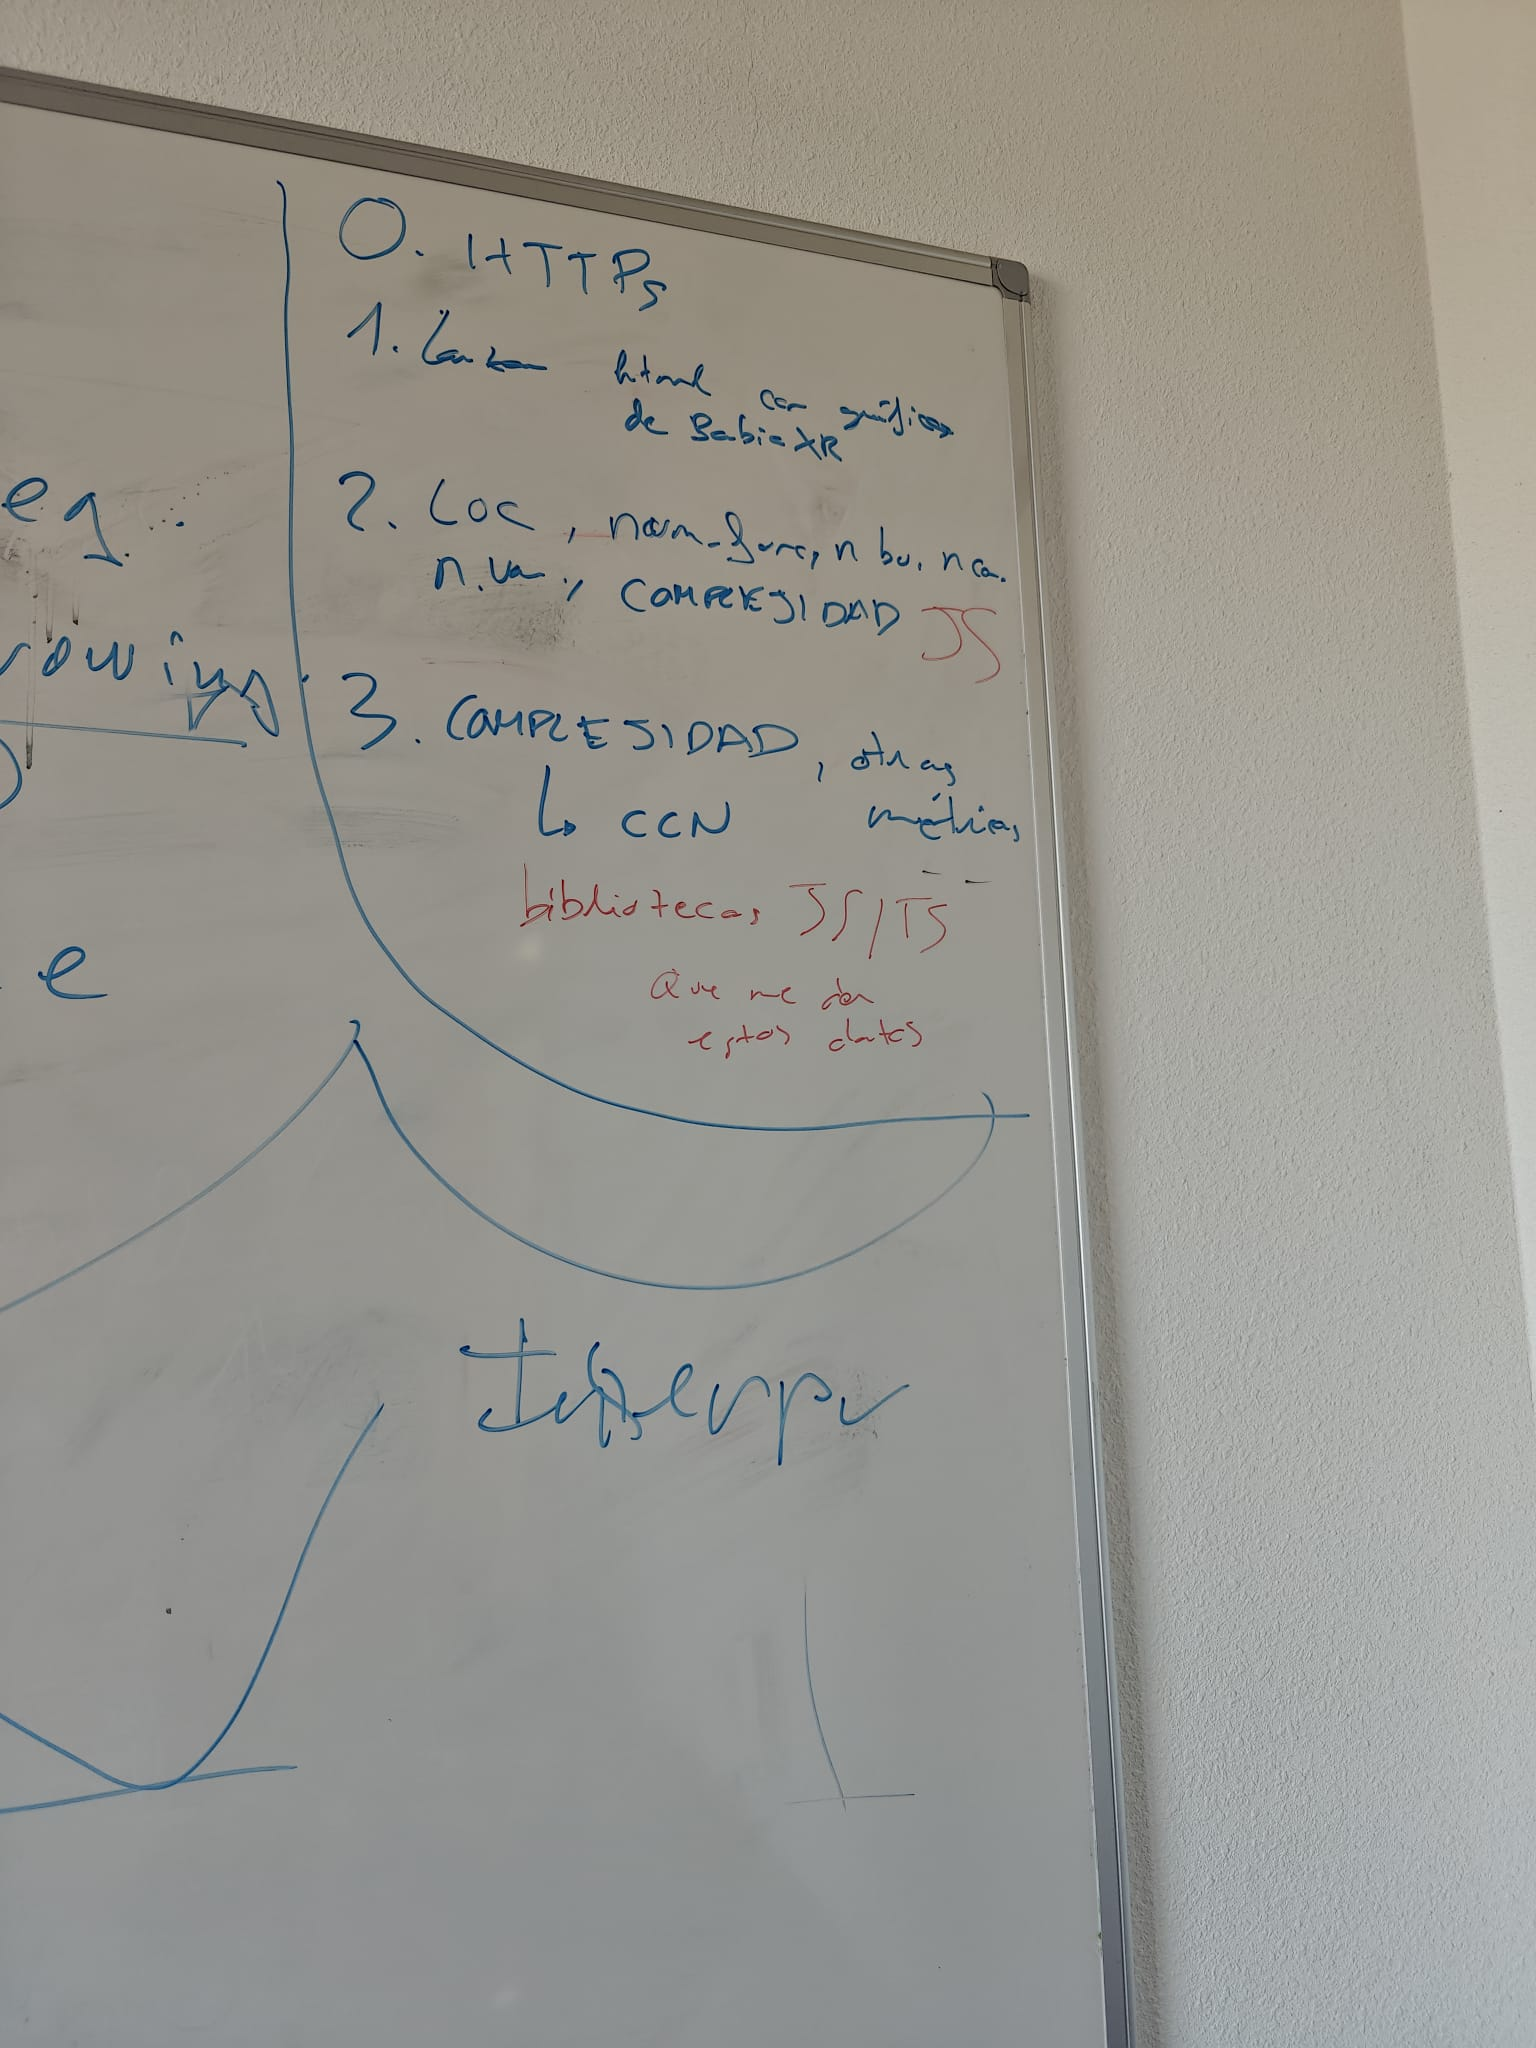
\includegraphics[width=0.4\textwidth]{img/reunion_2025-03-12.png}
    \caption{Imagen de la reunión del 12 de marzo de 2025, donde se definieron los puntos principales del TFG.}
    \label{fig:reunion-marzo}
\end{figure}


\begin{figure}[H]
\centering
\begin{adjustbox}{width=\textwidth,center}
\begin{ganttchart}[
    x unit=0.7cm,
    y unit title=0.8cm,
    y unit chart=0.7cm,
    vgrid,
    hgrid,
    title/.append style={draw=none, fill=blue!20},
    title height=1,
    bar/.append style={draw=black, fill=blue!40},
    bar height=0.6,
    group/.append style={draw=black, fill=green!30},
    milestone/.append style={draw=red, fill=red, shape=diamond},
    milestone height=0.6
]{1}{24}

% Títulos de los meses
\gantttitle{Planificación temporal de Code-XR}{24} \\
\gantttitle{Enero}{4} 
\gantttitle{Febrero}{4} 
\gantttitle{Marzo}{4} 
\gantttitle{Abril}{4} 
\gantttitle{Mayo}{4} 
\gantttitle{Junio}{2} 
\gantttitle{Julio}{2} \\

% Tareas principales
\ganttgroup{Fase inicial y contacto}{1}{8} \\
\ganttbar{Propuesta de TFG por tutor}{1}{1} \\
\ganttbar{Evaluación de temáticas}{5}{8} \\

\ganttgroup{Definición del proyecto}{9}{12} \\
\ganttbar{Decisión final: Plugin VS Code}{9}{9} \\
\ganttbar{Exploración extensiones VS Code}{10}{11} \\
\ganttmilestone{Reunión presencial}{12} \\

\ganttgroup{Desarrollo núcleo}{13}{16} \\
\ganttbar{Análisis de código (Lizard)}{13}{14} \\
\ganttbar{Modo LivePanel}{13}{14} \\
\ganttbar{Análisis en tiempo real (SSE)}{14}{16} \\
\ganttmilestone{Publicación Code-XR}{14} \\

\ganttgroup{Pausa por exámenes}{17}{20} \\
\ganttbar{Sin desarrollo activo}{17}{20} \\

\ganttgroup{Funcionalidades avanzadas}{21}{22} \\
\ganttbar{VisualizeDOM}{21}{21} \\

\ganttgroup{Finalización y publicación}{23}{24} \\
\ganttbar{Análisis de directorios}{23}{24} \\
\ganttbar{Configuraciones avanzadas}{23}{24} \\
\ganttbar{Perfiles personalizados}{23}{24} \\
\ganttmilestone{Versión 1.0.0 y web oficial}{24} \\

% Enlaces entre tareas
\ganttlink{elem1}{elem2}
\ganttlink{elem4}{elem5}
\ganttlink{elem6}{elem7}
\ganttlink{elem9}{elem12}

\end{ganttchart}
\end{adjustbox}
\caption{Diagrama de Gantt de la planificación temporal de Code-XR (enero-julio 2025).}
\label{fig:gantt-codexr}
\end{figure}


%%%%%%%%%%%%%%%%%%%%%%%%%%%%%%%%%%%%%%%%%%%%%%%%%%%%%%%%%%%%%%%%%%%%%%%%%%%%%%%%
%%%%%%%%%%%%%%%%%%%%%%%%%%%%%%%%%%%%%%%%%%%%%%%%%%%%%%%%%%%%%%%%%%%%%%%%%%%%%%%%
% ESTADO DEL ARTE %
%%%%%%%%%%%%%%%%%%%%%%%%%%%%%%%%%%%%%%%%%%%%%%%%%%%%%%%%%%%%%%%%%%%%%%%%%%%%%%%%

\cleardoublepage
\chapter{Estado del arte}
\label{chap:estado}

\section{Visual Studio Code y su sistema de extensiones}
\label{sec:vscode}

Visual Studio Code (VS Code) es un editor de código fuente desarrollado por Microsoft, ampliamente adoptado por su ligereza, extensibilidad y soporte para múltiples lenguajes. Su éxito se debe tanto a funcionalidades integradas (autocompletado, depuración, integración con Git) como a su ecosistema de extensiones.

El sistema de extensiones permite ampliar el editor mediante plugins basados en tecnologías web (TypeScript, JavaScript, HTML y CSS), que interactúan con el entorno a través de la API oficial de VS Code~\cite{vscode-api}. Esta API ofrece acceso al árbol de archivos, edición de documentos, creación de paneles personalizados, ejecución de comandos y gestión de eventos internos.

En este TFG, VS Code se ha empleado tanto como entorno de desarrollo como plataforma de despliegue de Code-XR. Su elección responde a dos motivos: técnico, al posibilitar la integración de visualizaciones de métricas directamente en el flujo de trabajo del programador sin cambios de contexto; y personal, por ser el editor utilizado a lo largo de mi formación académica.  

Gracias a la API de extensiones~\cite{vscode-api}, ha sido posible registrar comandos, interceptar eventos y lanzar servidores locales que conectan el análisis estático con las visualizaciones XR. El modelo modular y orientado a eventos de VS Code lo convierte en un entorno idóneo para herramientas como Code-XR, que requieren sincronización en tiempo real con el proceso de edición.

\section{BabiaXR}
\label{sec:babiaxr}

BabiaXR~\cite{moreno2022babiaxr} es una plataforma de visualización tridimensional e inmersiva desarrollada por investigadores del Grupo de Sistemas y Comunicaciones (GSyC) de la Universidad Rey Juan Carlos (URJC). Está diseñada para facilitar la creación de escenas interactivas en realidad extendida (XR), incluyendo realidad virtual (VR)y aumentada (AR), utilizando tecnologías web abiertas y accesibles como A-Frame, Three.js y WebXR.

El objetivo de BabiaXR es proporcionar un entorno modular y fácilmente integrable que permita a desarrolladores e investigadores visualizar información compleja de forma espacial, sin necesidad de conocimientos avanzados de gráficos 3D. Gracias a su arquitectura basada en componentes personalizables, BabiaXR permite representar datos estructurados como visualizaciones 3D interactivas, directamente desde el navegador y sin necesidad de instalar software adicional. Esto lo convierte en una herramienta especialmente útil en contextos educativos y científicos, donde la simplicidad de despliegue y la portabilidad son factores clave.

En el contexto de este TFG, BabiaXR se ha utilizado como motor base para renderizar las visualizaciones XR de métricas de software generadas por el plugin Code-XR. Concretamente, se han empleado varios de sus componentes gráficos para representar las distintas métricas sobre ficheros o directorios.

% PONER MAS ADELANTE LA FIGURA DE LOS GRAFICOS DE BABIAXR
% \begin{figure}[H]
%     \centering
%     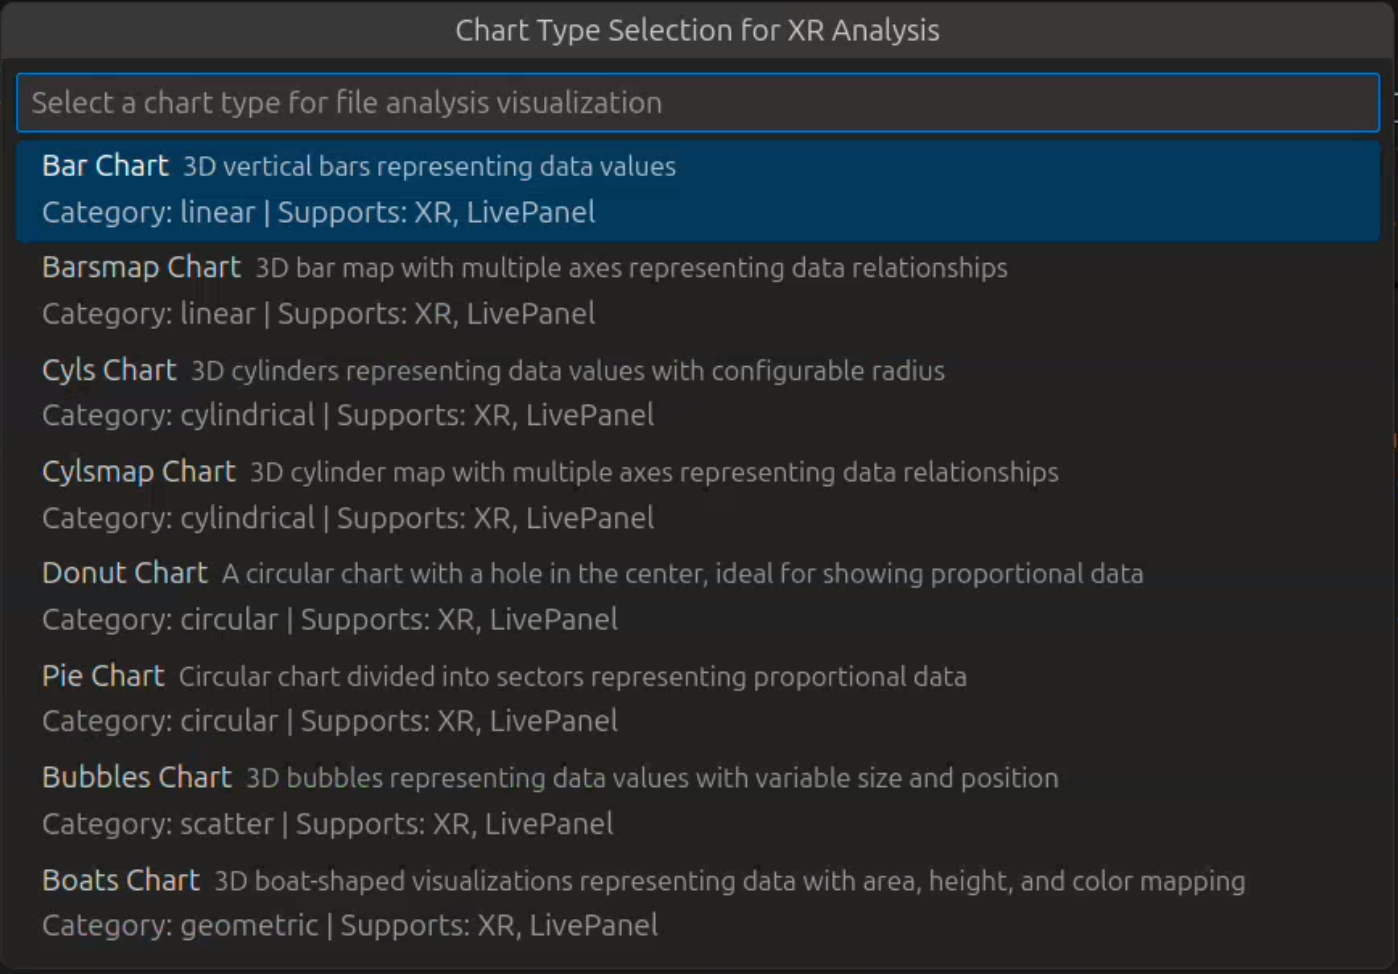
\includegraphics[width=0.85\textwidth]{img/graficos_babiaxr.png}
%     \caption{Ejemplo de los diferentes gráficos de BabiaXR utilizados en Code-XR para la visualización de métricas.}
%     \label{fig:babiaxr-graficos}
% \end{figure}

\section{A-Frame}
\label{sec:aframe}

A-Frame es un framework de código abierto desarrollado por Mozilla para crear experiencias inmersivas de realidad virtual y aumentada desde el navegador~\cite{aframe}. Ofrece una sintaxis declarativa en HTML que simplifica la definición de escenas 3D, actuando como capa de abstracción sobre Three.js y permitiendo el uso de componentes modulares y extensibles.  

En Code-XR, A-Frame constituye el motor principal de visualización XR: cada análisis inmersivo se representa en una escena \texttt{<a-scene>} que integra el entorno, los datos analizados, gráficos tridimensionales (bar, city, etc.) y controladores de interacción tanto para escritorio como para dispositivos XR. Extensiones como \texttt{aframe-extras}, \texttt{aframe-environment-component} y \texttt{aframe-geometry-merger-component} mejoran la navegación, los entornos predefinidos y el rendimiento en escenas complejas.  

Gracias a esta infraestructura, Code-XR permite explorar métricas de código en entornos tridimensionales interactivos sin necesidad de conocimientos avanzados en gráficos 3D, ofreciendo una experiencia inmersiva directamente integrada en el flujo de trabajo del desarrollador.

\section{WebXR y Three.js}
\label{sec:webxr-threejs}

WebXR es el estándar del W3C que unifica el acceso a dispositivos de realidad virtual y aumentada desde navegadores modernos~\cite{webxr}. Sustituye a WebVR al soportar VR y AR desde una misma API, permitiendo experiencias multiplataforma que responden en tiempo real a la posición y orientación del usuario. Aunque Code-XR no usa WebXR de forma explícita, sus capacidades están presentes a través de BabiaXR y A-Frame, lo que posibilita ejecutar visualizaciones XR inmersivas directamente en el navegador o en dispositivos como Meta Quest sin configuraciones adicionales.  

Por su parte, Three.js es la biblioteca de JavaScript que facilita el renderizado 3D en WebGL~\cite{threejs}, proporcionando primitivas para cámaras, luces, materiales o geometrías. A-Frame se apoya en ella como motor de bajo nivel, de modo que aunque no se use directamente en Code-XR, resulta esencial para representar métricas en forma de ciudades 3D, jerarquías DOM navegables o escenas con decenas de elementos manteniendo fluidez y compatibilidad en distintos navegadores.  

En conjunto, WebXR y Three.js, aun sin estar programadas directamente en este TFG, constituyen la base tecnológica que hace posible la inmersión y el rendimiento gráfico de Code-XR a través de los frameworks que las encapsulan.


\section{HTML}
\label{sec:html}

HTML (HyperText Markup Language) es el lenguaje de marcado esencial para estructurar contenido web~\cite{html} y constituye la base de todas las interfaces de Code-XR, ya sea en LivePanel, XR Mode o VisualizeDOM.  

Cada vez que se lanza un análisis, el sistema genera dinámicamente una plantilla HTML que incluye scripts, referencias a datos y configuraciones específicas según el modo. Estas plantillas se sirven desde un servidor local, accesibles tanto en navegador como en un panel de VS Code.  

En LivePanel, HTML organiza métricas en tablas o tarjetas interactivas; en XR Mode define escenas 3D con A-Frame mediante elementos como \texttt{<a-scene>} y \texttt{<a-entity>}; y en VisualizeDOM representa la estructura del DOM como un árbol navegable.  

El uso de HTML aporta versatilidad y compatibilidad con el ecosistema web, lo que facilita la incorporación de bibliotecas, componentes personalizados e interacciones, manteniendo una arquitectura visual coherente y extensible en todos los modos de la herramienta.

\section{TypeScript y JavaScript}
\label{sec:typescript-javascript}

TypeScript, desarrollado por Microsoft, extiende JavaScript con tipado estático y características orientadas a objetos~\cite{typescript}. En Code-XR constituye el motor principal del plugin, encargado de la lógica de control, la integración con la API de VS Code, la gestión de análisis de ficheros y directorios, el lanzamiento de servidores locales y la orquestación de las visualizaciones (LivePanel, XR Mode, VisualizeDOM). Su sistema de tipos aporta robustez y mantenibilidad al proyecto.

JavaScript, por su parte, se utiliza en el cliente para la actualización dinámica de las visualizaciones~\cite{javascript}. Implementa la comunicación en tiempo real mediante Server-Sent Events (SSE), de modo que cada cambio en el código provoca la actualización inmediata de los datos en la interfaz. En el caso del LivePanel, se encarga de inyectar y actualizar dinámicamente el HTML con métricas en tablas, tarjetas o gráficos.

La combinación de TypeScript para la lógica central y de JavaScript para la capa de presentación ha permitido construir una herramienta modular, interactiva y eficiente, alineada con las prácticas modernas de desarrollo web.

\section{CSS}
\label{sec:css}

CSS (Cascading Style Sheets) es el lenguaje estándar para definir la presentación visual de documentos HTML~\cite{css}. En Code-XR se emplea para dar estilo a las plantillas HTML generadas en el modo LivePanel, donde se muestran métricas como líneas de código, complejidad ciclomática o número de parámetros. Su uso permite resaltar valores según la complejidad, organizar la información en tarjetas y adaptar la visualización a distintos tamaños de ventana. Aunque no interviene en los modos XR inmersivos ni en la representación tridimensional del DOM, CSS cumple un papel clave en la experiencia de usuario de las visualizaciones 2D, manteniendo una arquitectura modular al separar el estilo de la lógica de análisis y comunicación.

\section{Python y Lizard}
\label{sec:python-lizard}

Python es un lenguaje de alto nivel ampliamente utilizado en automatización y análisis de datos~\cite{python}, y en Code-XR se emplea para realizar el análisis estático del código fuente. Desde el backend del plugin, escrito en TypeScript, se lanzan scripts en Python que procesan ficheros o directorios y generan un fichero JSON con las métricas calculadas.  

Para obtener métricas como complejidad ciclomática (CCN), líneas de código (LOC) o número de funciones, se utiliza Lizard~\cite{lizard}, una biblioteca de análisis estático compatible con múltiples lenguajes que devuelve una representación estructurada de los componentes del código. Estos datos alimentan tanto al modo LivePanel (visualización 2D) como al modo XR (ciudad 3D), donde se mapean propiedades como tamaño o complejidad a atributos visuales como altura, color o volumen.  

Además, en el modo VisualizeDOM, Python se encarga de leer archivos HTML y transformarlos en una cadena que el componente \texttt{babia-html} interpreta para generar la visualización tridimensional. En conjunto, la integración de Python y Lizard proporciona datos estáticos fiables y estructurados, fundamentales para las visualizaciones de Code-XR en todos sus modos.

\section{Gafas de Realidad Virtual: Meta Quest 3}
\label{sec:meta-quest-3}

Para validar las funcionalidades inmersivas de Code-XR se utilizaron gafas de realidad virtual Meta Quest 3~\cite{metaquest3}, cedidas temporalmente por la Universidad Rey Juan Carlos. Estos dispositivos, capaces de ejecutar experiencias VR de forma autónoma gracias a su procesador y sensores integrados, se conectaron al servidor local del plugin para acceder a las visualizaciones XR.  

Su uso permitió comprobar en condiciones reales el funcionamiento del modo XR, ajustar la navegación y la disposición de los gráficos, y evaluar el rendimiento general. Además, fueron fundamentales para verificar la integración con WebXR y la representación de métricas complejas en escenarios tridimensionales navegables.


\section{Apoyo de herramientas de inteligencia artificial}
\label{sec:ia}

Durante el desarrollo se emplearon herramientas de inteligencia artificial como apoyo para resolver dudas técnicas, explorar alternativas y aprender nuevas tecnologías.  

ChatGPT~\cite{chatgpt} fue clave para comprender bibliotecas como Lizard (análisis estático de código) o A-Frame (escenas XR), así como para proponer soluciones a problemas concretos, mejorar la organización del código y redactar documentación técnica más clara.  

Claude 4~\cite{claude4} se utilizó principalmente en la gestión y organización de grandes volúmenes de código, especialmente útil en un repositorio con más de 200 ficheros en la carpeta \texttt{src/}.  

Estas herramientas no sustituyen el conocimiento propio, pero sí aportaron valor al desarrollo al mejorar la eficiencia y la claridad en distintas partes del proyecto.


%%%%%%%%%%%%%%%%%%%%%%%%%%%%%%%%%%%%%%%%%%%%%%%%%%%%%%%%%%%%%%%%%%%%%%%%%%%%%%%%
%%%%%%%%%%%%%%%%%%%%%%%%%%%%%%%%%%%%%%%%%%%%%%%%%%%%%%%%%%%%%%%%%%%%%%%%%%%%%%%%
% DISEÑO E IMPLEMENTACIÓN %
%%%%%%%%%%%%%%%%%%%%%%%%%%%%%%%%%%%%%%%%%%%%%%%%%%%%%%%%%%%%%%%%%%%%%%%%%%%%%%%%

\cleardoublepage
\chapter{Diseño e implementación}
\label{sec:diseno}

% Aquí viene todo lo que has hecho tú (tecnológicamente). 
% Puedes entrar hasta el detalle. 
% Es la parte más importante de la memoria, porque describe lo que has hecho tú.
% Eso sí, normalmente aconsejo no poner código, sino diagramas.



% \section{Arquitectura general} 
% \label{sec:arquitectura}

% Si tu proyecto es un software, siempre es bueno poner la arquitectura (que es cómo se estructura tu programa a ``vista de pájaro'').

% \begin{figure}
%   \centering
%   \includegraphics[width=9cm, keepaspectratio]{img/arquitectura.png}
%   \caption{Estructura del parser básico}
%   \label{fig:arquitectura}
% \end{figure}


% Por ejemplo, puedes verlo en la figura~\ref{fig:arquitectura}.
% \LaTeX \ pone las figuras donde mejor cuadran. 
% Y eso quiere decir que quizás no lo haga donde lo hemos puesto\ldots 
% Eso no es malo.
% A veces queda un poco raro, pero es la filosofía de \LaTeX: tú al contenido, que yo me encargo de la maquetación.


 
% Recuerda que toda figura que añadas a tu memoria debe ser explicada.
% Sí, aunque te parezca evidente lo que se ve en la figura~\ref{fig:arquitectura}, la figura en sí solamente es un apoyo a tu texto.
% Así que explica lo que se ve en la figura, haciendo referencia a la misma tal y como ves aquí.
% Por ejemplo: En la figura~\ref{fig:arquitectura} se puede ver que la estructura del \emph{parser} básico, que consta de seis componentes diferentes: los datos se obtienen de la red, y según el tipo de dato, se pasará a un \emph{parser} específico y bla, bla, bla\ldots

% Si utilizas una base de datos, no te olvides de incluir también un diagrama de entidad-relación.


% \section{Arquitectura general} 
% \label{sec:arquitectura}

% En esta sección se presenta la arquitectura general de Code‑XR, explicando sus componentes principales, los canales de comunicación entre ellos y las decisiones tecnológicas que sustentan su diseño. El objetivo es ofrecer una visión global suficiente para entender cómo fluye la información desde el código fuente hasta las visualizaciones en 2D (LivePanel) y XR.

% En los siguientes apartados de este capítulo se explicará cómo se desarrollaron las distintas partes del plugin, los pasos o sprints seguidos durante el desarrollo y cómo se estableció la comunicación entre los componentes, incluyendo detalles sobre protocolos, formatos de intercambio y la orquestación entre TypeScript, Python y las vistas cliente.


% \subsection{Componentes y responsabilidades}
% \begin{itemize}
%   \item \textbf{VS Code Extension (TypeScript):} registro de comandos, UI en el editor, gestión de procesos (lanzamiento de servidores HTTP/HTTPS, análisis con Python mediante entorno virtual, etc...), y almacenamiento de configuraciones. En conclusión, TypeScript es el lenguaje que maneja toda la lógica del plugin a través de la API oficial de Visual Studio Code~\cite{vscode-api}.
%   \item \textbf{Python metrics engine:} ejecución de scripts en Python para el análisis estático de ficheros y directorios. La mayor parte de las métricas se extraen usando la librería Lizard~\cite{lizard}, mientras que algunas métricas complementarias se calculan mediante código Python propio. El resultado se normaliza y se exporta en formato JSON para ser entendido por los componentes de BabiaXR~\cite{moreno2022babiaxr}.
%   \item \textbf{JSON Storage / Manager:} formato intermedio y almacenamiento temporal de resultados (ficheros .json o memoria). Este formato se utiliza tanto para las configuraciones del plugin —por ejemplo, parámetros a representar y el tipo de gráfico seleccionado— como para la salida de los análisis ejecutados por Python (las métricas se exportan en JSON). Las configuraciones persistentes del plugin se guardan usando la API de VS Code en globalState (ExtensionContext.globalState), de modo que se mantienen entre sesiones del editor; por su parte, los resultados de análisis y datos asociados al proyecto se almacenan en workspaceState (ExtensionContext.workspaceState), que queda ligado al workspace abierto y no se comparte entre workspaces. Para más detalles sobre ambos mecanismos de almacenamiento véase la documentación oficial de VS Code~\cite{vscode-storage}.
%   \item \textbf{Realtime API (SSE):} canal unidireccional basado en Server‑Sent Events (SSE) para enviar actualizaciones incrementales de métricas a los clientes (LivePanel, XR). En el cliente se implementa mediante la API nativa `EventSource` de JavaScript, y en el servidor mediante respuestas HTTP con content‑type \texttt{text/event-stream}~\cite{mdn-sse}. 

%   Aunque existen librerías como express-sse~\cite{express-sse} que facilitan la implementación de SSE en aplicaciones Node.js, se optó por una implementación nativa para mantener un control granular sobre los eventos enviados y reducir las dependencias externas del plugin. El sistema funciona de la siguiente manera: cuando un fichero observado cambia, la extensión detecta la modificación, lanza un re‑análisis (entorno virtual de Python), normaliza y actualiza el JSON correspondiente en workspaceState, y emite eventos SSE específicos como \texttt{analysis-updated} o \texttt{dataRefresh}. Los clientes suscritos (LivePanel, páginas XR) escuchan estos eventos mediante \texttt{EventSource('/events')}, reciben las notificaciones y actualizan automáticamente las visualizaciones sin recargar la página.
%   \item \textbf{Servidores de visualización (HTML/CSS/JS):} conjunto de plantillas web servidas por servidores locales HTTP/HTTPS para la visualización de métricas. Incluye dos modos principales:
%   \begin{itemize}
%     \item \textbf{LivePanel}: webview embebida en VS Code para visualización 2D con tablas, gráficos y métricas detalladas.
%     \item \textbf{XR Pages}: escenas 3D basadas en A-Frame y BabiaXR para visualización inmersiva en navegador o dispositivos VR.
%   \end{itemize}
%   Ambos modos comparten la misma infraestructura de servidor y comunicación SSE. Para el acceso desde dispositivos XR (como Meta Quest 3), el servidor debe configurarse en modo HTTPS con certificados autofirmados generados mediante OpenSSL~\cite{openssl}, ya que los navegadores en dispositivos VR requieren conexiones seguras para acceder a las APIs de WebXR.
%   \item \textbf{Sistema de plantillas dinámicas:} generador automático de plantillas HTML específicas para cada tipo de análisis y visualización. Incluye procesamiento de placeholders, validación de dimensiones de datos, y adaptadores para diferentes gráficos BabiaXR según el tipo de métricas extraídas.
%   \item \textbf{File watcher y detección de cambios:} monitorización automática de archivos para re-análisis en tiempo real. Utiliza la API de VS Code para detectar modificaciones en los ficheros bajo análisis y triggear actualizaciones automáticas del JSON y las vistas asociadas.
%   \item \textbf{Registry de servidores activos:} sistema de registro y gestión del ciclo de vida de servidores HTTP/HTTPS lanzados por el plugin. Permite controlar múltiples instancias simultáneas, gestionar puertos dinámicos y evitar conflictos entre diferentes análisis en ejecución.
% \end{itemize}


% % ...existing code...
% \subsection{Tipos de análisis}
% \label{sec:tipos-analisis}

% A continuación se presenta una tabla simplificada con los tipos fundamentales de análisis soportados por Code‑XR, su alcance y si admiten la opción \emph{deep} (recursión por subdirectorios) o la posibilidad de aplicarse al workspace completo (análisis de proyecto).

% \begin{figure}[H]
% \centering\small
% \begin{tabular}{p{5.0cm} p{7.5cm} p{2.5cm}}
% \hline
% \textbf{Tipo de análisis} & \textbf{Alcance} & \textbf{Deep? / Proyecto?} \\
% \hline
% Fichero — LivePanel & Análisis puntual de un único fichero; visualización 2D en el panel integrado. & No / No \\
% Fichero — XR & Análisis puntual de un único fichero; representación inmersiva en A‑Frame/BabiaXR. & No / No \\
% Directorio — LivePanel & Análisis de un directorio; resumen por archivo y agregados por carpeta. & Sí / Sí \\
% Directorio — XR & Representación 3D del contenido de un directorio (escena A‑Frame/BabiaXR). & Sí / Sí \\
% DOM Mode (especial) & Análisis de la estructura DOM de un fichero HTML; visualización 3D específica del DOM. & No / No \\
% \hline
% \end{tabular}
% \caption{Tipos fundamentales de análisis, alcance y soporte de \emph{deep}/\emph{proyecto}.}
% \label{tab:tipos-analisis}
% \end{figure}

% \bigskip

% \noindent Para mayor claridad, a continuación se muestra la relación entre los comandos expuestos en la interfaz (menú contextual / editor) y el tipo de análisis que lanzan.


% \begin{figure}[H]
% \centering\small
% \begin{tabular}{p{9.0cm} p{6.0cm}}
% \hline
% \textbf{Comando (UI)} & \textbf{Identificador interno / Tipo} \\
% \hline
% CodeXR: Analyze File (LivePanel) & \texttt{newCodeAnalysis.analyzeFile} — Fichero / LivePanel \\
% CodeXR: Analyze File (XR) & \texttt{newCodeAnalysis.analyzeFileXR} — Fichero / XR \\
% CodeXR: Analyze Directory (LivePanel) & \texttt{newCodeAnalysis.analyzeDirectory} — Directorio / LivePanel (No deep) \\
% CodeXR: Analyze Directory (LivePanel Deep) & \texttt{newCodeAnalysis.analyzeDirectoryDeep} — Directorio / LivePanel (Deep) \\
% CodeXR: Analyze Directory (XR) & \texttt{newCodeAnalysis.analyzeDirectoryXR} — Directorio / XR (No deep) \\
% CodeXR: Analyze Directory (XR Deep) & \texttt{newCodeAnalysis.analyzeDirectoryXRDeep} — Directorio / XR (Deep) \\
% CodeXR: Analyze Project (LivePanel) & \texttt{newCodeAnalysis.analyzeProject} — Proyecto / LivePanel (raíz del workspace) \\
% CodeXR: Analyze Project (LivePanel Deep) & \texttt{newCodeAnalysis.analyzeProjectDeep} — Proyecto / LivePanel (Deep, raíz del workspace) \\
% CodeXR: Analyze Project (XR) & \texttt{newCodeAnalysis.analyzeProjectXR} — Proyecto / XR (raíz del workspace) \\
% CodeXR: Analyze Project (XR Deep) & \texttt{newCodeAnalysis.analyzeProjectXRDeep} — Proyecto / XR (Deep, raíz del workspace) \\
% CodeXR: Visualize DOM & \texttt{newCodeAnalysis.visualizeDOM} — DOM Mode \\
% \hline
% \end{tabular}
% \caption{Mapeo entre comandos de la UI y tipos de análisis (incluye variantes de proyecto).}
% \label{tab:comandos-analisis}
% \end{figure}

% \bigskip


% Notas:
% \begin{itemize}
%   \item Los comandos de ``Proyecto'' operan reutilizando la misma lógica interna que los comandos de ``Directorio''; la única diferencia es que, al invocarse, toman la raíz del workspace como directorio a analizar.
%   \item La forma de invocar estos comandos desde la interfaz es mediante el menú contextual (click derecho) en el explorador de archivos o en el editor. La asignación de entradas de menú, reglas de visibilidad y los identificadores de comando están declarados en el fichero \texttt{package.json} del plugin; en un apartado posterior se detalla la estructura y funcionamiento de \texttt{package.json} en extensiones de VS Code. Otra forma también de invocarlos es a través de un acceso rápido integrado en la interfaz del plugin, que permite seleccionar ficheros y directorios mediante las vistas ``Files by Language'' y ``Project Structure''. Esto se explicará con más detalle en la sección dedicada a la interfaz del plugin.
%   \item ``Deep'' indica análisis recursivo sobre subdirectorios; su uso incrementa la cantidad de datos y las entidades en la escena XR, por lo que puede requerir optimizaciones de rendimiento (batching, análisis incremental, reducción de nivel de detalle).
% \end{itemize}


% Explicacion de la evolucion del proyecto


%--------------------------------
% Resumen cronológico de versiones
%--------------------------------
\section{Resumen cronológico de versiones}
\label{sec:resumen-versiones}
A continuación se presenta un resumen cronológico de las versiones principales del plugin (0.0.1 → 1.0.0), condensando los hitos de desarrollo más relevantes.

\begin{table}[!htbp]
\centering\footnotesize
\begin{tabular}{p{1.8cm} p{2.2cm} p{10.5cm}}
\hline
\textbf{Versión} & \textbf{Fecha} & \textbf{Hito principal} \\
\hline
0.0.1 & 2025-03-11 & Prototipo inicial: servidor HTTP con escena A‑Frame básica y comandos de lanzamiento. \\
0.0.2 & 2025-03-20 & Análisis básico LivePanel (JS/TS), infraestructura XR inicial, verificaciones HTTPS. \\
0.0.3 & 2025-04-11 & Auto‑reanalysis, SSE, watchers, análisis estático (LOC, CCN, funciones). \\
0.0.4 & 2025-04-27 & Soporte multi‑lenguaje, debounce configurable, análisis múltiple simultáneo. \\
0.0.5 & 2025-04-29 & Visualizaciones babia‑boats, mapeo parámetros‑dimensiones visuales. \\
0.0.6 & 2025-04-29 & Publicación inicial marketplace, estabilización servidores y UX. \\
0.0.7 & 2025-06-01 & Live reload mejorado, controles VR/AR, configuración avanzada entornos. \\
0.0.8 & 2025-07-03 & Motor análisis revisado: Lizard ampliado, VisualizeDOM, bubble charts. \\
0.0.9 & 2025-07-27 & Re‑arquitecturación: análisis directorios completos, soporte deep, optimizaciones. \\
1.0.0 & 2025-07-28 & Versión estable: auto‑análisis configurable, gestión sesiones, web oficial. \\
\hline
\end{tabular}
\caption{Resumen cronológico de versiones principales del desarrollo de Code-XR.}
\label{tab:changelog}
\end{table}


\noindent \textbf{Nota:} Detalles extraídos del fichero \texttt{CHANGELOG.md}. Registros públicos desde v0.0.3, marketplace desde v0.0.6.


% Diagrama temporal simplificado de la evolución de versiones
\begin{figure}[H]
  \centering
  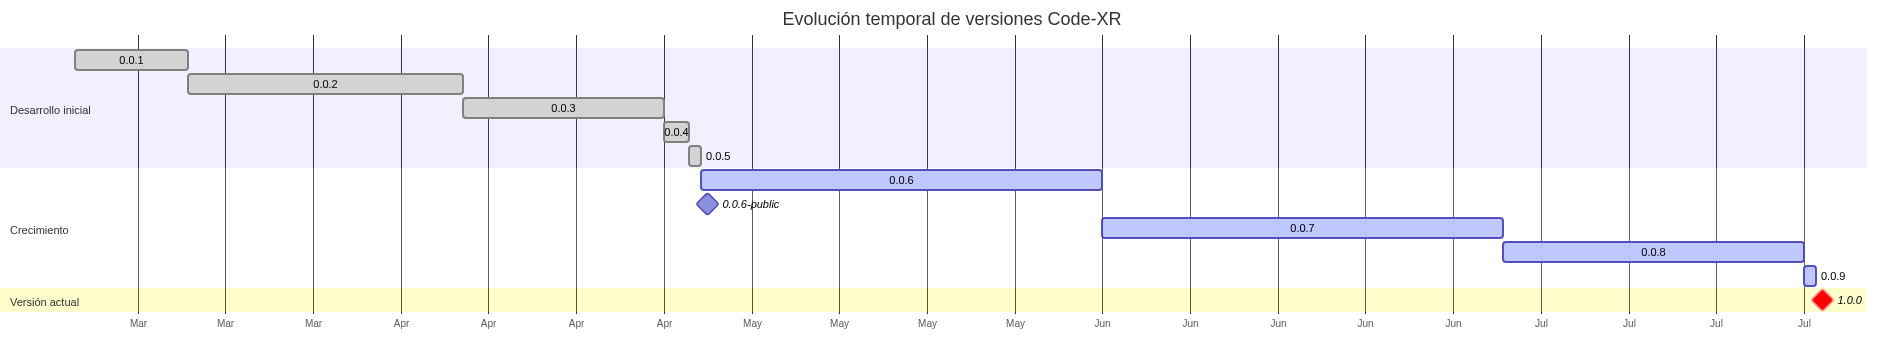
\includegraphics[width=\textwidth]{img/versions_gantt.png}
  \caption{Evolución temporal resumida de las versiones principales del proyecto.}
  \label{fig:timeline-versions}
\end{figure}
% ...existing


\noindent En los siguientes subapartados se describirán los sprints/hitos que explican cómo se pasó de la idea inicial a la versión 1.0.0, detallando para cada sprint el objetivo, las tareas realizadas y los artefactos resultantes.

%--------------------------------
% Primeros pasos
%--------------------------------

\section{Primeros pasos}
\label{sec:primeros-pasos}

Esta sección presenta las decisiones técnicas iniciales para crear la extensión de VS Code. Se siguió el tutorial oficial\cite{tutorialVSCode} y recursos complementarios\cite{vscode-youtube}, utilizando el generador ``Yo Code''\cite{yo-code} para establecer las bases del proyecto.

\subsection{Generador \emph{Yo Code}}
El generador oficial ``Yo Code'' configura la plantilla inicial mediante preguntas sobre identificador, descripción, lenguaje de desarrollo (TypeScript/JavaScript), repositorio Git y tipo de empaquetado (\emph{unbundled}, Webpack, Esbuild). Estas decisiones configuran la estructura base y scripts de compilación.

\subsection{Elección de lenguaje}
Se eligió \textbf{TypeScript} por su tipado estático, integración directa con la API de VS Code y mejor mantenibilidad en proyectos complejos\cite{typescript}. Permitió la evolución segura de Code-XR al crecer en ficheros y complejidad.

\subsection{Bundlers}
El empaquetado puede realizarse de distintas formas según las necesidades del proyecto\cite{vscode-bundling}:
\begin{itemize}
  \item \textbf{Unbundled}: sin bundler, prototipado rápido pero distribución manual de dependencias.
  \item \textbf{Webpack}: bundler establecido, genera paquete único y minimiza dependencias\cite{webpack}.
  \item \textbf{Esbuild}: bundler moderno con compilación extremadamente rápida\cite{esbuild}.
\end{itemize}

Code-XR comenzó con \emph{unbundled} para prototipado rápido, migrando posteriormente a \textbf{Webpack} para mayor fiabilidad y resolver advertencias de \texttt{npm} por tamaño excesivo en el empaquetado \texttt{.vsix}.

\subsection{Archivo \texttt{package.json} (manifiesto de la extensión)}
El \texttt{package.json} es el manifiesto central con metadatos del Marketplace, compatibilidad con VS Code y configuración de compilación. La sección \texttt{contributes} define los elementos de interfaz: +40 comandos, vista \texttt{codexrTree} y menús contextuales\cite{vscode-bundling}.

Code-XR utiliza activación ansiosa (lista vacía en \texttt{activationEvents}) para garantizar disponibilidad inmediata de menús y vistas. La iconografía combina \emph{Codicons}\cite{codicons} oficiales, iconos \emph{Devicon}\cite{devicon} para representación de ficheros, y logotipo personalizado generado con IA.

\subsection{Archivo \texttt{extension.ts}}
Implementa la lógica del manifiesto como punto de entrada con dos funciones principales:
\begin{itemize}
  \item \texttt{activate}: inicializa servicios, registra vistas y comandos, sincroniza estado.
  \item \texttt{deactivate}: libera recursos (servidores, gestores SSE, mapeos).
\end{itemize}

Garantiza arranque limpio y cierre ordenado sin procesos residuales.

\subsection{Registro de comandos e interfaz de usuario}
Los comandos conectan acciones de usuario con lógica interna: declaración en \texttt{package.json} y enlace en \texttt{extension.ts}. La interfaz utiliza primitivas de VS Code:
\begin{itemize}
  \item \textbf{TreeView / TreeDataProvider}: organización en vista lateral.
  \item \textbf{WebviewPanel / WebviewView}: visualizaciones 2D/XR interactivas.
  \item \textbf{StatusBarItem}: notificaciones y accesos directos.
\end{itemize}

\begin{figure}[H]
\centering
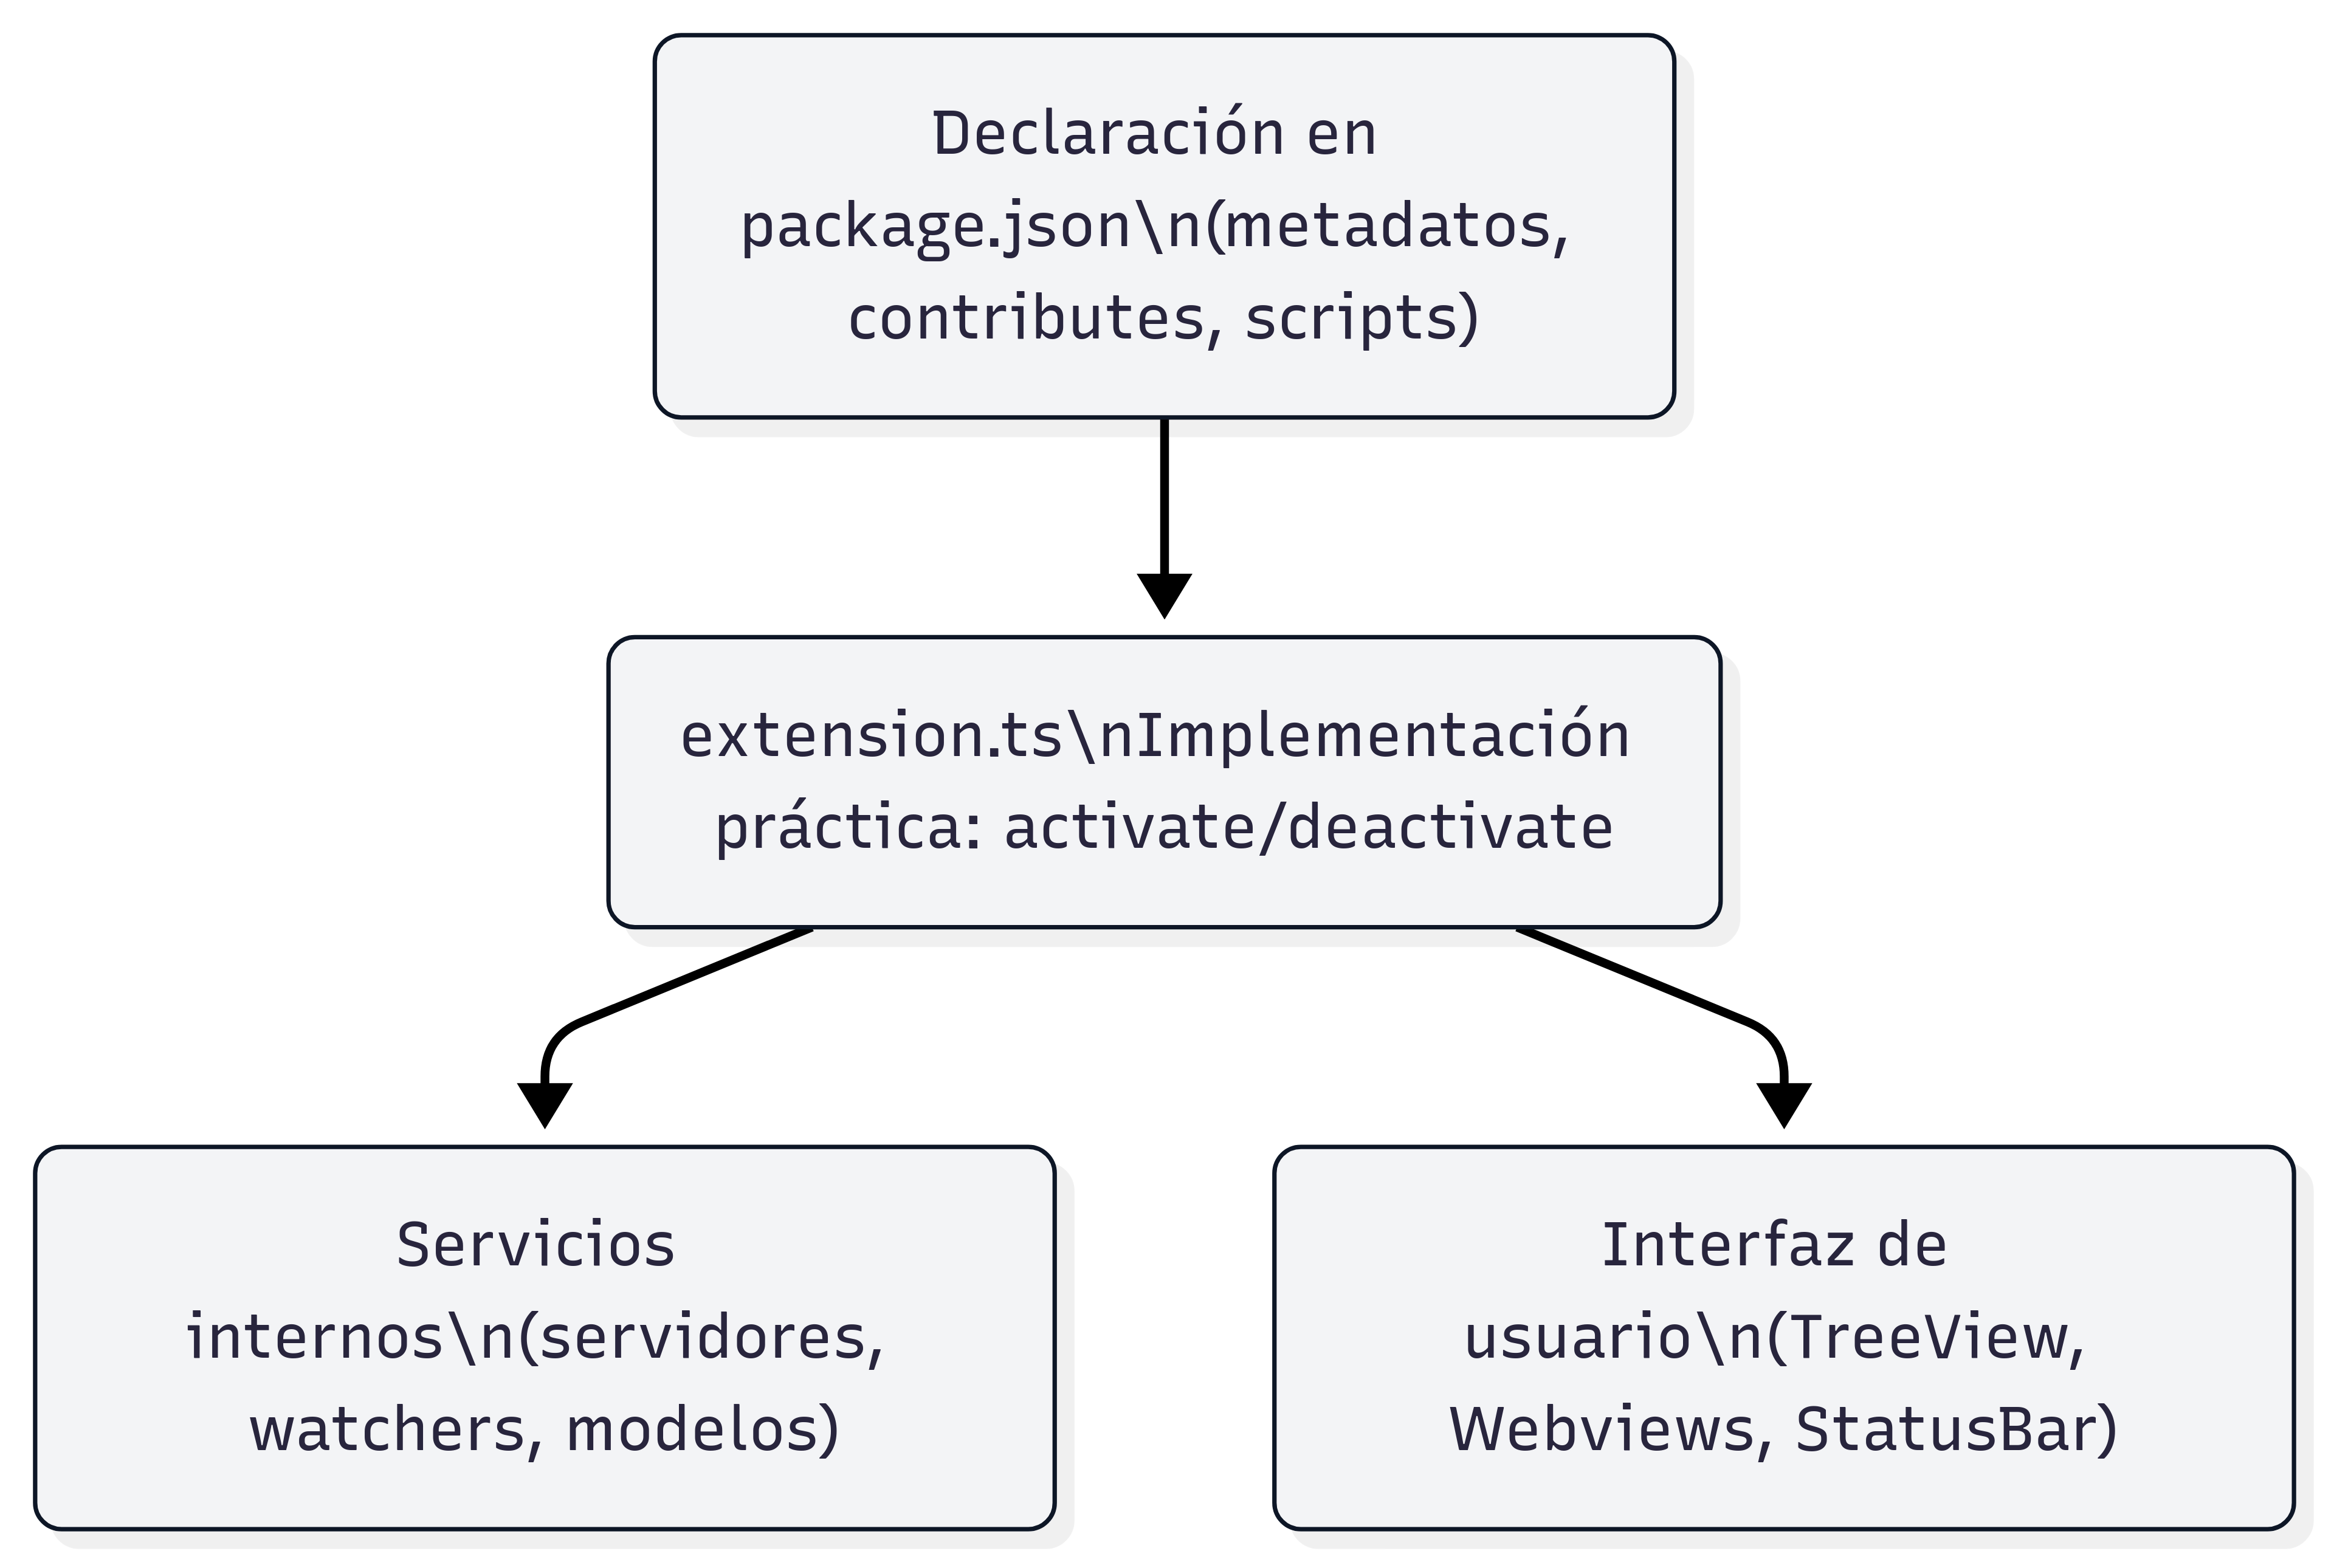
\includegraphics[width=0.8\linewidth]{img/fig-extension-structure.png}
\caption{Relación entre los componentes clave de una extensión VS Code en Code-XR.}
\label{fig:extension-structure}
\end{figure}

% SECCION DE SPRINTS

\section{Sprint 1 — Lanzamiento de servidores locales}
\label{sec:sprint-servers}

Este sprint estableció la capacidad fundamental de Code-XR para lanzar servidores locales, permitiendo servir visualizaciones XR desde el propio editor. La solución se inspiró en extensiones como \emph{Live Server}\cite{liveserver}, eliminando la necesidad de configurar servidores externos manualmente.

El subsistema de servidores proporciona \textbf{arquitectura modular}, \textbf{persistencia de preferencias}, \textbf{multi-servidor concurrente}, \textbf{resolución automática de puertos}, \textbf{soporte HTTP/HTTPS completo} y \textbf{gestión centralizada de estado}. El diseño sigue patrones escalables con separación de responsabilidades y gestión automatizada del ciclo de vida\cite{code-xr}.

\subsection{Arquitectura modular del subsistema}
El código se estructura en capas especializadas bajo \texttt{src/servers/} y \texttt{src/active\_servers/}, implementando una arquitectura de responsabilidades distribuidas:

\begin{itemize}
  \item \textbf{runtime}: Núcleo de ejecución con servidores HTTP/HTTPS, gestión de puertos y subsistema SSE.
  \item \textbf{storage}: Persistencia con validación atómica y migraciones de esquema.
  \item \textbf{registry}: Estado centralizado con eventos síncronos para UI.
  \item \textbf{services}: Validación de registros y control de WebviewPanels.
  \item \textbf{views}: Integración con TreeView de VS Code.
\end{itemize}

\subsection{Configuración y persistencia}
El \texttt{ServerSettingsManager} gestiona preferencias mediante \texttt{server-settings.json} en \texttt{globalStorage}, garantizando persistencia cross-workspace. El panel de configuración (Figura~\ref{fig:ui-server-config}) ofrece controles granulares: selección de protocolo HTTP/HTTPS con validación automática de certificados, configuración de puerto por defecto con detección de colisiones, apertura automática configurable y selección entre modo navegador o panel lateral. Los botones de acción directa permiten lanzar servidores con la configuración activa o restaurar valores por defecto.

\begin{figure}[H]
\centering
\begin{minipage}{0.9\linewidth}
\begin{lstlisting}[language=json,
caption={Configuración de servidores en Code-XR.},
label={fig:server-settings-json}]
{
  "mode": "HTTPS",
  "https": { "certSource": "default",
             "certPath": "certs/babia_cert.pem",
             "keyPath":  "certs/babia_key.pem" },
  "defaultPort": 3000,
  "launch": { "autoOpen": true, "openMode": "browser" },
  "configNonce": "37a3047821ba23de99348bcba2d155c3",
  "version": "1.0.0"
}
\end{lstlisting}
\end{minipage}
\end{figure}

\begin{figure}[H]
\centering
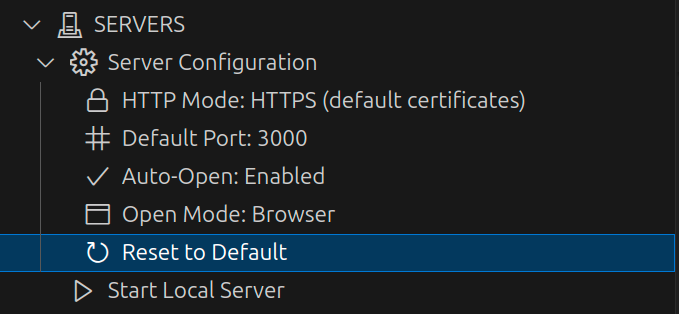
\includegraphics[width=0.65\linewidth]{img/ui-server-config.png}
\caption{Panel de configuración avanzada con controles HTTP/HTTPS, puertos y modo de lanzamiento.}
\label{fig:ui-server-config}
\end{figure}

\subsection{Gestión inteligente de puertos y HTTP/HTTPS}
El \texttt{PortManager} implementa descubrimiento automático mediante \texttt{get-port}\cite{get-port}, realizando búsqueda secuencial desde el puerto configurado hasta encontrar uno disponible. Ante colisiones, notifica transparentemente la reasignación.
Se soporta HTTP y HTTPS (obligatorio para XR); en caso de intentar usar HTTPS con panel lateral, el plugin avisa y fuerza el uso de HTTP por limitaciones de VS Code.
%Salto de linea

El soporte HTTPS ofrece dos modalidades:
\begin{itemize}
  \item \textbf{Certificados por defecto}: Par \texttt{cert/key} incluido, generados con \texttt{OpenSSL}\cite{openssl}.
  \item \textbf{Certificados personalizados}: Selector con validación de compatibilidad.
\end{itemize}

\subsection{Modos de visualización}
Code-XR ofrece dos modos de visualización de los servidores lanzados, configurables desde el panel de settings:

\begin{figure}[H]
\centering
\begin{minipage}[b]{0.48\textwidth}
\centering
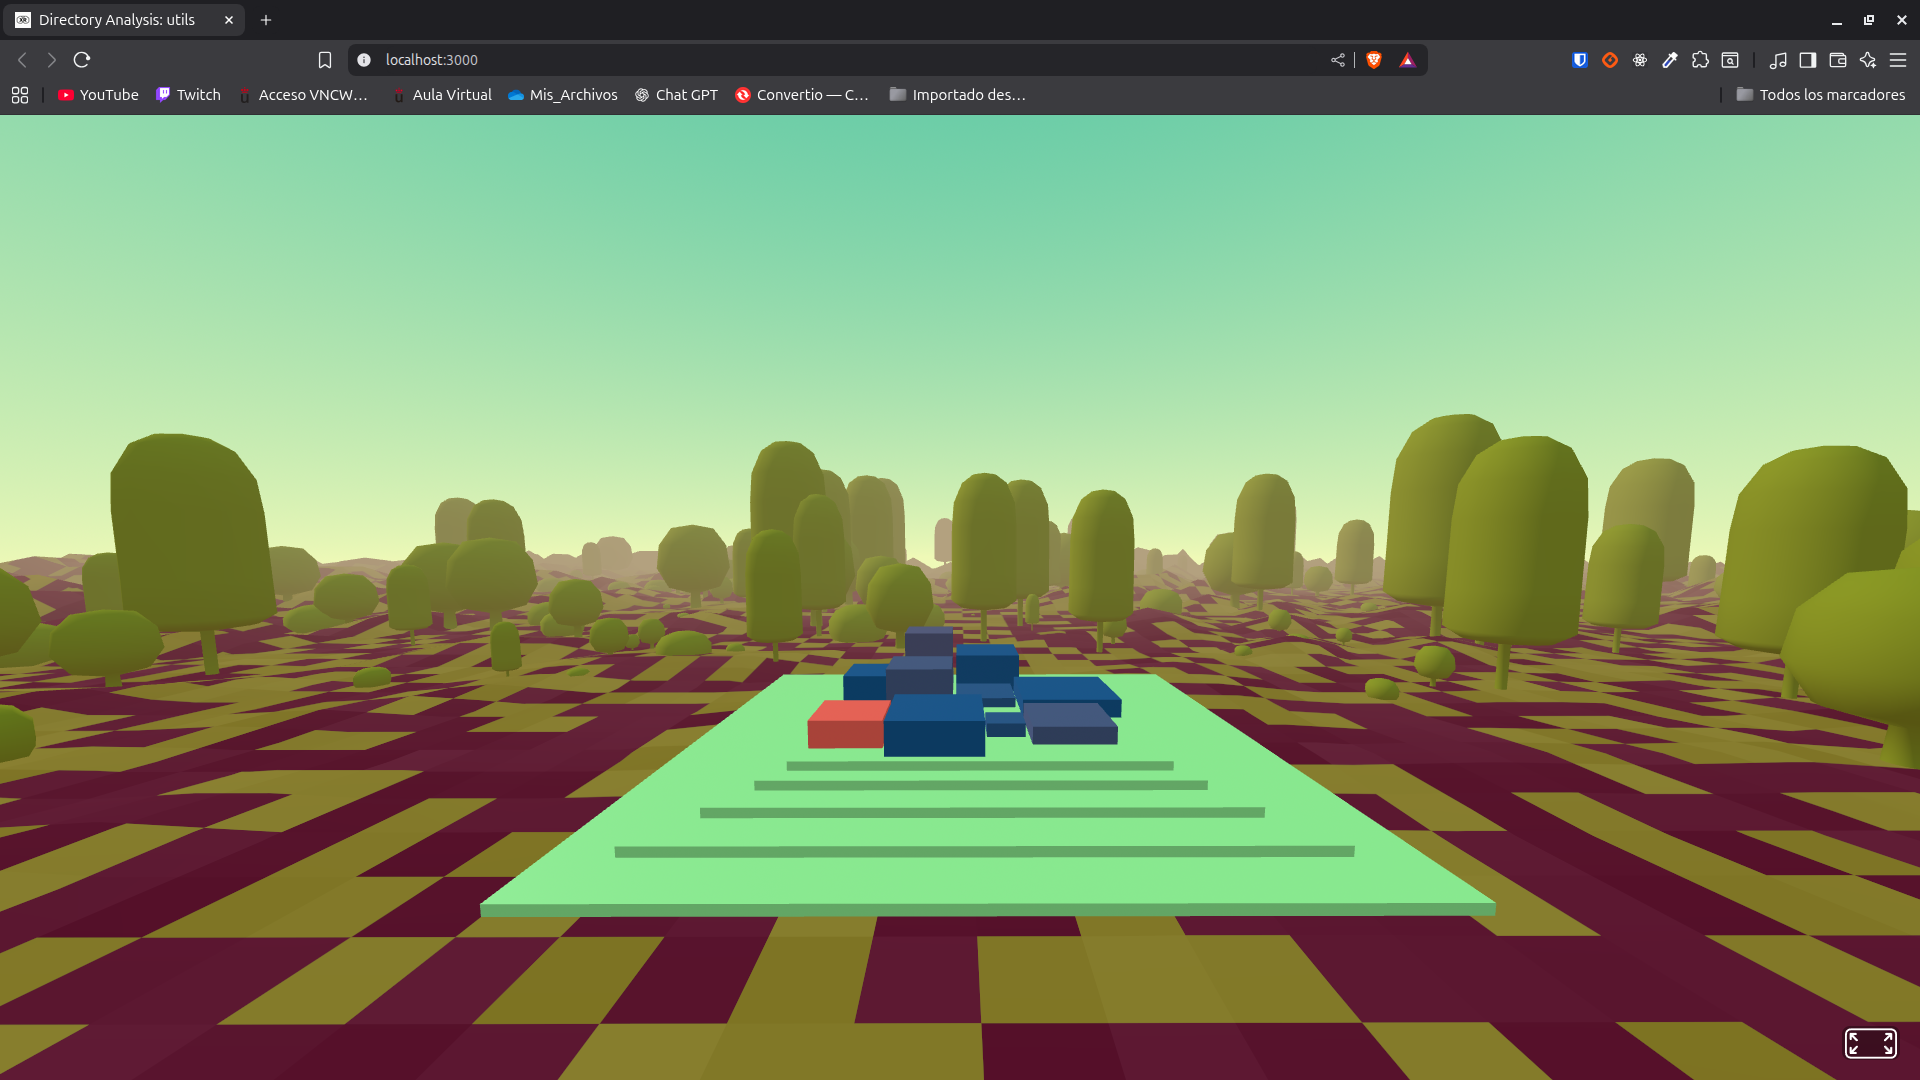
\includegraphics[width=\textwidth]{img/browser-mode.png}
\subcaption{Modo navegador: visualización completa en navegador web externo}
\end{minipage}
\hfill
\begin{minipage}[b]{0.48\textwidth}
\centering
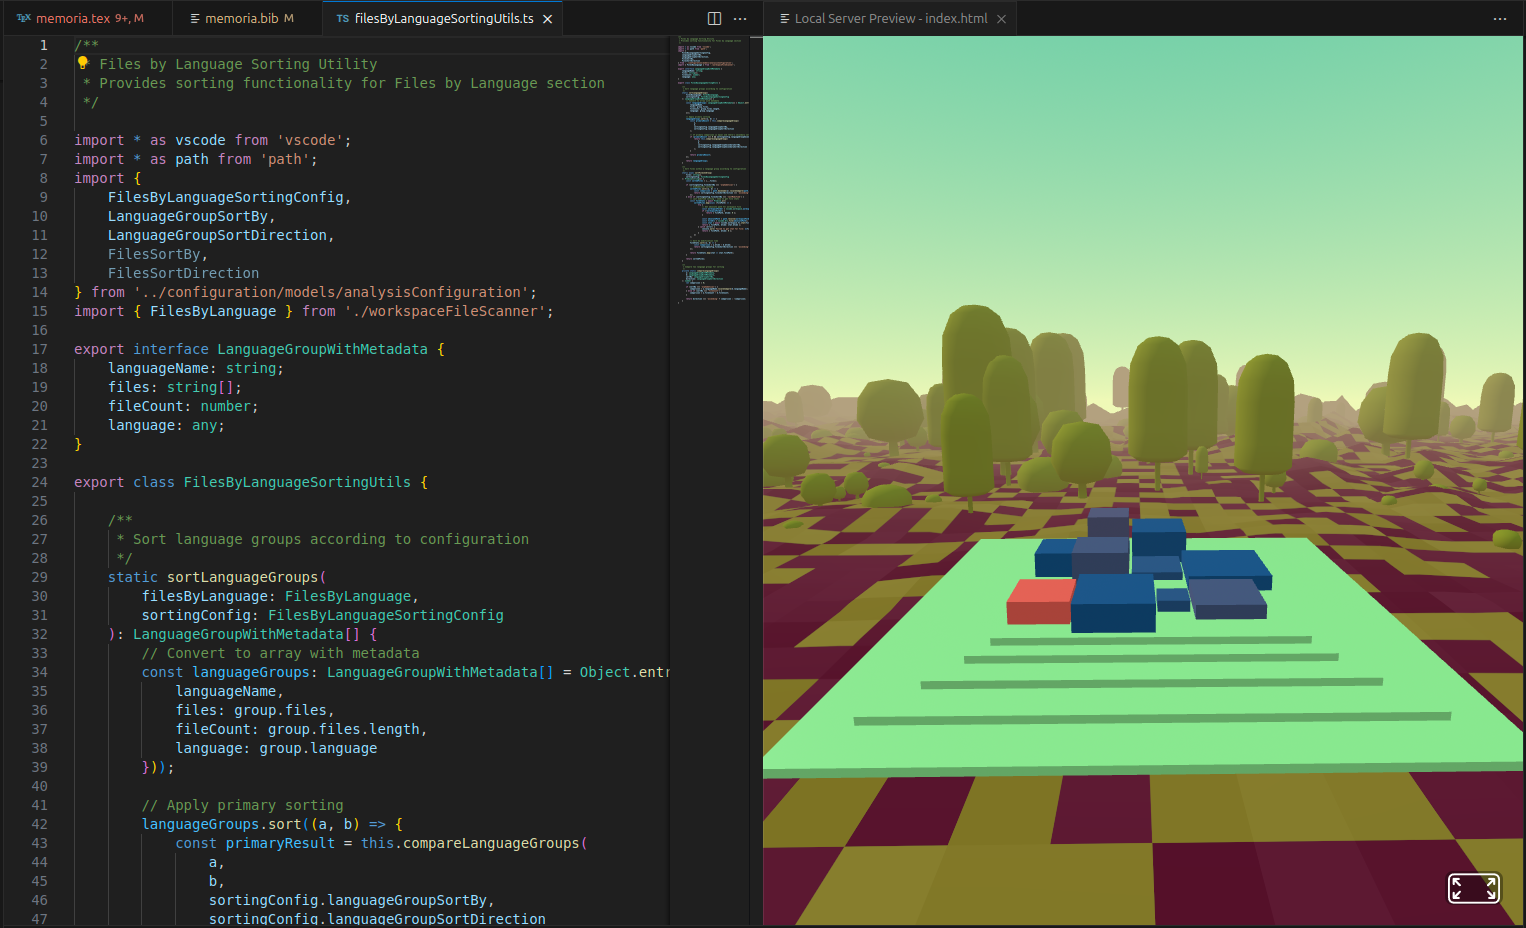
\includegraphics[width=\textwidth]{img/panel-mode.png}
\subcaption{Modo panel lateral: integración directa en VS Code}
\end{minipage}
\caption{Comparación entre los dos modos de visualización: navegador web (izquierda) y panel lateral integrado (derecha).}
\label{fig:visualization-modes}
\end{figure}
\textbf{Nota:} Ambas imágenes muestran el mismo análisis XR del directorio \texttt{src/utils} de Code-XR.

\subsection{Active Servers y observabilidad}
La vista \emph{Active Servers} expone un registro centralizado que rastrea instancias activas con estado completo, metadatos contextuales y acciones específicas. El registro es efímero para prevenir servidores zombie y garantizar coherencia entre sesiones.

Esta vista presenta un registro en tiempo real con información completa de cada instancia: identificador único, puerto asignado, URL de acceso, modo de lanzamiento y estado operacional (Para acceder a la información click izquierdo en el elemento que se desee). Las acciones contextuales incluyen apertura en navegador, copia de URL, visualización de detalles técnicos y parada individual o masiva de servidores.

\begin{figure}[H]
\centering
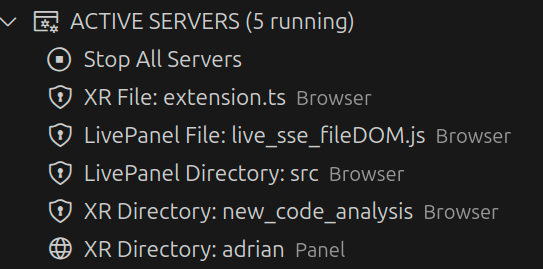
\includegraphics[width=0.65\linewidth]{img/ui-active-servers.png}
\caption{Vista \emph{Active Servers} con registro centralizado y acciones contextuales.}
\label{fig:ui-active-servers}
\end{figure}

\subsection{Comunicación en tiempo real (SSE)}
Los servidores exponen endpoints \texttt{/events} con \emph{Server-Sent Events} para propagación automática de cambios de análisis, gestión de clientes y mapeo archivo-servidor. El sistema actúa como bus de comunicación entre extensión y visualizaciones web.

\subsection{Compatibilidad VR}
\texttt{NetworkUtils} detecta automáticamente la IP local y genera URLs de acceso externo, facilitando uso desde dispositivos VR en la misma red mediante bind a \texttt{0.0.0.0}.

%----------------------------------------------------------------
% Sprint 2 - BabiaXR
%----------------------------------------------------------------

\section{Sprint 2 — Integración con BabiaXR y ejemplos de visualización}
\label{sec:sprint-babiaxr}

Este sprint estableció las capacidades de visualización XR completas de Code-XR mediante la integración con \textbf{BabiaXR}, motor de visualización 3D para todas las representaciones WebXR/AR/VR del plugin. El desarrollo siguió tres fases consecutivas para dominar la integración entre \textbf{BabiaXR}, \textbf{datos JSON} y el \textbf{plugin VS Code}, preparando el Sprint 3 de análisis en tiempo real.

\textbf{Fase 1: Comprensión mediante ejemplos} — Galería de ejemplos predefinidos basados en BabiaXR\cite{babiaxr-examples} para familiarización con tipos de gráficos, configuración y estructuras de datos.

\textbf{Fase 2: Pipeline JSON→XR} — Transformación automática de ficheros JSON en visualizaciones XR mediante análisis de estructura, mapeo de dimensiones y generación de plantillas HTML/A-Frame.

\textbf{Fase 3: Personalización visual} — Control granular de aspectos estéticos: ambientes XR, colores de fondo/suelo y paletas cromáticas aplicables tanto a datos JSON como análisis de código.

\paragraph{Módulos resultantes}
\begin{enumerate}
  \item \textbf{Babia Examples}: galería interactiva de ejemplos BabiaXR con lanzamiento directo y gestión centralizada.
  \item \textbf{Visualize Data}: pipeline JSON→XR con análisis automático, mapeo inteligente y validación contextual.
  \item \textbf{Visualization Settings}: configuración visual global para entornos, colores y paletas aplicada a todas las visualizaciones.
\end{enumerate}

Todos reutilizan la infraestructura de servidores del Sprint 1, garantizando coherencia en comportamiento, configuración y experiencia de usuario.



%---------------------------
% Babia Examples
%---------------------------

\subsection{Babia Examples}
\label{sec:babia-examples}

El subsistema \emph{Babia Examples} proporciona una galería interactiva de ejemplos predefinidos BabiaXR dentro de VS Code, facilitando el acceso inmediato a visualizaciones WebXR/AR/VR mediante un flujo de un clic. Permite explorar capacidades de BabiaXR, experimentar con diferentes gráficos y usar ejemplos como plantillas de referencia\cite{babiaxr-examples}.

Reutiliza la infraestructura de servidores del Sprint~\ref{sec:sprint-servers}, lanzando ejemplos según la configuración activa y registrándolos en \emph{Active Servers} para gestión centralizada.

\paragraph{Arquitectura y descubrimiento}
Implementa arquitectura modular bajo \texttt{src/babia\_examples/} con capas especializadas: \texttt{model/}, \texttt{runtime/}, \texttt{views/} y \texttt{commands/}. El \texttt{ExampleLauncher} busca automáticamente ejemplos disponibles recorriendo \texttt{examples/charts/} y detectando archivos HTML válidos.

\paragraph{Catálogo de ejemplos}
La colección incluye gráficos diversos que ilustran técnicas BabiaXR:

\begin{itemize}
  \item \textbf{Bar Chart}: gráfico de barras clásico en dos ejes.
  \item \textbf{Barsmap}: variante espacial con tres ejes.
  \item \textbf{Bubble Chart}: dispersión 3D con tamaño como cuarto eje.
  \item \textbf{Cylinder Chart}: bar chart con cilindros tridimensionales.
  \item \textbf{Cylindermap Chart}: barsmap con cilindros.
  \item \textbf{Pie}: gráfico circular clásico.
  \item \textbf{Mix}: escenario combinando cuatro tipos de gráficos.
\end{itemize}

\begin{figure}[H]
\centering
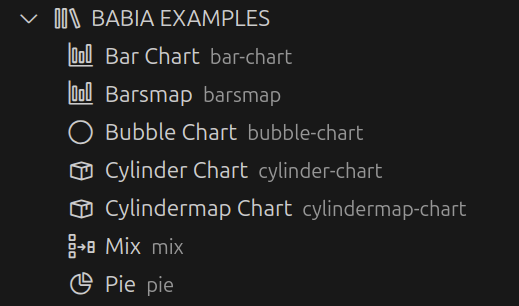
\includegraphics[width=0.55\linewidth]{img/ui-babia-examples.png}
\caption{Vista del apartado \emph{Babia Examples} mostrando la galería de ejemplos BabiaXR disponibles, cada uno lanzable con un clic y con integración completa en el ecosistema de servidores de Code-XR.}
\label{fig:ui-babia-examples}
\end{figure}

\paragraph{Integración ecosistémica}
Sigue principios de delegación inteligente, aprovechando la infraestructura existente sin duplicar funcionalidad. Delega al \texttt{MultiServerLauncher} para garantizar comportamiento consistente en puertos, certificados SSL y registro en \emph{Active Servers}. Los ejemplos aparecen con nombres descriptivos y heredan preferencias de configuración.

\paragraph{Estructura de archivos}
El directorio \texttt{examples/} separa recursos y datos:
\begin{itemize}
  \item \texttt{charts/}: estructura categórica con ejemplos HTML completos.
  \item \texttt{data/}: datasets centralizados (\texttt{gdp.json}, \texttt{population.json}, etc.) para demostraciones.
\end{itemize}

Esta organización facilita reutilización, mantenimiento y escalabilidad para nuevos ejemplos.

%---------------------------
% Visualize Data
%---------------------------

\subsection{Visualize Data — del JSON a una visualización XR}
\label{sec:visualize-data}

El subsistema \emph{Visualize Data} constituye el núcleo de transformación de datos, proporcionando un pipeline que convierte ficheros \texttt{JSON} arbitrarios en visualizaciones inmersivas BabiaXR mediante un flujo guiado de cuatro etapas: selección de gráfico, análisis JSON, mapeo de dimensiones y lanzamiento. Se integra transparentemente con la infraestructura del Sprint~\ref{sec:sprint-servers} y hereda automáticamente preferencias de \emph{Visualization Settings}.

\paragraph{Arquitectura modular}
Implementa arquitectura distribuida bajo \texttt{src/visualize\_data/} con capas especializadas: \texttt{state/}, \texttt{model/}, \texttt{runtime/}, \texttt{commands/} y \texttt{views/}. El estado se persiste a nivel workspace, garantizando configuraciones persistentes entre sesiones.

\paragraph{Catálogo de gráficos}
Incluye tipos BabiaXR: \emph{Bar}, \emph{Pie}, \emph{Donut}, \emph{Bubbles}, \emph{Cylinders}, \emph{Barsmap}, \emph{Cylindermap}, \emph{Mix} y \emph{Boats}. Cada tipo define dimensiones específicas y plantilla HTML/BabiaXR asociada, estableciendo las bases para el análisis de código.

\begin{figure}[H]
\centering
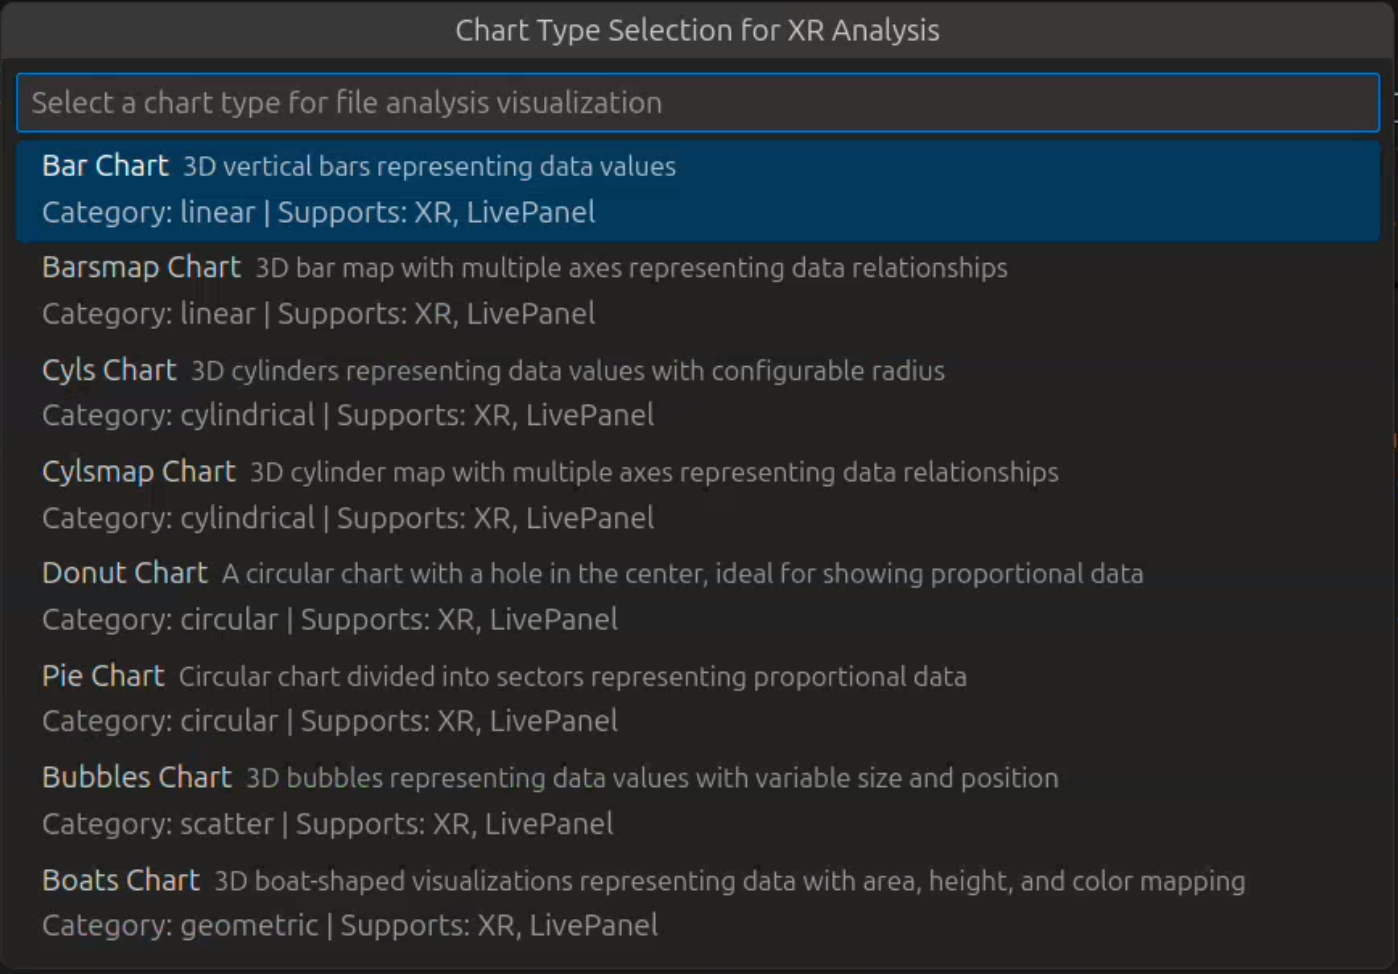
\includegraphics[width=0.58\linewidth]{img/graficos_babiaxr.png}
\caption{Selector de gráficos disponibles en \emph{Visualize Data}, mostrando la diversidad de tipos de visualización BabiaXR soportados.}
\label{fig:visualize-chart-selector}
\end{figure}

\paragraph{Análisis inteligente JSON}
El analizador identifica estructura y clasifica valores entre numéricos y no numéricos (\emph{string}, \emph{boolean}, \emph{object}, \emph{array}), considerando que ciertos ejes BabiaXR requieren datos numéricos exclusivamente. Genera resumen estructurado con entradas totales, tipos de campo y ejemplos de valores.

\paragraph{Mapeo de dimensiones contextual}
Permite asignar campos JSON a dimensiones gráficas con validación inteligente: dimensiones numéricas (\texttt{size}, \texttt{height}) filtran automáticamente campos disponibles. Proporciona retroalimentación en tiempo real, validación de coherencia y prevención de configuraciones incompletas.

\begin{figure}[H]
\centering
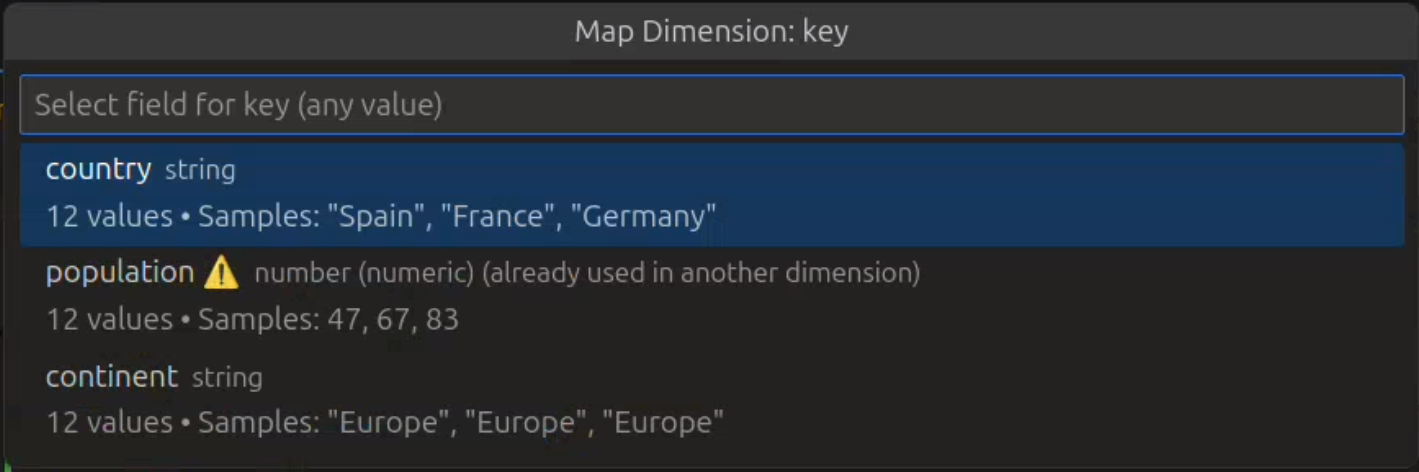
\includegraphics[width=0.80\linewidth]{img/ui-dimension-mapping-process.png}
\caption{Interfaz de mapeo de dimensiones con validación contextual, mostrando la asignación de campos JSON a dimensiones del gráfico con filtrado por tipo de dato.}
\label{fig:ui-dimension-mapping-process}
\end{figure}

\paragraph{Generación y persistencia}
Combina plantilla HTML del gráfico con datos mapeados y preferencias globales de \emph{Visualization Settings}, inyectando automáticamente paleta cromática, ambiente XR y configuración de suelo. Almacena visualizaciones en \texttt{globalStorage} con directorios únicos (\texttt{Identificador\_{nonce}}) conteniendo \texttt{index.html} y \texttt{data.json}.

\paragraph{Browse Visualizations}
Gestiona biblioteca personal de visualizaciones: escanea \texttt{globalStorage}, valida integridad de archivos y ofrece relanzamiento individual o limpieza masiva (\emph{Reset All}). Transforma el subsistema en herramienta reutilizable con integración completa al sistema de servidores.

\begin{figure}[H]
\centering
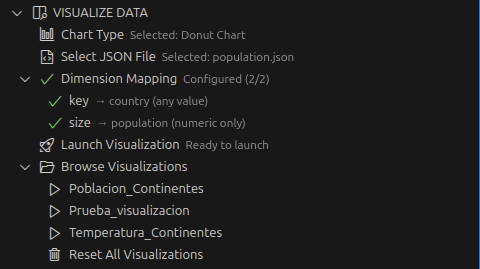
\includegraphics[width=0.70\linewidth]{img/ui-visualize-data.png}
\caption{Interfaz completa de \emph{Visualize Data} mostrando el flujo de trabajo paso a paso y la gestión de biblioteca de visualizaciones almacenadas.}
\label{fig:ui-visualize-data}
\end{figure}

\paragraph{Integración ecosistémica}
Delega lanzamiento al \texttt{MultiServerLauncher} siguiendo la arquitectura del Sprint~\ref{sec:sprint-servers}, garantizando consistencia en HTTP/HTTPS, puertos automáticos y registro en \emph{Active Servers}. La herencia automática desde \emph{Visualization Settings} aplica configuración estética consistente sin intervención del usuario.


%---------------------------
% Visualization Settings
%---------------------------

\subsection{Visualization Settings}
\label{sec:visualization-settings}

El apartado \emph{Visualization Settings} constituye el sistema de configuración visual global, permitiendo personalizar cuatro aspectos fundamentales aplicados automáticamente a todas las visualizaciones: \textbf{color de fondo}, \textbf{color del suelo}, \textbf{preset del entorno} y \textbf{paleta de gráficos}.

\paragraph{Arquitectura y persistencia}
Sigue la arquitectura modular establecida bajo \texttt{src/visualization\_settings/} con separación entre \texttt{model/}, \texttt{storage/}, \texttt{commands/}, \texttt{views/} y \texttt{utils/}. 

Implementa persistencia dual: \texttt{visualization-settings.json} en \texttt{globalStorage} (primario) y \texttt{globalState} (respaldo), garantizando configuraciones cross-workspace con migración automática.

\begin{figure}[H]
\centering
\begin{minipage}{0.9\linewidth}
\begin{lstlisting}[language=json,
caption={Estructura del archivo \texttt{visualization-settings.json} que persiste las preferencias visuales globales.},
label={fig:visualization-settings-json}]
{
  "backgroundColor": "#FFFFFF",
  "groundColor": "#000000",
  "environment": "forest", 
  "palette": "ubuntu"
}
\end{lstlisting}
\end{minipage}
\end{figure}

\paragraph{Interfaz visual integrada}
Se presenta como apartado colapsible en el árbol principal con iconografía contextual: \emph{Background/Ground Color} muestran iconos SVG dinámicos de 16×16 píxeles reflejando el color seleccionado, mientras \emph{Environment Preset} y \emph{Chart Palette} muestran texto de la opción activa.

% TODO: Capturar screenshot del apartado Visualization Settings en el árbol de Code-XR 
% mostrando los 4 elementos con sus iconos dinámicos de color
% Nombre sugerido: ui-visualization-settings-tree.png
\begin{figure}[H]
\centering
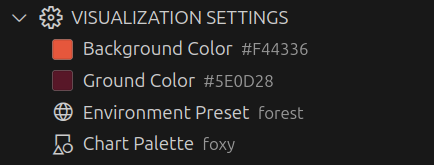
\includegraphics[width=0.60\linewidth]{img/ui-visualization-settings-tree.png}
\caption{Vista del apartado \emph{Visualization Settings} integrado en el árbol principal, mostrando iconos dinámicos de color para los parámetros visuales.}
\label{fig:ui-visualization-settings-tree}
\end{figure}

\paragraph{Configuración de colores}
Implementa flujo híbrido con webview personalizado integrando selector HTML5 nativo, proporcionando preview en tiempo real y validación automática hexadecimal (\texttt{\#RRGGBB}).

% TODO: Capturar screenshot del panel de selección de colores (webview) 
% mostrando el color picker HTML5 con el color actual seleccionado
% Nombre sugerido: ui-color-picker-panel.png
\begin{figure}[H]
\centering
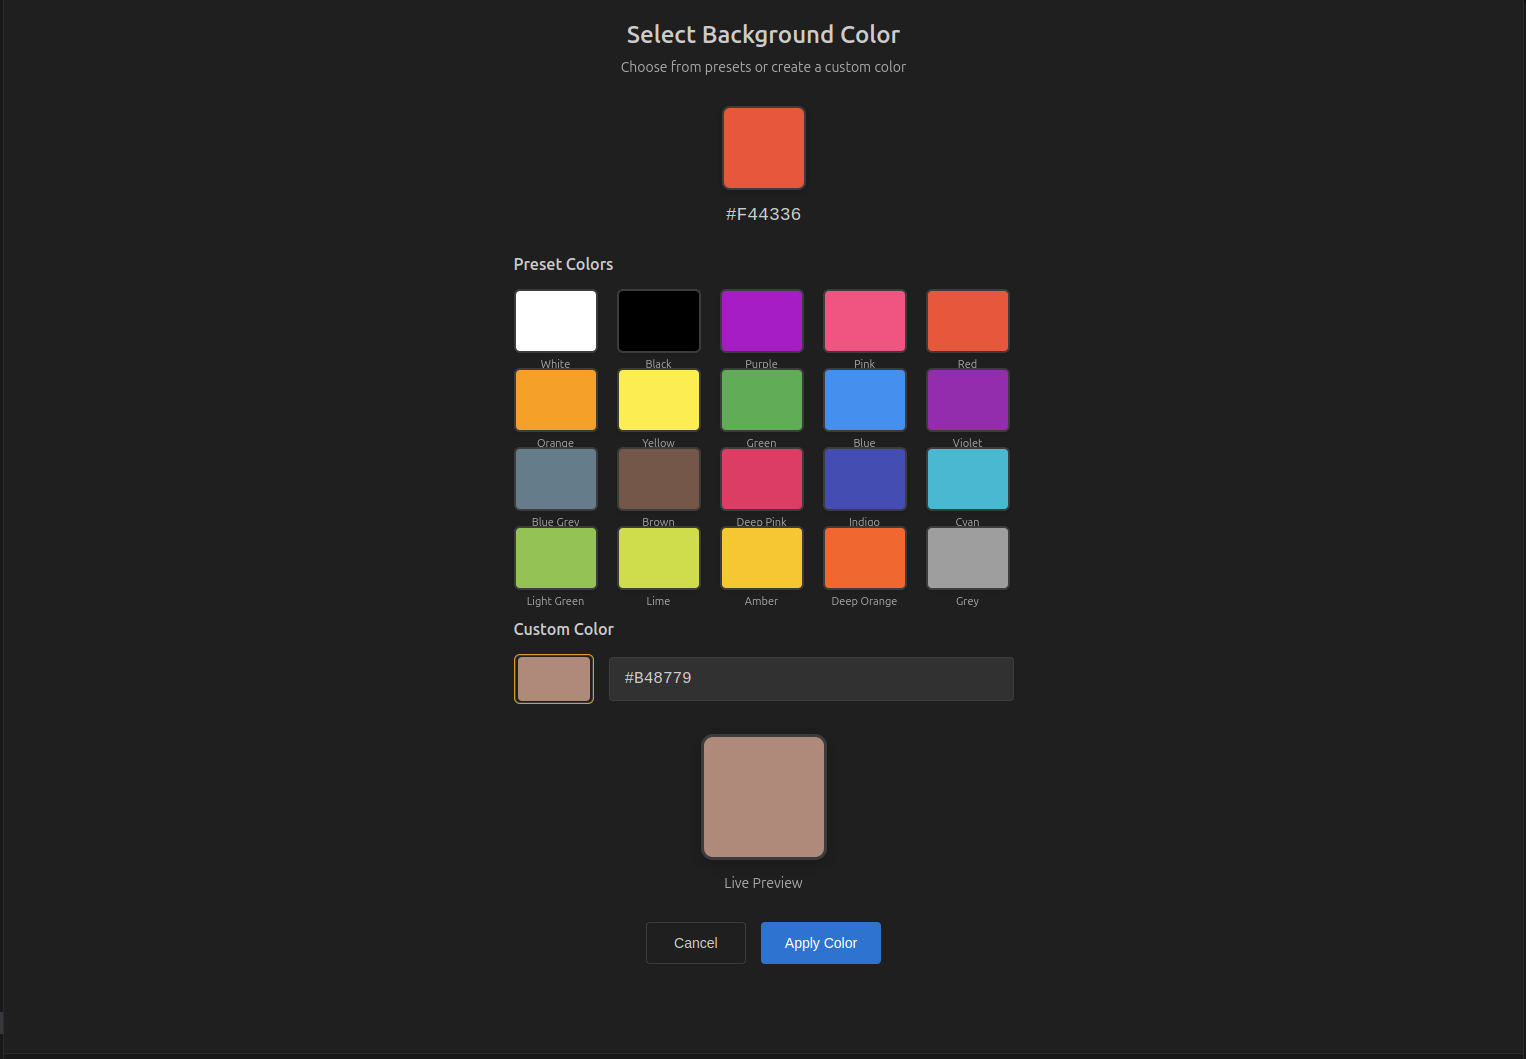
\includegraphics[width=1\linewidth]{img/ui-color-picker-panel.png}
\caption{Panel de selección de colores mediante webview integrado, utilizando el selector HTML5 nativo con validación en tiempo real.}
\label{fig:ui-color-picker-panel}
\end{figure}


\paragraph{Entornos y paletas}
Utiliza interfaz \emph{QuickPick} para selección contextual. Entornos: 12 presets A-Frame (\texttt{forest}, \texttt{tron}, \texttt{egypt}, \texttt{dream}, \texttt{volcano}, \texttt{arches}, etc.) redefiniendo ambientación XR completa. Paletas: 9 esquemas cromáticos BabiaXR (\texttt{ubuntu}, \texttt{blues}, \texttt{sunset}, \texttt{foxy}, \texttt{icecream}, etc.) optimizados por contexto.

% TODO: Capturar screenshot de los QuickPick de Environment Preset y Chart Palette
% mostrando la lista de entornos y paletas disponibles
% Nombre sugerido: ui-environment-chart-quickpicks.png
\begin{figure}[H]
\centering
\begin{minipage}[b]{0.48\textwidth}
\centering
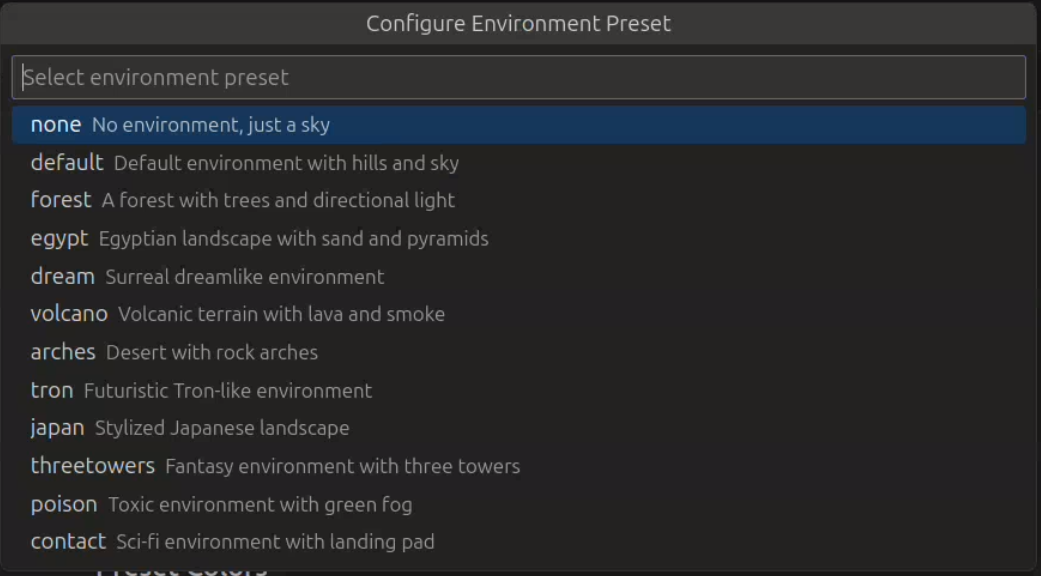
\includegraphics[width=\textwidth]{img/ui-environment-preset-quickpick.png}
\subcaption{Selector \emph{QuickPick} para \emph{Environment Preset}}
\end{minipage}
\hfill
\begin{minipage}[b]{0.48\textwidth}
\centering
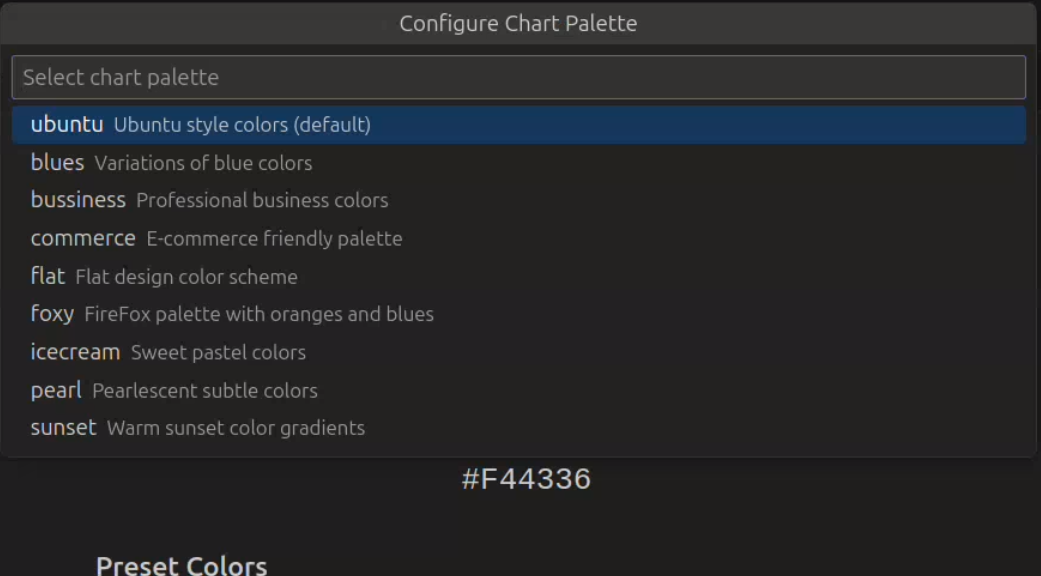
\includegraphics[width=\textwidth]{img/ui-chart-palette-quickpick.png}
\subcaption{Selector \emph{QuickPick} para \emph{Chart Palette}}
\end{minipage}
\caption{Selectores \emph{QuickPick} para configuración visual: entornos A-Frame disponibles con descripciones contextuales (izquierda) y paletas de colores BabiaXR con vistas previas (derecha).}
\label{fig:ui-quickpick-selectors}
\end{figure}

\paragraph{Aplicación automática}
Integración transparente con motor de plantillas: \texttt{getVisualizationConfiguration()} recupera preferencias e inyecta en plantillas HTML/A-Frame. Mapeo directo:
\begin{itemize}
\item \textbf{Background Color} $\rightarrow$ atributo \texttt{background="color: \#FFFFFF"} de la escena A-Frame
\item \textbf{Environment Preset} $\rightarrow$ componente \texttt{environment="preset: forest"} 
\item \textbf{Ground Color} $\rightarrow$ parámetro \texttt{groundColor: \#000000} del entorno
\item \textbf{Chart Palette} $\rightarrow$ atributo \texttt{palette: ubuntu} en componentes BabiaXR
\end{itemize}

\paragraph{Iconografía dinámica}
Generación automática de iconos SVG como indicadores visuales: cuadrados 16×16 píxeles para colores, efectos de borde para legibilidad en temas VS Code, nomenclatura \texttt{\{settingKey\}\_\{hexcolor\}.svg} con caché eficiente y limpieza automática de obsoletos.

\subsection{Integración de fases y transición al Sprint 3}
Esta aproximación incremental estableció una base arquitectónica sólida y extensible que permitió avanzar hacia el analizador y visualizador de análisis en tiempo real del siguiente sprint. Cada fase aportó componentes modulares reutilizables, garantizando que Code-XR cumpliera objetivos funcionales con experiencia de usuario fluida.

%----------------------------------------------------------------
% Sprint 3 - Analizador y visualizador de análisis de código
%----------------------------------------------------------------
\section{Sprint 3 — Análisis y visualización de métricas de código}

\subsection{Introducción al análisis de código}
\label{sec:intro-analisis}

El subsistema de análisis de código constituye el núcleo de Code-XR, transformando código fuente en visualizaciones interactivas 2D y XR. Integra los componentes desarrollados en sprints anteriores para ofrecer comprensión intuitiva de la estructura y complejidad del software.

\paragraph{Contexto y evolución desde sprints anteriores}
Aprovecha componentes clave de sprints anteriores:

\begin{itemize}
  \item \textbf{Sprint 1 — Infraestructura de servidores}: arquitectura modular HTTP/HTTPS para alojar visualizaciones dinámicas y gestionar múltiples sesiones.
  \item \textbf{Sprint 2 — Visualización con BabiaXR}: plantillas BabiaXR y sistema de configuración para visualizaciones personalizadas.
\end{itemize}

\paragraph{Capacidades principales del subsistema}  
Dos ejes fundamentales: \emph{alcance} y \emph{modo de visualización}.

\begin{enumerate}
  \item \textbf{Alcance del análisis}:
    \begin{itemize}
      \item \textbf{Análisis de fichero individual}: métricas detalladas (complejidad, distribución código/comentarios, estructura de clases).
      \item \textbf{Análisis de directorio}: agregación multi-archivo, distribución de lenguajes y complejidad global.
      \item \textbf{Análisis de proyecto}: visión holística incluyendo dependencias y estructura organizativa.
    \end{itemize}
  
  \item \textbf{Modos de visualización}:
    \begin{itemize}
      \item \textbf{LivePanel}: visualización 2D integrada en VS Code mediante webviews.
      \item \textbf{XR Mode}: representación tridimensional inmersiva para entornos VR/AR.
      \item \textbf{DOM Mode}: visualización especializada de estructura DOM como árbol 3D interactivo.
    \end{itemize}
    
\end{enumerate}

\begin{figure}[H]
\centering
\begin{tikzpicture}[
    node distance=1.5cm, 
    block/.style={rectangle, draw, fill=gray!10, minimum width=2.5cm, minimum height=1cm, align=center}
]

% Core Analysis System
\node[block, fill=blue!20] (core) {Subsistema \\ de Análisis};

% Analysis Modes
\node[block, above of=core, xshift=-2.5cm] (file) {Fichero};
\node[block, above of=core] (dir) {Directorio};
\node[block, above of=core, xshift=2.5cm] (proj) {Proyecto};

% Visualization Modes
\node[block, below of=core, xshift=-2.5cm] (live) {LivePanel};
\node[block, below of=core] (xr) {XR};
\node[block, below of=core, xshift=2.5cm] (dom) {DOM};

% Connections
\draw[-latex] (file) -- (core);
\draw[-latex] (dir) -- (core);
\draw[-latex] (proj) -- (core);
\draw[-latex] (core) -- (live);
\draw[-latex] (core) -- (xr);
\draw[-latex] (core) -- (dom);

\end{tikzpicture}
\caption{Dimensiones fundamentales del subsistema de análisis: alcance del análisis (entrada) y modos de visualización (salida).}
\label{fig:analisis-dimensiones}
\end{figure}

\paragraph{Objetivos técnicos y de experiencia de usuario}
Objetivos clave del subsistema:

\begin{itemize}
  \item \textbf{Análisis en tiempo real}: retroalimentación instantánea sobre cambios en el código.
  \item \textbf{Representación intuitiva}: transformar conceptos abstractos en metáforas visuales comprensibles.
  \item \textbf{Escalabilidad}: rendimiento óptimo con proyectos grandes mediante análisis incremental.
  \item \textbf{Integración fluida}: fusión con el flujo natural de trabajo en VS Code.
  \item \textbf{Personalización}: adaptación según preferencias específicas del usuario.
  \item \textbf{Extensibilidad}: facilitar adición de nuevos analizadores y visualizaciones.
\end{itemize}

En las siguientes secciones se detalla la arquitectura técnica, el flujo de datos, los motores de análisis y los mecanismos de visualización que hacen posible esta funcionalidad.

\subsection{Arquitectura del subsistema de análisis}
\label{sec:arquitectura-analisis}

El subsistema implementa una arquitectura modular combinando patrones de diseño para flexibilidad, mantenibilidad y rendimiento en análisis múltiples, sesiones simultáneas y actualizaciones en tiempo real.

\paragraph{Patrones de diseño aplicados}
Patrones clave para organización y extensibilidad:

\begin{itemize}
  \item \textbf{Patrón "Nested Dolls"}: registro de comandos donde cada subsistema contribuye sin conocimiento de otros componentes (principio Matryoshka).
  \item \textbf{Patrón Registry}: \texttt{UnifiedSessionRegistry} como punto central para gestión del ciclo de vida de sesiones.
  \item \textbf{Patrón Observer}: sistema de \emph{watchers} que monitoriza cambios y emite eventos SSE para actualizaciones en tiempo real.
  \item \textbf{Patrón Factory}: fábricas especializadas como \texttt{NewCodeAnalysisItemFactory} para generar implementaciones concretas.
\end{itemize}

\paragraph{Componentes principales}
La arquitectura está organizada en componentes especializados con responsabilidades bien definidas:

\begin{enumerate}
  \item \textbf{Analysis Orchestrator}: coordina proceso completo desde solicitud hasta visualización.
  \item \textbf{Session Registry}: registro centralizado de sesiones activas con estado y configuración.
  \item \textbf{Python Engine}: extrae métricas del código fuente mediante bibliotecas especializadas.
  \item \textbf{File Requirement Processor}: prepara archivos necesarios (plantillas HTML, scripts JS/CSS, datos).
  \item \textbf{Template Engine}: combina plantillas con datos de análisis y configuraciones visuales.
  \item \textbf{Session Watcher Manager}: gestiona observadores de archivos para re-análisis automáticos.
  \item \textbf{Session Server Manager}: controla servidores HTTP y canales SSE.
  \item \textbf{Configuration Storage}: almacena configuraciones, preferencias y perfiles de usuario.
\end{enumerate}

\begin{figure}[H]
\centering
\begin{tikzpicture}[
  node distance=2cm and 2.5cm,
  component/.style={rectangle, draw, fill=gray!10, minimum width=3.2cm, minimum height=1.2cm, align=center, font=\small},
  manager/.style={rectangle, draw, fill=blue!10, minimum width=3.2cm, minimum height=1.2cm, align=center, font=\small},
  engine/.style={rectangle, draw, fill=green!10, minimum width=3.2cm, minimum height=1.2cm, align=center, font=\small},
  storage/.style={cylinder, draw, shape border rotate=90, fill=yellow!10, minimum width=2.5cm, minimum height=1.5cm, align=center, font=\small},
  arrow/.style={thick,-latex, color=blue!60}
]

% Top layer - Main orchestrator
\node[component] (orchestrator) {Analysis\\Orchestrator};

% Second layer - Core engines
\node[manager, below left=of orchestrator] (session) {Session\\Registry};
\node[engine, below right=of orchestrator] (python) {Python\\Engine};

% Third layer - Processing components
\node[component, below=of session, xshift=-1.5cm] (require) {File Requirement\\Processor};
\node[component, below=of session, xshift=1.5cm] (template) {Template\\Engine};

% Fourth layer - Management components
\node[manager, below=of python, xshift=-1.5cm] (watcher) {Session Watcher\\Manager};
\node[manager, below=of python, xshift=1.5cm] (server) {Session Server\\Manager};

% Bottom layer - Storage
\node[storage, below=of template, yshift=-0.5cm] (config) {Configuration\\Storage};

% Main orchestration connections
\draw[arrow] (orchestrator) -- (session);
\draw[arrow] (orchestrator) -- (python);

% Session registry connections
\draw[arrow] (session) -- (require);
\draw[arrow] (session) -- (template);
\draw[arrow] (session) -- (watcher);
\draw[arrow] (session) -- (server);

% Data flow connections
\draw[arrow] (python) -- (template);
\draw[arrow] (watcher) -- (python);
\draw[arrow] (template) -- (server);

% Configuration connection
\draw[arrow] (config) -- (orchestrator);

\end{tikzpicture}
\caption{Arquitectura del subsistema de análisis mostrando los componentes principales y sus interacciones.}
\label{fig:arquitectura-analisis}
\end{figure}

\paragraph{Integración con VS Code y Code-XR}
El subsistema se integra con VS Code a través de varios puntos de extensión:

\begin{itemize}
  \item \textbf{Comandos}: Registra comandos para iniciar análisis desde la paleta de comandos, menús contextuales y la interfaz del plugin.
  
  \item \textbf{TreeView}: Proporciona vistas de árbol personalizadas para explorar sesiones activas, resultados de análisis y configuraciones disponibles.
  
  \item \textbf{WebViews}: Utiliza WebViews de VS Code para visualizaciones LivePanel integradas directamente en el editor.
  
  \item \textbf{File System Watcher API}: Aprovecha la API de observación de archivos para detectar cambios y activar re-análisis automáticos.
\end{itemize}

Reutilización de componentes Code-XR:

\begin{itemize}
  \item \textbf{MultiServerLauncher}: gestión de servidores HTTP/HTTPS para visualizaciones.
  \item \textbf{Visualization Settings}: configuraciones estéticas (temas, colores, paletas).
  \item \textbf{Storage Utilities}: persistencia de datos, configuraciones y resultados.
\end{itemize}

Esta integración garantiza comportamiento coherente y aprovechamiento completo de la infraestructura existente.

\subsection{Flujo de datos / Secuencia de ejecución}
\label{sec:flujo-ejecucion}

Secuencia básica que sigue un análisis en Code‑XR desde la petición del usuario hasta la actualización de la visualización:

\begin{enumerate}
  \item \textbf{Petición del análisis.} Usuario solicita análisis mediante interfaz gráfica (clic derecho), menú rápido del plugin (\emph{Files by Language}/\emph{Project Structure}) o paleta de comandos (F1). Especifica tipo de análisis y objetivo (ruta al fichero/directorio).
  
  \item \textbf{Registro de la sesión.} Se crea sesión con identificador único (nonce) registrando: ruta \texttt{workspaceStorage}\cite{vscode-storage}, ficheros involucrados, tipo de análisis, estado y configuración.
  
  \item \textbf{Obtención de ficheros.} Motor determina ficheros necesarios: plantillas HTML/CSS/JS para vista y argumentos para \texttt{main.py} que genera \texttt{data.json} con métricas. Se prepara paquete completo en \texttt{workspaceStorage}.
  
  \item \textbf{Persistencia temporal.} Paquete se guarda en ruta de sesión facilitando re-análisis y arranque del servidor. Ficheros se eliminan al cerrar VS Code evitando \emph{analysis zombies}.
  
  \item \textbf{Activación de watchers.} Se registran observadores con \emph{debounce time} configurable para agrupar cambios rápidos. Sistema espera intervalo sin cambios antes de ejecutar análisis, evitando sobrecarga.
  
  \item \textbf{Lanzamiento servidor y SSE.} Servidor local sirve ficheros como \texttt{localhost} (HTTP/HTTPS según configuración) exponiendo canal Server‑Sent Events para notificar actualizaciones en tiempo real.
  
  \item \textbf{Re‑análisis incremental.} Cuando watcher detecta cambio: identifica sesión asociada, re-analiza ficheros afectados, actualiza JSON/metadata, persiste resultados y emite evento SSE (\texttt{analysis-updated}) para actualización automática de vistas.

    \begin{enumerate}
      \item Persistir los resultados en la ruta de la sesión para que el servidor los sirva inmediatamente.
      \item Emitir un evento por el canal SSE (\texttt{analysis-updated}); las vistas suscritas reciben la notificación y actualizan la visualización en tiempo real.
    \end{enumerate}
\end{enumerate}

% Diagrama vertical en TikZ
\begin{figure}[H]
\centering
\begin{tikzpicture}[
  node distance=6mm,
  procstep/.style={rectangle, draw=black, rounded corners, fill=gray!10, text width=9cm, align=center, minimum height=8mm, font=\small},
  arr/.style={-{Stealth}, thick, color=blue!60}
]
\node[procstep] (p1) {1. Petición del análisis};
\node[procstep, below=of p1] (p2) {2. Registro de la sesión};
\node[procstep, below=of p2] (p3) {3. Obtención de ficheros};
\node[procstep, below=of p3] (p4) {4. Persistencia temporal};
\node[procstep, below=of p4] (p5) {5. Watchers (debounce)};
\node[procstep, below=of p5] (p6) {6. Servidor + SSE};
\node[procstep, below=of p6] (p7) {7. Re‑análisis incremental};
\draw[arr] (p1) -- (p2);
\draw[arr] (p2) -- (p3);
\draw[arr] (p3) -- (p4);
\draw[arr] (p4) -- (p5);
\draw[arr] (p5) -- (p6);
\draw[arr] (p6) -- (p7);
\end{tikzpicture}
\caption{Secuencia vertical simplificada del flujo de un análisis.}
\label{fig:flujo-vertical}
\end{figure}

\noindent El sistema gestiona múltiples sesiones simultáneas mediante registro centralizado, asegurando que cambios se propagan correctamente a todas las vistas afectadas sin conflictos entre análisis concurrentes.

\subsection{Motor de análisis en Python}
\label{sec:motor-python}

Code-XR integra un motor Python que extrae métricas del código fuente, aprovechando las bibliotecas de análisis estático de Python dentro de la arquitectura TypeScript de VS Code.

\paragraph{Arquitectura de integración TypeScript $\leftrightarrow$ Python}
La comunicación utiliza procesos hijo (\texttt{child\_process}) y protocolo JSON:
%
\begin{enumerate}
  \item \textbf{Inicialización}: TypeScript determina parámetros de análisis
  \item \textbf{Ejecución Python}: Invocación de \texttt{main.py} como proceso hijo
  \item \textbf{Transmisión}: Resultados JSON con marcadores \texttt{=== JSON\_START/END ===}
  \item \textbf{Procesamiento}: \texttt{ExecutePython} extrae y transforma los datos
\end{enumerate}

% TODO: Añadir diagrama de la arquitectura de comunicación entre TypeScript y Python
% Nombre sugerido: img/arquitectura-typescript-python.png

\paragraph{Gestión del entorno Python}
\texttt{VenvManager} gestiona automáticamente entornos virtuales Python, detectando instalaciones, creando entornos aislados, instalando dependencias (Lizard) y manteniendo persistencia entre sesiones.

\paragraph{Lenguajes de programación soportados}
El motor de análisis utiliza la biblioteca Lizard\cite{lizard} como analizador principal, proporcionando soporte nativo para una amplia gama de lenguajes de programación modernos:

\begin{itemize}
  \item \textbf{Lenguajes web}: JavaScript, TypeScript, PHP, Vue
  \item \textbf{Lenguajes compilados}: C, C++, C\#, Java, Go, Swift, Kotlin, Rust, Zig
  \item \textbf{Lenguajes dinámicos}: Python, Ruby, Lua, Perl
  \item \textbf{Lenguajes especializados}: Objective-C, Scala, Erlang, Fortran, GDScript, Solidity, TTCN-3
\end{itemize}

\textbf{Caso especial}: Los archivos HTML utilizan el analizador DOM especializado que extrae la estructura jerárquica del Document Object Model, proporcionando métricas específicas de complejidad estructural y anidamiento de elementos.

Esta amplia compatibilidad permite analizar proyectos políglotas y ofrece métricas consistentes independientemente del stack tecnológico utilizado.

\paragraph{Pipeline de análisis y analizadores especializados}
Pipeline modular con analizadores especializados:

\begin{enumerate}
  \item \textbf{Analizador Lizard}: Métricas de complejidad ciclomática (CCN), densidad, profundidad de anidamiento y funciones de alta/crítica complejidad
  \item \textbf{Contador de clases}: Detecta clases, ubicaciones, nombres, métodos y relaciones de herencia
  \item \textbf{Analizador de comentarios}: Ratio comentarios/código, distingue docstrings y evalúa documentación
\end{enumerate}

% TODO: Añadir diagrama del pipeline de análisis Python mostrando los distintos analizadores y el flujo de datos
% Nombre sugerido: img/python-analysis-pipeline.png

\paragraph{Estructura del \texttt{data.json} resultante}
El motor genera un documento JSON estructurado que contiene métricas y metadatos necesarios para la visualización. La estructura específica varía según el tipo de análisis (archivo individual vs. directorio) y el alcance del análisis, adaptándose dinámicamente a las características del código analizado. Este formato actúa como puente canónico entre el análisis técnico y la visualización, diseñado para ser extensible.

Las métricas disponibles para visualización dependen del alcance del análisis y permiten diferentes grados de personalización según el modo de visualización:

\begin{itemize}
  \item \textbf{Modo XR}: Permite selección específica de métricas a representar mediante interfaz de mapeo de dimensiones, ofreciendo control granular sobre qué datos visualizar y cómo mapearlos a propiedades visuales (altura, tamaño, color, posición).
  \item \textbf{Modo LivePanel}: Representa automáticamente todas las métricas disponibles en formato tabular integrado, sin posibilidad de selección específica de datos.
\end{itemize}

% TODO: Añadir figura con dos capturas de métricas disponibles para análisis XR
% Una imagen para análisis de ficheros XR y otra para análisis de directorios XR
% Mostrar las interfaces de selección de métricas específicas
% Nombre sugerido: img/metricas-xr-ficheros-directorios.png
\begin{figure}[H]
\centering
\begin{minipage}[b]{0.48\textwidth}
\centering
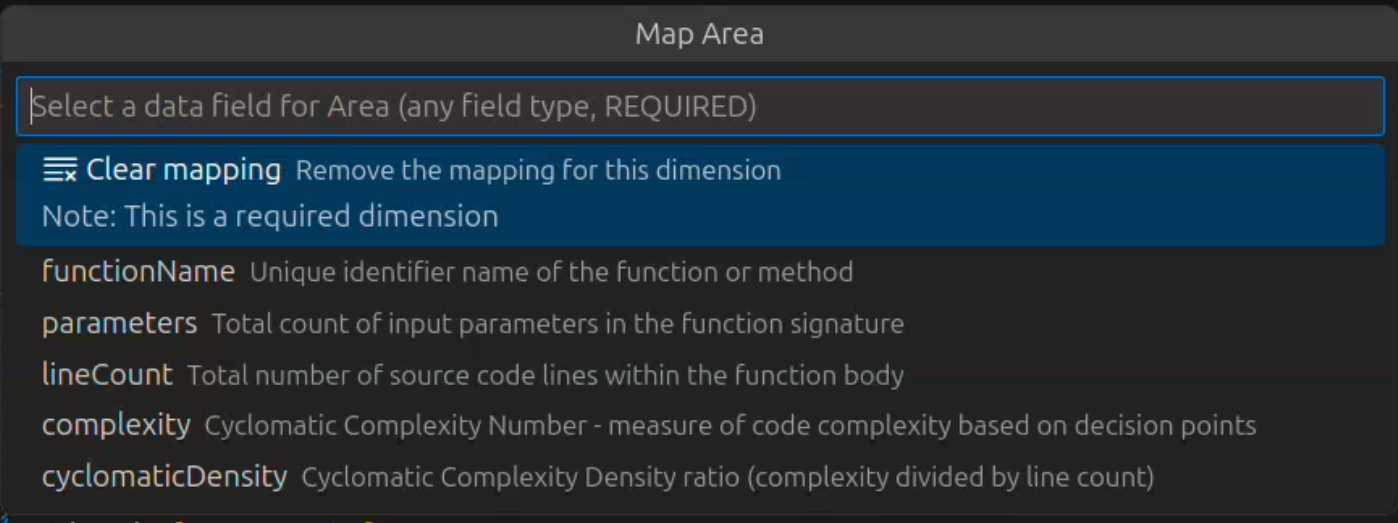
\includegraphics[width=\textwidth]{img/metricas-xr-ficheros.png}
\subcaption{Métricas disponibles para análisis XR de ficheros individuales}
\end{minipage}
\hfill
\begin{minipage}[b]{0.48\textwidth}
\centering
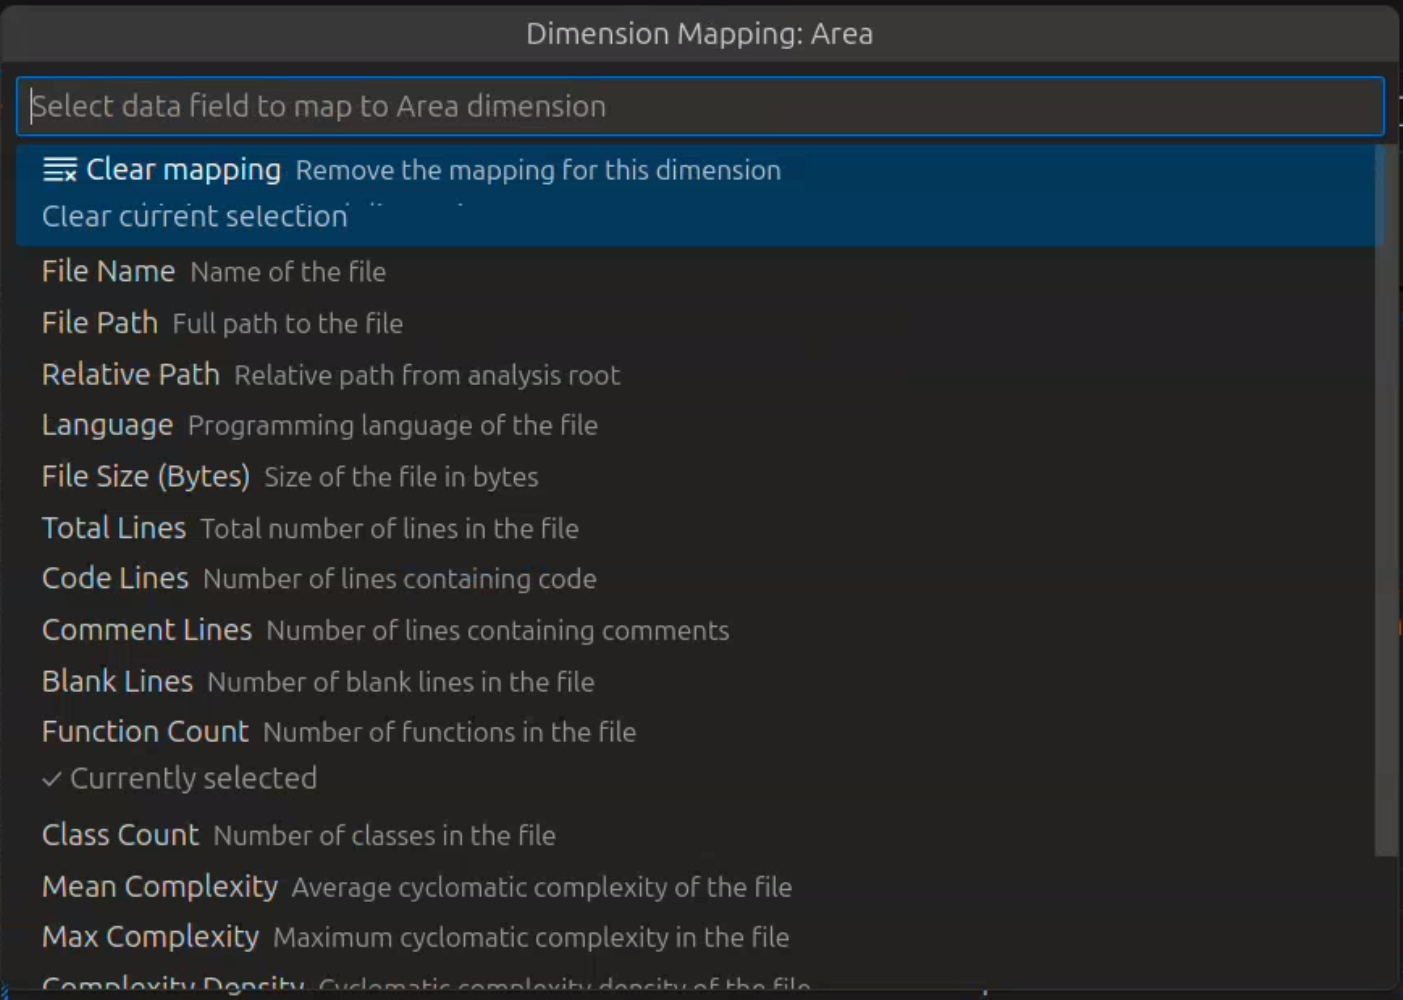
\includegraphics[width=\textwidth]{img/metricas-xr-directorios.png}
\subcaption{Métricas disponibles para análisis XR de directorios (muestra representativa)}
\end{minipage}
\caption{Interfaces de selección de métricas específicas en modo XR, mostrando las diferentes opciones disponibles según el alcance del análisis (fichero vs. directorio). La imagen de directorios muestra una buena muestra del total de métricas disponibles, aunque no se visualizan todas debido a limitaciones de espacio en la interfaz.}
\label{fig:metricas-xr-disponibles}
\end{figure}

\paragraph{Optimización y análisis incremental}
Estrategias de optimización para rendimiento ágil:

\begin{itemize}
  \item \textbf{Análisis incremental}: Re-analiza solo archivos modificados
  \item \textbf{Paralelización}: Distribuye análisis entre múltiples procesos Python
  \item \textbf{Caching}: Almacena resultados intermedios para acelerar análisis futuros
  \item \textbf{Análisis progresivo}: Retorna métricas esenciales rápidamente, completa detalles en segundo plano
\end{itemize}

\subsection{Gestión de sesiones de análisis}
\label{sec:gestion-sesiones}

La gestión de sesiones constituye el mecanismo central para coordinar análisis simultáneos, persistir configuraciones y gestionar el ciclo de vida completo de cada análisis, fundamental para la naturaleza en tiempo real de Code-XR.

\paragraph{Registro centralizado de sesiones}
El sistema implementa el patrón Registry a través de \texttt{UnifiedSessionRegistry}, proporcionando:

\begin{itemize}
  \item Repositorio centralizado con identificadores únicos (UUID v4)
  \item Control de transiciones de estado (creada → analizando → monitorizando/error)
  \item Gestión de metadatos, progreso y recursos asociados
  \item Prevención de duplicación de análisis idénticos
  \item APIs para consultas por ID, ruta o estado
\end{itemize}

\paragraph{Modelo de estado de sesión}
Ciclo de vida con estados discretos y transiciones estrictas:

\begin{enumerate}
  \item \textbf{created}: Sesión inicializada, análisis pendiente
  \item \textbf{analyzing}: Análisis en progreso con porcentaje opcional
  \item \textbf{monitoring}: Análisis completado, observando cambios
  \item \textbf{error}: Error que impide continuar
  \item \textbf{closed}: Sesión terminada, recursos liberándose
\end{enumerate}

% TODO: Añadir diagrama de estados de la sesión de análisis, mostrando las transiciones válidas
% Nombre sugerido: img/sesion-analisis-estados.png

\paragraph{Estructura de una sesión de análisis}
Cada sesión \texttt{UnifiedAnalysisSession} captura información completa para gestión autónoma: identificación (ID, ruta, tipo), estado y progreso, recursos asociados (hash, directorio, watcher, puerto, URL) y configuración (archivos requeridos, archivos a monitorizar).

\paragraph{Persistencia de configuraciones y resultados}
Esquema sofisticado de persistencia multinivel:

\begin{itemize}
  \item \textbf{Archivos de análisis}: Directorio único por sesión en \texttt{workspaceStorage} con HTML/CSS/JS, \texttt{data.json}, metadatos y recursos auxiliares
  \item \textbf{Persistencia temporal}: Archivos mantenidos durante sesión VS Code para reanudación rápida
  \item \textbf{Configuraciones personalizadas}: Almacenadas en \texttt{globalState} para reutilización
\end{itemize}

% TODO: Añadir diagrama de la estructura de almacenamiento en workspaceStorage para una sesión
% Nombre sugerido: img/sesion-almacenamiento-estructura.png

\paragraph{Gestión del ciclo de vida y liberación de recursos}
Control de recursos para prevenir fugas de memoria y bloqueos de puertos:

\begin{itemize}
  \item \textbf{Registro de recursos}: Referencias explícitas a watchers, servidores y archivos temporales
  \item \textbf{Liberación coordinada}: Detención ordenada de watchers, cierre de servidores HTTP/SSE, liberación de puertos y marcado de archivos para eliminación
  \item \textbf{Limpieza automática}: Al desactivar extensión, limpieza periódica de sesiones inactivas y al cerrar VS Code
  \item \textbf{Recuperación ante fallos}: Detección de puertos abandonados, watchers huérfanos y regeneración de archivos corruptos
\end{itemize}

\paragraph{Arquitectura de eventos y notificaciones}
\texttt{SessionRegistry} implementa sistema de eventos para arquitectura desacoplada:

\begin{itemize}
  \item \textbf{Eventos de ciclo de vida}: Notifican creación, cambio de estado y cierre
  \item \textbf{Eventos de progreso}: Indican avances en análisis
  \item \textbf{Eventos de error}: Comunican problemas durante análisis
\end{itemize}

\paragraph{Integración con watchers y servidores}
Coordinación con subsistemas asociados: cada sesión mantiene watchers específicos, servidores activos con canales SSE, asignación de puertos únicos y configuración de debounce a nivel sesión, garantizando operación autónoma sin interferencias entre sesiones.

\subsection{Tipos de análisis}
\label{sec:tipos-analisis}

El subsistema de análisis de Code-XR ofrece tres tipos de análisis distintos, cada uno especializado en extraer diferentes aspectos del código fuente. Estos tipos de análisis determinan qué métricas se calculan y cómo se estructuran los datos, pudiendo visualizarse posteriormente en panel lateral, navegador web o dispositivos VR/AR según la configuración del servidor.

\paragraph{LivePanel: análisis tradicional de métricas de código}
El análisis LivePanel extrae métricas completas de código fuente proporcionando información estructurada sobre complejidad, calidad y organización del código:

\begin{itemize}
  \item \textbf{Métricas de complejidad}: Complejidad ciclomática (CCN), densidad, profundidad de anidamiento y funciones críticas
  \item \textbf{Métricas estructurales}: Líneas de código, comentarios, clases, funciones y documentación
  \item \textbf{Análisis de calidad}: Ratios comentarios/código, funciones de alta complejidad y evaluación de documentación
  \item \textbf{Datos agregados}: Resúmenes por archivo, directorio y proyecto con estadísticas comparativas
\end{itemize}

% TODO: Añadir capturas del análisis LivePanel
% Nombre sugerido: img/livepanel-directorio-analisis.png y img/livepanel-fichero-analisis.png
\begin{figure}[H]
\centering
\begin{minipage}[b]{0.48\textwidth}
\centering
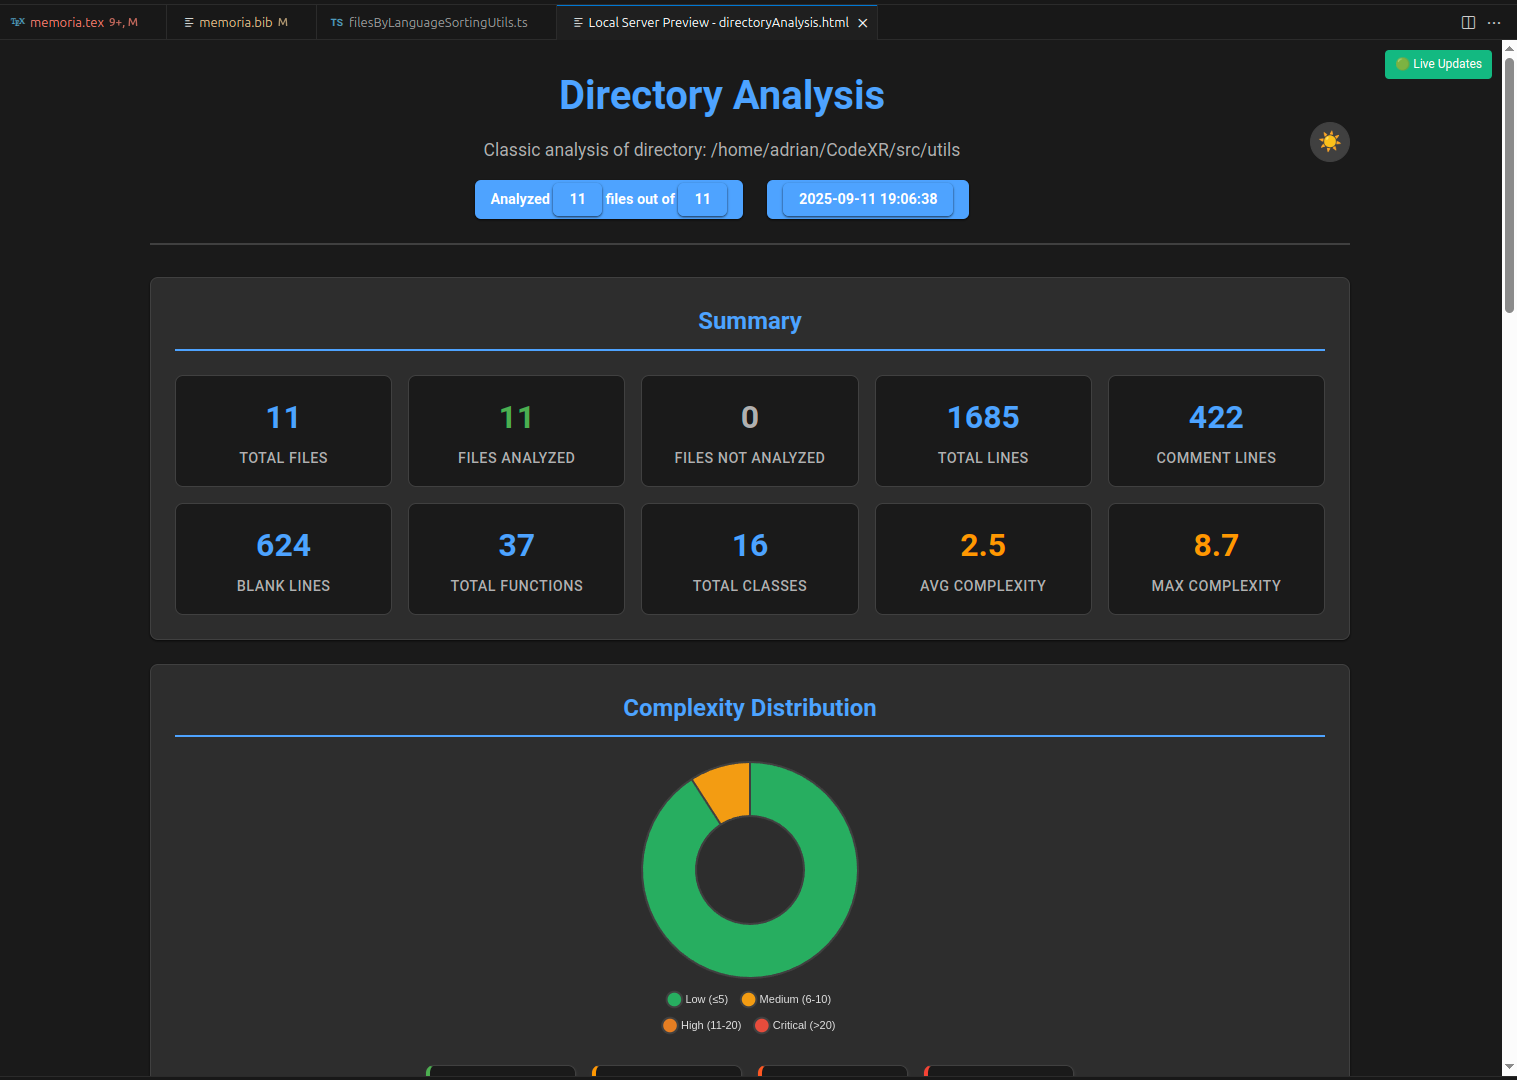
\includegraphics[width=\textwidth]{img/livepanel-directorio-analisis.png}
\subcaption{Análisis LivePanel de directorio}
\end{minipage}
\hfill
\begin{minipage}[b]{0.48\textwidth}
\centering
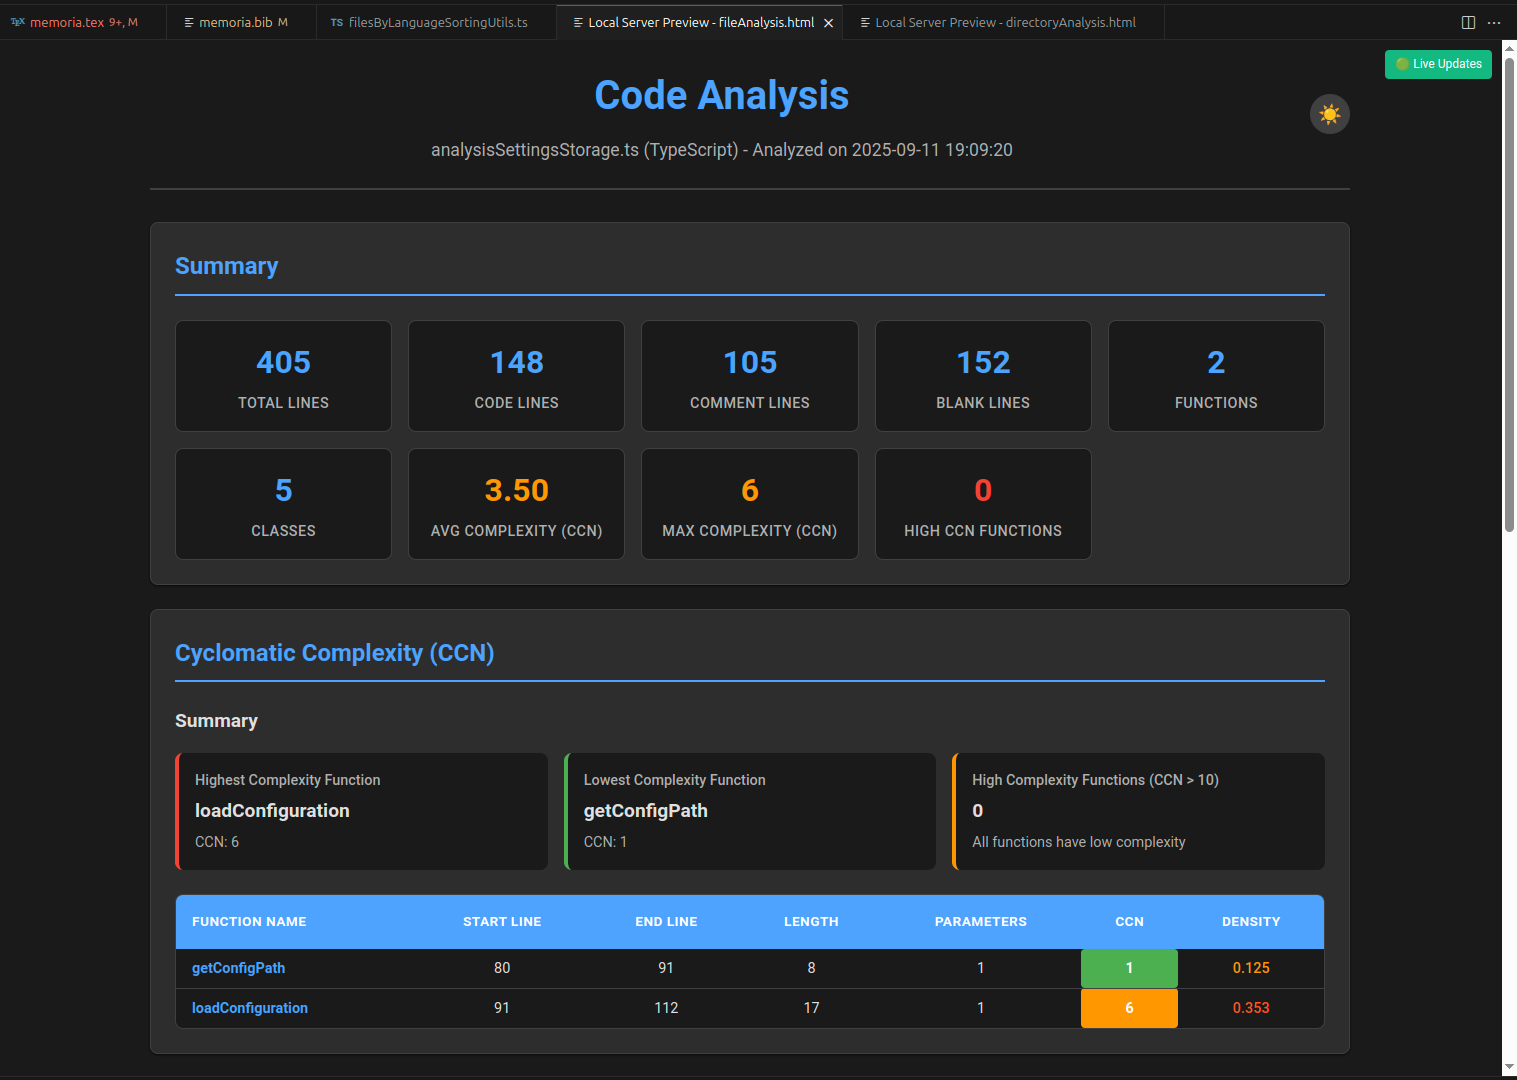
\includegraphics[width=\textwidth]{img/livepanel-fichero-analisis.png}
\subcaption{Análisis LivePanel de fichero individual}
\end{minipage}
\caption{Análisis LivePanel mostrando métricas tradicionales de código tanto para directorios completos como para ficheros individuales.}
\label{fig:livepanel-analisis}
\end{figure}

\paragraph{XR: análisis optimizado para visualización tridimensional}
El análisis XR procesa código fuente para generar representaciones espaciales tridimensionales, transformando métricas abstractas en elementos visuales navegables mediante A-Frame y BabiaXR:

\begin{itemize}
  \item \textbf{Transformación espacial}: Convierte métricas numéricas (complejidad, líneas) en propiedades visuales (altura, tamaño, color)
  \item \textbf{Mapeo de dimensiones}: Interface de selección específica que permite al usuario elegir qué métricas representar y cómo mapearlas a propiedades 3D
  \item \textbf{Agrupaciones inteligentes}: Organiza elementos por estructura del proyecto, tipos de archivo o métricas similares
  \item \textbf{Escalabilidad adaptativa}: Ajusta nivel de detalle según alcance (archivo individual, directorio, proyecto completo)
\end{itemize}

% TODO: Añadir capturas del análisis XR
% Nombre sugerido: img/xr-directorio-analisis.png, img/xr-fichero-analisis.png, img/xr-experiencia-ar.png
\begin{figure}[H]
\centering
\begin{minipage}[b]{0.32\textwidth}
\centering
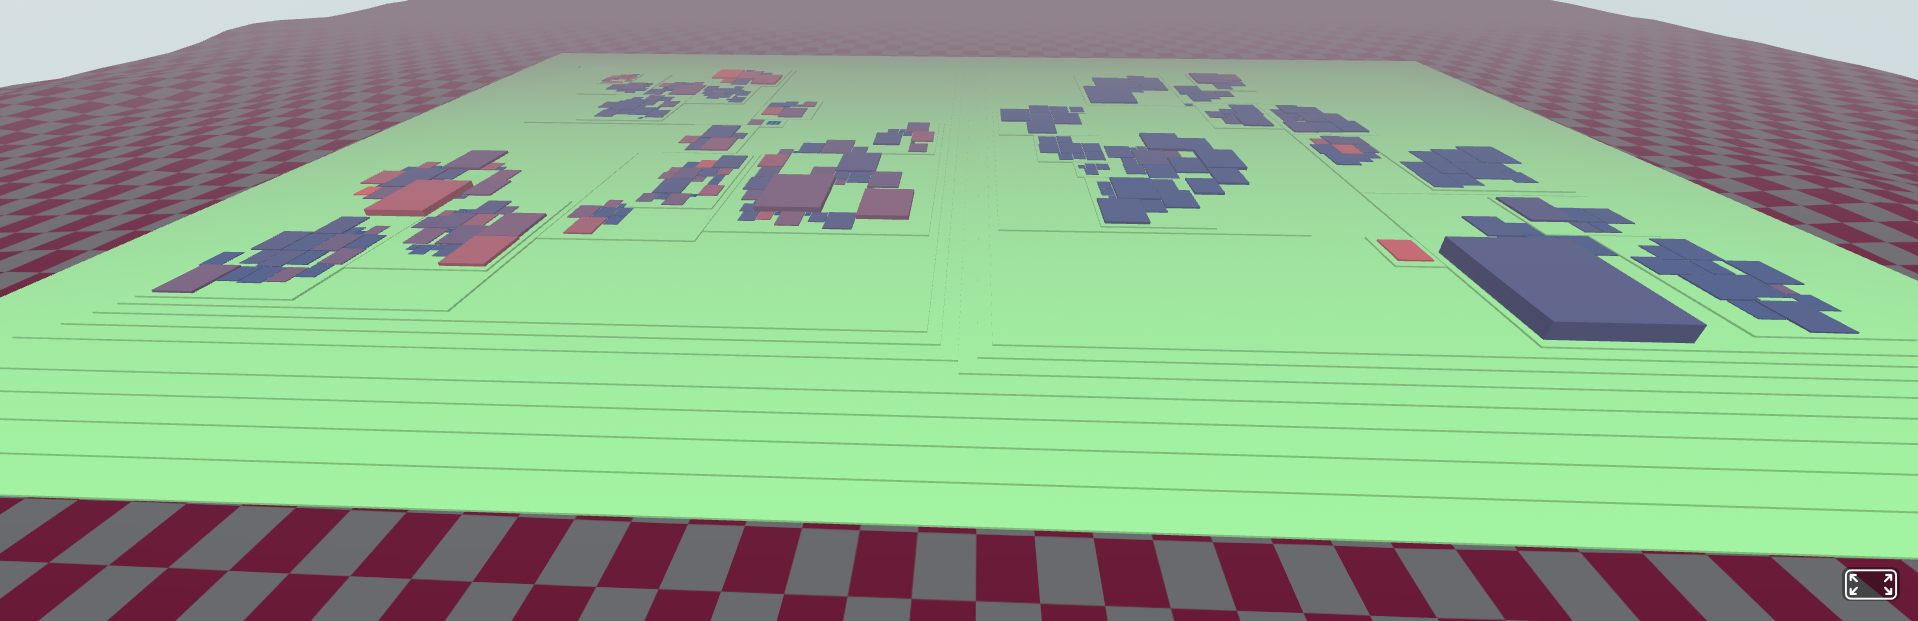
\includegraphics[width=\textwidth]{img/analisis-proyecto-completo.png}
\subcaption{Análisis XR de directorio}
\end{minipage}
\hfill
\begin{minipage}[b]{0.32\textwidth}
\centering
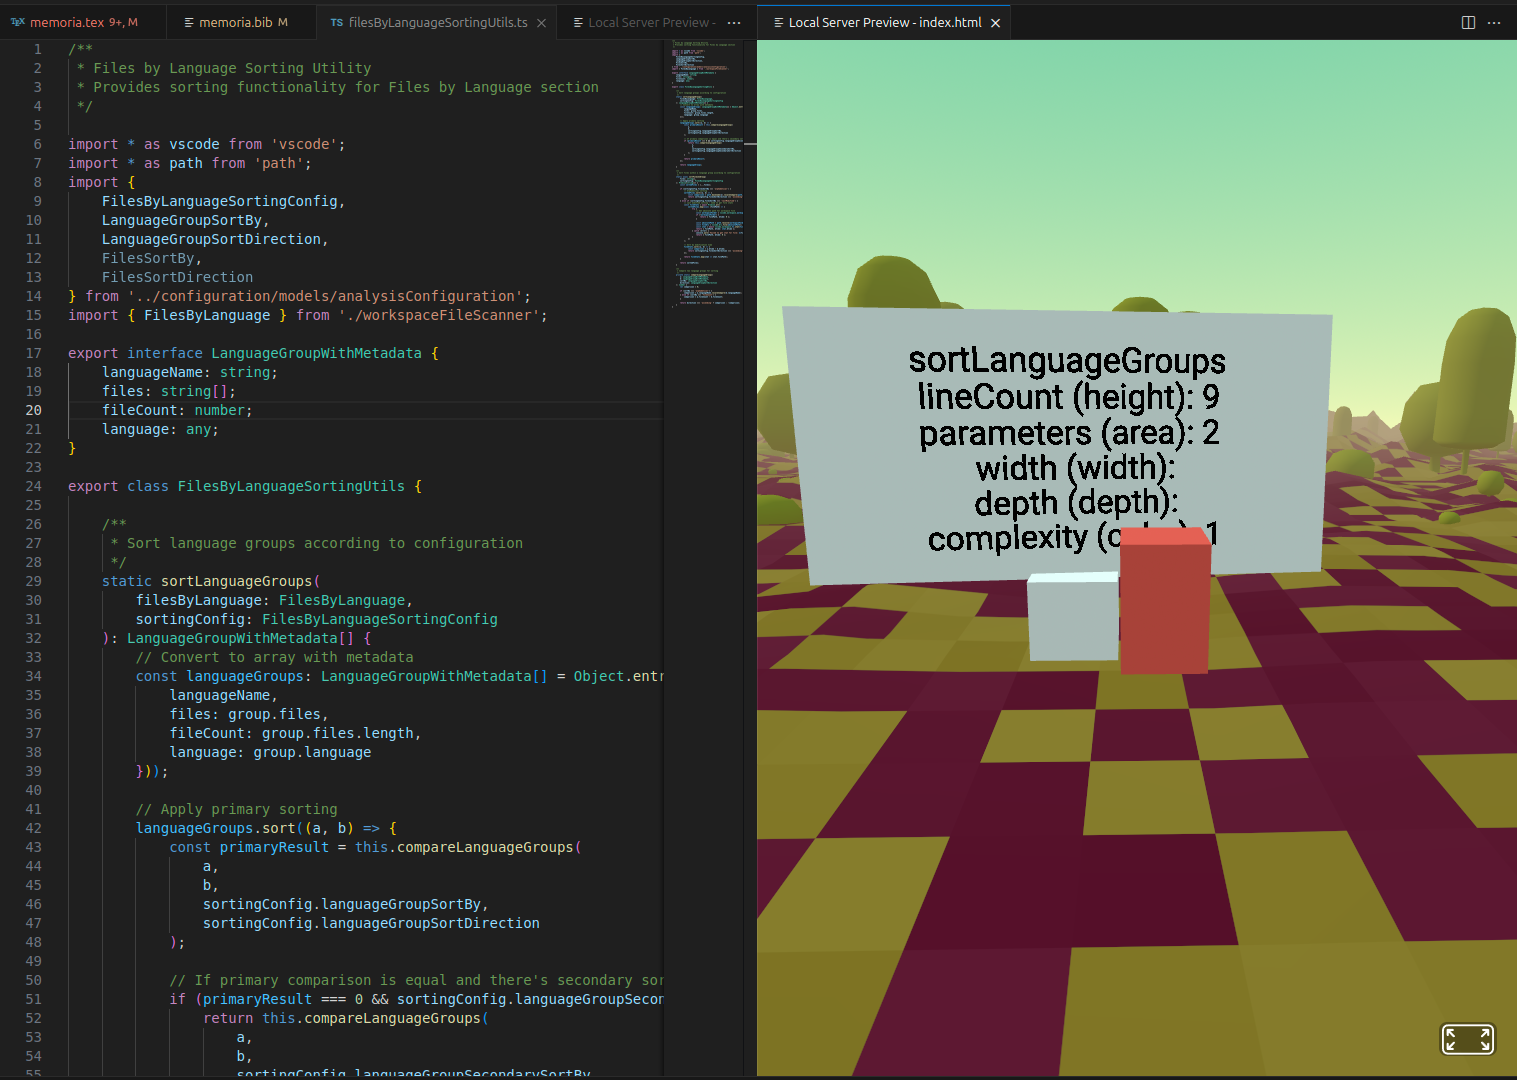
\includegraphics[width=\textwidth]{img/xr-fichero-analisis.png}
\subcaption{Análisis XR de fichero}
\end{minipage}
\hfill
\begin{minipage}[b]{0.32\textwidth}
\centering
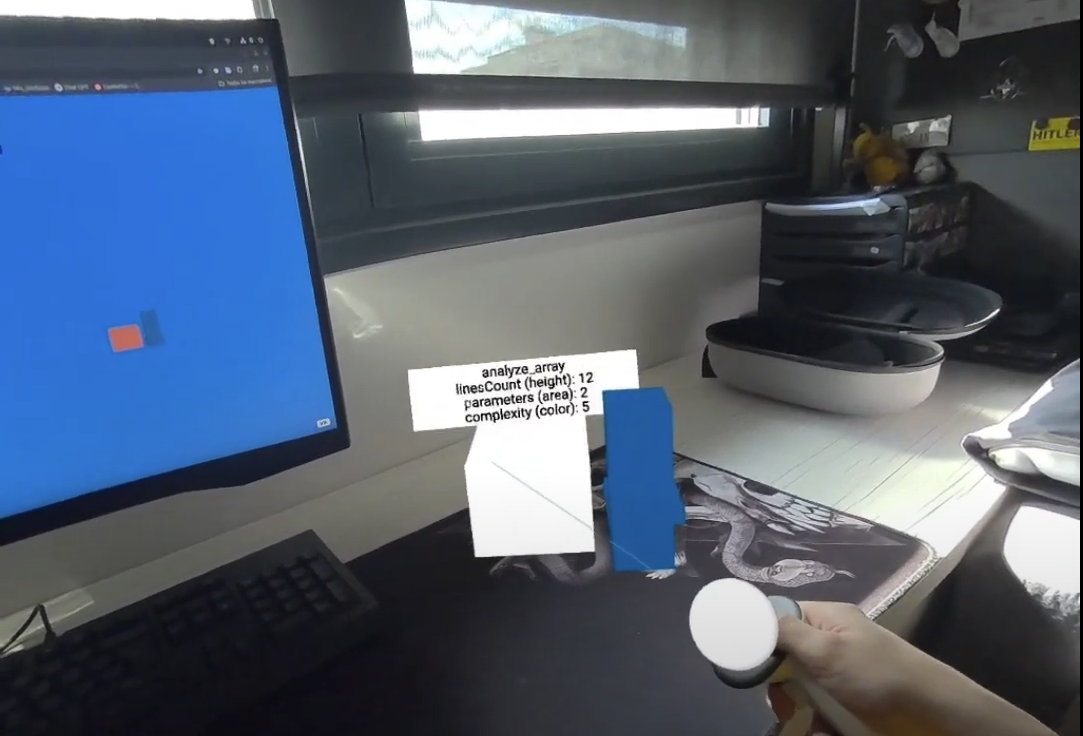
\includegraphics[width=\textwidth]{img/xr-experiencia-ar.png}
\subcaption{Experiencia AR/VR}
\end{minipage}
\caption{Análisis XR mostrando visualizaciones tridimensionales para diferentes alcances y su experiencia inmersiva en realidad aumentada.}
\label{fig:xr-analisis}
\end{figure}

\paragraph{DOM: análisis especializado para documentos HTML}
El análisis DOM está específicamente diseñado para extraer y procesar la estructura jerárquica de archivos HTML, transformando el Document Object Model en datos navegables para visualización tridimensional:

\begin{itemize}
  \item \textbf{Parsing de estructura DOM}: Analiza elementos HTML, atributos, anidamiento y relaciones padre-hijo
  \item \textbf{Detección de patrones}: Identifica estructuras problemáticas, anidamiento excesivo y elementos huérfanos
  \item \textbf{Representación jerárquica}: Genera datos optimizados para representación como árbol tridimensional navegable
\end{itemize}

% TODO: Añadir capturas del análisis DOM
% Nombre sugerido: img/dom-analisis-html.png, img/dom-experiencia-ar.png
\begin{figure}[H]
\centering
\begin{minipage}[b]{0.48\textwidth}
\centering
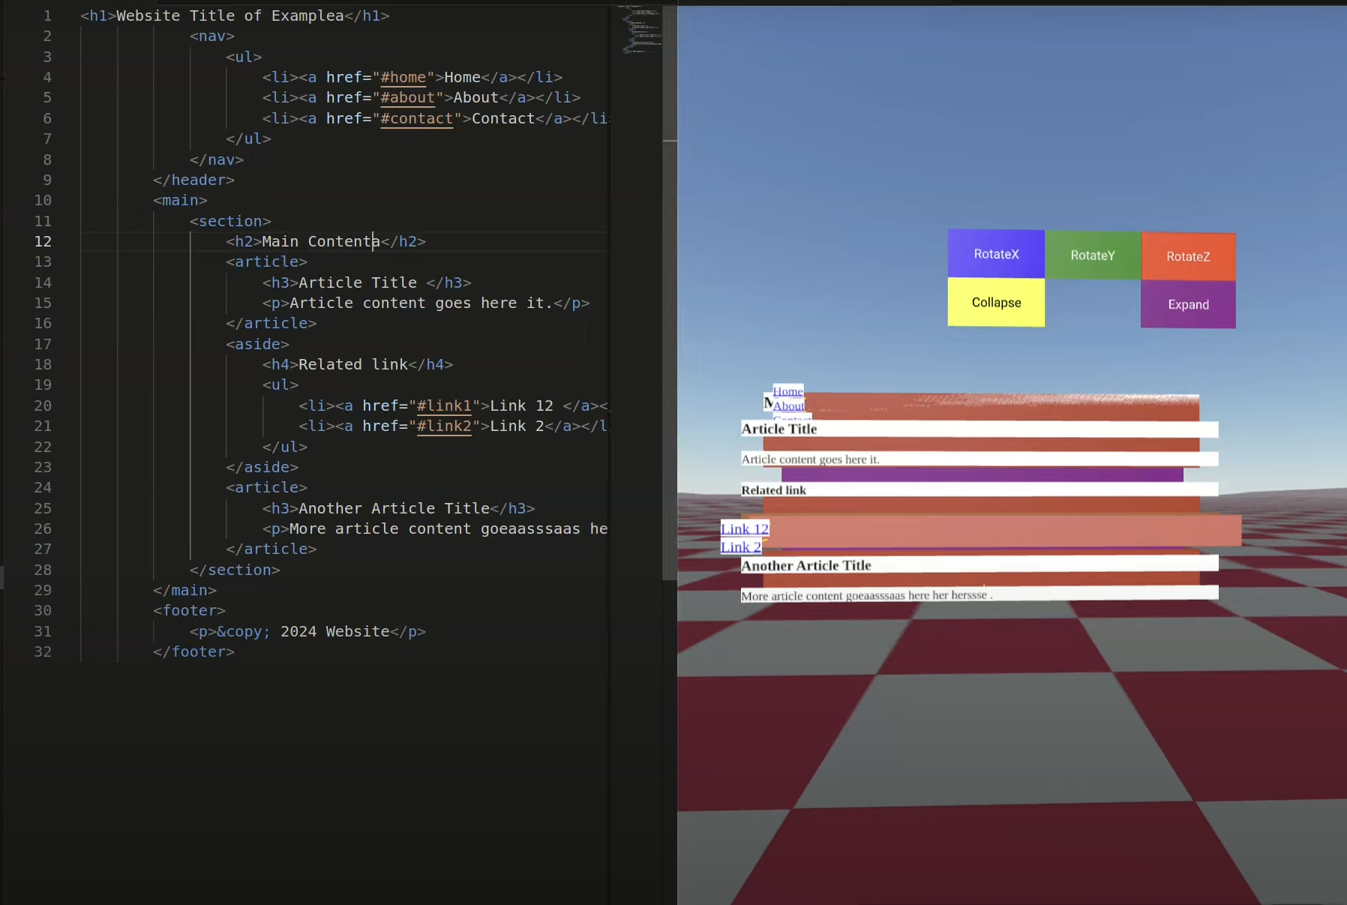
\includegraphics[width=\textwidth]{img/dom-analisis-html.png}
\subcaption{Análisis DOM de documento HTML}
\end{minipage}
\hfill
\begin{minipage}[b]{0.48\textwidth}
\centering
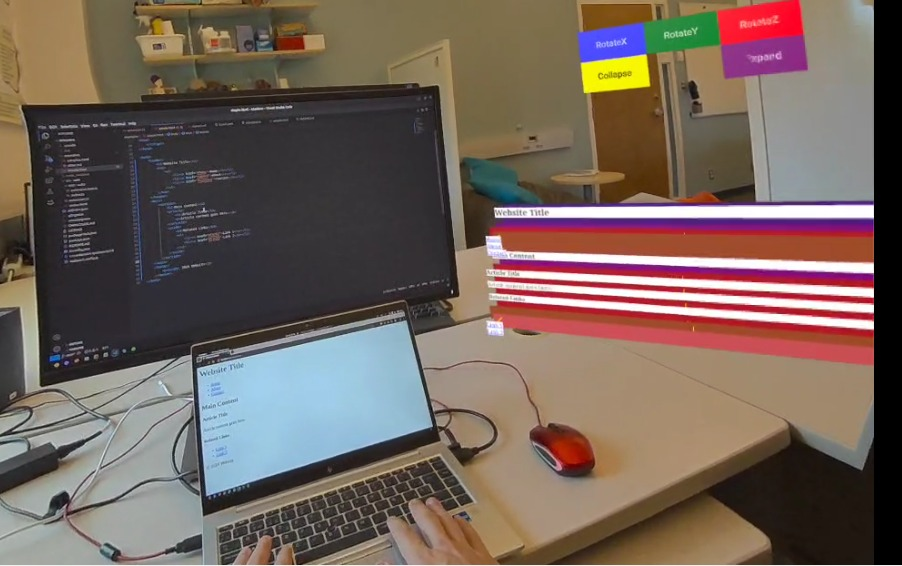
\includegraphics[width=\textwidth]{img/dom-experiencia-ar.png}
\subcaption{Experiencia AR del árbol DOM}
\end{minipage}
\caption{Análisis DOM mostrando la estructura jerárquica de documentos HTML y su representación inmersiva en realidad aumentada.}
\label{fig:dom-analisis}
\end{figure}

\paragraph{Modos de visualización universales}
Independientemente del tipo de análisis seleccionado (LivePanel, XR o DOM), todos pueden visualizarse según la configuración de lanzamiento del servidor establecida en el Sprint~\ref{sec:sprint-servers}:

\begin{itemize}
  \item \textbf{Panel lateral integrado}: Visualización directa dentro de VS Code mediante WebViews, manteniendo el contexto de desarrollo
  \item \textbf{Navegador web}: Apertura en navegador externo para visualización de pantalla completa con mejor rendimiento
  \item \textbf{Dispositivos VR/AR}: Acceso desde dispositivos de realidad virtual o aumentada conectados a la misma red
\end{itemize}


\subsection{Análisis en tiempo real}
\label{sec:analisis-tiempo-real}

Code-XR proporciona análisis en tiempo real mediante actualización automática de visualizaciones durante la edición de código, ofreciendo retroalimentación inmediata sobre calidad y estructura del software.

\paragraph{Sistema de watchers para detección de cambios}
Sistema sofisticado de observadores de archivos mediante \texttt{FileSystemWatcher} de VS Code:

\begin{itemize}
  \item \textbf{Watchers granulares}: Observadores específicos por archivo/directorio con creación/destrucción dinámica
  \item \textbf{Gestión por sesión}: Cada sesión mantiene watchers independientes para análisis paralelos
  \item \textbf{Filtros inteligentes}: Exclusión automática de archivos irrelevantes (configuración, binarios)
  \item \textbf{Eventos detectados}: \texttt{create}, \texttt{change}, \texttt{delete}, \texttt{rename}
\end{itemize}

\paragraph{Estrategia de debounce para optimización}
Agrupación de eventos cercanos temporalmente para evitar análisis excesivos:

\begin{itemize}
  \item \textbf{Temporizador configurable}: Intervalo ajustable (predeterminado: 1000ms)
  \item \textbf{Agrupación inteligente}: Múltiples cambios procesados como evento único
  \item \textbf{Reconfiguración dinámica}: Actualización sin reinicio de análisis
\end{itemize}

\paragraph{Análisis incremental y diferencial}
Optimización mediante procesamiento selectivo de modificaciones:

\begin{itemize}
  \item \textbf{Detección por hash}: Identificación de modificaciones reales mediante hash de contenido
\end{itemize}

\paragraph{Sincronización de cambios con visualizaciones}
Mecanismo robusto de propagación desde detección hasta actualización visual:

\begin{enumerate}
  \item \textbf{Detección}: Watcher identifica modificación
  \item \textbf{Debounce}: Espera intervalo sin cambios adicionales
  \item \textbf{Re-análisis}: Ejecución del motor Python solo en archivos modificados
  \item \textbf{Actualización datos}: Generación de nuevo \texttt{data.json}
  \item \textbf{Evento SSE}: Emisión de \texttt{analysis-updated}
  \item \textbf{Actualización cliente}: Solicitud y renderizado incremental
\end{enumerate}

\begin{figure}[H]
\centering
\begin{tikzpicture}[
  node distance=1.3cm and 2cm,
  event/.style={rectangle, draw, rounded corners, fill=blue!10, minimum width=3cm, minimum height=0.8cm, align=center},
  process/.style={rectangle, draw, fill=green!10, minimum width=3cm, minimum height=0.8cm, align=center},
  decision/.style={diamond, draw, fill=yellow!10, minimum width=2cm, minimum height=0.8cm, align=center, inner sep=0pt},
  flow/.style={thick,-latex}
]

% Nodes
\node[event] (change) {Cambio en archivo};
\node[process, right=of change] (debounce) {Aplicar debounce};
\node[decision, right=of debounce] (nochanges) {¿Más cambios?};
\node[process, below=of nochanges] (analyze) {Re-analizar archivo};
\node[process, below=of analyze] (update) {Actualizar data.json};
\node[process, below=of update] (emit) {Emitir evento SSE};
\node[process, left=of emit] (receive) {Cliente recibe evento};
\node[process, left=of receive] (request) {Solicitar datos};
\node[process, above=of request] (render) {Actualizar visualización};

% Connections
\draw[flow] (change) -- (debounce);
\draw[flow] (debounce) -- (nochanges);
\draw[flow] (nochanges) -- node[right] {No} (analyze);
\draw[flow] (nochanges) -- node[above] {Sí} ++(-1.5,0) -- ++(0,1.5) -- (debounce);
\draw[flow] (analyze) -- (update);
\draw[flow] (update) -- (emit);
\draw[flow] (emit) -- (receive);
\draw[flow] (receive) -- (request);
\draw[flow] (request) -- (render);
\draw[flow] (render) -- ++(-1.5,0) -- ++(0,3.0) -- (change);

\end{tikzpicture}
\caption{Diagrama del ciclo de re-análisis y actualización en tiempo real.}
\label{fig:reanalisis-ciclo}
\end{figure}

\paragraph{Rendimiento y optimización}
Optimizaciones para mantener capacidad de respuesta en proyectos grandes:

\begin{itemize}
  \item \textbf{Análisis por lotes}: Procesamiento de archivos en lotes para evitar bloqueo de UI
  \item \textbf{Procesamiento asíncrono}: Operaciones en hilos separados
  \item \textbf{Limitación adaptativa}: Restricciones dinámicas según carga del sistema
  \item \textbf{Cancelación inteligente}: Cancelación automática de análisis obsoletos
\end{itemize}

\subsection{Comunicación en tiempo real (SSE)}
\label{sec:comunicacion-sse}

Code-XR reutiliza la infraestructura de Server-Sent Events (SSE) desarrollada en el Sprint~\ref{sec:sprint-servers} para proporcionar actualizaciones asíncronas en tiempo real de las visualizaciones durante el análisis de código, eliminando la necesidad de recargar manualmente y ofreciendo retroalimentación inmediata.

\paragraph{Reutilización de la arquitectura SSE del Sprint 1}
Cada sesión de análisis aprovecha el sistema de servidores HTTP/HTTPS establecido previamente, manteniendo canales SSE dedicados para comunicar cambios entre el motor de análisis y las visualizaciones activas.

\paragraph{Flujo de comunicación entre backend y frontend}
Patrón secuencial optimizado que conecta análisis con visualización:

\begin{enumerate}
  \item \textbf{Conexión}: cliente conecta automáticamente a endpoint SSE
  \item \textbf{Estado inicial}: servidor envía estado actual inmediatamente
  \item \textbf{Eventos}: listeners configurados para cada tipo, actualización UI correspondiente
  \item \textbf{Datos}: evento \texttt{analysis-updated} → petición HTTP a \texttt{/data.json}
  \item \textbf{Actualización parcial}: solo componentes afectados, preservando navegación
  \item \textbf{Reconexión}: automática con backoff exponencial
\end{enumerate}

\begin{figure}[H]
\centering
\begin{tikzpicture}[
  node distance=2cm,
  system/.style={rectangle, draw, minimum width=3cm, minimum height=2cm, align=center},
  event/.style={rectangle, draw, rounded corners, fill=blue!10, minimum width=2.5cm, align=center},
  arrow/.style={thick,-latex},
  dasharrow/.style={thick,-latex,dashed}
]

% Systems
\node[system] (backend) {Backend \\ (Análisis)};
\node[system, right=5cm of backend] (frontend) {Frontend \\ (Visualización)};

% Timeline
\draw[thick] (backend.south) -- ++(0,-8);
\draw[thick] (frontend.south) -- ++(0,-8);

% Events
\coordinate[below=0.8cm of backend.south] (b1);
\coordinate[below=0.8cm of frontend.south] (f1);
\node[event, left=0.3cm of b1] (e1) {Re-análisis};

\coordinate[below=1.5cm of b1] (b2);
\coordinate[below=1.5cm of f1] (f2);
\node[event, right=0.3cm of f2] (e2) {Conexión SSE};

\coordinate[below=1.0cm of b2] (b3);
\coordinate[below=1.0cm of f2] (f3);
\node[event, left=0.3cm of b3] (e3) {Actualización data.json};

\coordinate[below=1.0cm of b3] (b4);
\coordinate[below=1.0cm of f3] (f4);
\node[event, left=0.3cm of b4] (e4) {Envío evento SSE};

\coordinate[below=1.0cm of b4] (b5);
\coordinate[below=1.0cm of f4] (f5);
\node[event, right=0.3cm of f5] (e5) {Recepción evento};

\coordinate[below=1.0cm of b5] (b6);
\coordinate[below=1.0cm of f5] (f6);
\node[event, right=0.3cm of f6] (e6) {Solicitud data.json};

\coordinate[below=1.0cm of b6] (b7);
\coordinate[below=1.0cm of f6] (f7);
\node[event, right=0.3cm of f7] (e7) {Actualización UI};

% Connections
\draw[arrow] (f2) -- (b2) node[midway, above] {GET /events};
\draw[dasharrow] (b2) -- (f2) node[midway, below] {200 OK};
\draw[arrow] (f6) -- (b6) node[midway, above] {GET /data.json};
\draw[dasharrow] (b6) -- (f6) node[midway, below] {200 OK + JSON};
\draw[dasharrow] (b4) -- (f5) node[midway, below] {analysis-updated};

% Event connections
\draw[arrow] (e1) -- (b1);
\draw[arrow] (e2) -- (f2);
\draw[arrow] (e3) -- (b3);
\draw[arrow] (e4) -- (b4);
\draw[arrow] (e5) -- (f5);
\draw[arrow] (e6) -- (f6);
\draw[arrow] (e7) -- (f7);

% Vertical connections
\draw[arrow] (b1) -- (b2);
\draw[arrow] (b2) -- (b3);
\draw[arrow] (b3) -- (b4);
\draw[arrow] (b4) -- (b5);
\draw[arrow] (b5) -- (b6);
\draw[arrow] (b6) -- (b7);
\draw[arrow] (f2) -- (f3);
\draw[arrow] (f3) -- (f4);
\draw[arrow] (f4) -- (f5);
\draw[arrow] (f5) -- (f6);
\draw[arrow] (f6) -- (f7);

\end{tikzpicture}
\caption{Diagrama del flujo de comunicación SSE entre el backend (análisis) y el frontend (visualización).}
\label{fig:sse-flujo}
\end{figure}

\paragraph{Implementación en diferentes modos de visualización}
Cada modo de visualización implementa el protocolo SSE de manera específica:

\begin{itemize}
  \item \textbf{LivePanel}: utiliza la API WebView de VS Code para cargar directamente el código JavaScript que establece la conexión SSE y actualiza el DOM según los eventos recibidos.
  
  \item \textbf{XR}: implementa la lógica de conexión SSE en el código de A-Frame/BabiaXR, actualizando entidades y componentes 3D en respuesta a los eventos.
  
  \item \textbf{DOM Mode}: establece una conexión SSE dedicada para monitorear cambios en la estructura DOM del archivo HTML analizado.
\end{itemize}

\subsection{Configuración y personalización}
\label{sec:configuracion}

Code-XR implementa un sistema integral de configuración mediante interfaz dedicada en el panel lateral, permitiendo personalización completa del comportamiento de análisis y apariencia visual según necesidades específicas del usuario.

\paragraph{Interfaz de configuración unificada}
Panel centralizado organizando todas las opciones de personalización:

\begin{itemize}
  \item \textbf{Selección de análisis}: fichero individual o directorio completo, visualizable en LivePanel o XR, con opción \texttt{deep} para directorios que activa análisis exhaustivo de dependencias y relaciones
  \item \textbf{Tema visual LivePanel}: modo claro/oscuro optimizado para diferentes condiciones de iluminación, afectando únicamente visualizaciones LivePanel para mantener legibilidad
  \item \textbf{Gráficos XR}: selección entre tipos BabiaXR especializados (Bar, Barsmap, Bubble, Cylinder, Boats) según Figura~\ref{fig:visualize-chart-selector}, cada uno optimizado para diferentes tipos de datos y densidades
  \item \textbf{Mapeo de dimensiones XR}: asignación flexible de campos de datos a propiedades visuales XR (key, size, color, height, area) con validación automática de tipos numéricos y compatibilidad de datos, referenciado en Figura~\ref{fig:metricas-xr-disponibles}
  \item \textbf{Parámetros de ejecución}: debounce time configurable para análisis consecutivos evitando sobrecarga durante edición continua, auto-análisis automático activable post-guardado para retroalimentación inmediata
  \item \textbf{Ordenación Files by Language}: criterios jerárquicos primario/secundario (alfabético/tamaño/fecha), dirección ascendente/descendente, orden interno personalizable por fecha de modificación o alfabético para organización óptima del workspace

\paragraph{Valores por defecto del sistema}
La configuración inicial incorpora valores optimizados basados en análisis de usabilidad y rendimiento:

\begin{itemize}
  \item \textbf{Fichero de análisis}: XR - análisis en fichero individual por defecto minimizando sobrecarga computacional
  \item \textbf{Directorio de análisis}: XR (sin deep) - análisis superficial preservando rendimiento, evitando análisis recursivo exhaustivo de dependencias
  \item \textbf{Tema visual}: Dark - optimizado para sesiones prolongadas de desarrollo, reduciendo fatiga visual en entornos de trabajo típicos de IDE
  \item \textbf{Tipo de gráfico}: Boats - visualización equilibrada entre densidad de información y navegabilidad XR para ambos contextos (ficheros y directorios)
  \item \textbf{Mapeo de dimensiones ficheros}: Area=parameters, Height=lineCount, Color=Complexity - correlación directa entre complejidad estructural y propiedades visuales XR
  \item \textbf{Mapeo de dimensiones directorios}: Area=Function Count, Height=total Lines, Color=Mean Complexity - métricas agregadas representando características arquitecturales del módulo
  \item \textbf{Debounce time}: 3 segundos - equilibrio entre responsividad y eficiencia computacional durante edición activa de código
  \item \textbf{Auto-análisis}: Habilitado - retroalimentación automática post-guardado facilitando desarrollo iterativo y detección temprana de issues
  \item \textbf{Ordenación Files by Language}: Primaria alfabética ascendente, secundaria desactivada - organización intuitiva del workspace por nomenclatura estándar de ficheros
  \item \textbf{Ordenación Files}: alfabética ascendente - consistencia en presentación de resultados independiente del contexto de análisis
\end{itemize}
\end{itemize}

% TODO: Añadir captura completa del panel de configuración mostrando todas las opciones descritas
% Nombre sugerido: img/panel-configuracion-completo.png
\begin{figure}[H]
\centering
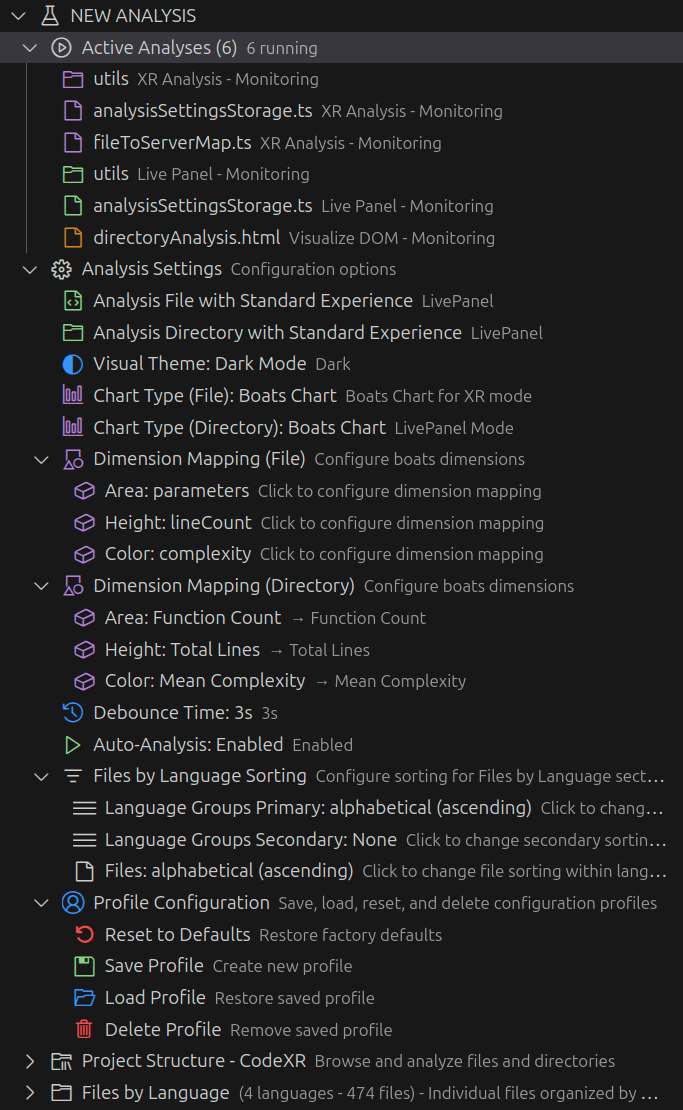
\includegraphics[width=0.9\textwidth]{img/panel-configuracion-completo.png}
\caption{Panel de configuración completo de Code-XR mostrando todas las opciones de personalización: selección de análisis, tema visual, gráficos XR, mapeo de dimensiones, parámetros de ejecución y ordenación.}
\label{fig:panel-configuracion-completo}
\end{figure}

\paragraph{Integración con Visualization Settings}
Herencia completa de configuraciones estéticas del Sprint 2: Background Color (fondo visualizaciones), Ground Color (suelo XR), Environment Preset (ambientes virtuales forest/tron/dream), Chart Palette (esquemas cromáticos). Garantiza coherencia visual entre ejemplos BabiaXR, visualizaciones JSON y análisis de código.

\paragraph{Interfaz de configuración}
Code-XR proporciona múltiples puntos de acceso para gestionar la configuración:

\begin{itemize}
  \item \textbf{Panel de configuración de VS Code}: integrado con la configuración estándar del editor bajo la sección \texttt{codeXR}.
  
  \item \textbf{Comandos rápidos}: accesibles mediante la paleta de comandos (F1) para cambios comunes.
  
  \item \textbf{Menú contextual}: opciones específicas disponibles con clic derecho en archivos y carpetas.
  
  \item \textbf{Árbol de extensión}: opciones accesibles desde los nodos del árbol de Code-XR en el panel lateral.
  
  \item \textbf{Configuración por sesión}: opciones disponibles en la propia interfaz de visualización para ajustes específicos.
\end{itemize}

% TODO: Añadir captura de pantalla del panel de configuración de análisis
% Nombre sugerido: img/panel-configuracion-analisis.png

\paragraph{Gestión de perfiles de usuario}
Sistema de perfiles para persistencia y reutilización de configuraciones personalizadas:

\begin{itemize}
  \item \textbf{Operaciones básicas}: guardar, cargar, resetear y eliminar perfiles de configuración
  \item \textbf{Reutilización}: aplicación de ajustes específicos en diferentes sesiones de trabajo
  \item \textbf{Persistencia}: almacenamiento en \texttt{globalState} para disponibilidad entre sesiones VS Code
\end{itemize}

\paragraph{Gestión de análisis activos}
Sección \texttt{Active Analyses} para monitoreo y control de sesiones en ejecución:

\begin{itemize}
  \item \textbf{Acceso rápido}: lista completa de análisis lanzados con información de estado
  \item \textbf{Menú contextual}: opciones específicas mediante clic derecho
  \begin{itemize}
    \item \texttt{View Details}: visualización completa de metadatos de sesión (Session ID, ruta objetivo, modo, timestamps, configuración, progreso)
    \item \texttt{Open in Browser}: apertura directa del servidor de análisis en navegador externo
    \item \texttt{Stop Analysis}: detención del análisis manteniendo servidor activo para visualización del estado final
  \end{itemize}
  \item \textbf{Coordinación con Active Servers}: cierre de servidor desde Active Servers detiene análisis correspondiente automáticamente
\end{itemize}

Estructura de perfil encapsulando configuración completa:

\begin{figure}[H]
\centering
\begin{lstlisting}[
language=JSON,
basicstyle=\tiny\ttfamily,
frame=single,
breaklines=true,
keywordstyle=\color{red},
stringstyle=\color{blue},
numberstyle=\color{green},
commentstyle=\color{gray},
xleftmargin=0.05cm,
xrightmargin=0.05cm,
showstringspaces=false]
{
  "metadata": {
    "version": "1.0.0",
    "createdBy": "CodeXR New Code Analysis"
  },
  "configuration": {
    "analysisFileMode": "XR",
    "analysisDirectoryMode": "XR",
    "viewTheme": "Dark",
    "autoAnalysisDelay": {
      "type": "3s",
      "autoAnalysisEnabled": true
    },
    "chartTypeFile": "boats",
    "chartTypeDirectory": "boats",
    "dimensionMappingFile": {
      "area": "parameters",
      "height": "lineCount",
      "color": "complexity"
    },
    "dimensionMappingDirectory": {
      "area": "functionCount",
      "height": "totalLines",
      "color": "cyclomaticComplexityNumber"
    },
    "filesByLanguageSorting": {
      "languageGroupSortBy": "alphabetical",
      "languageGroupSortDirection": "ascending",
      "filesSortBy": "alphabetical",
      "filesSortDirection": "ascending"
    }
  }
}
\end{lstlisting}
\caption{Estructura de un perfil de análisis en Code-XR mostrando el perfil por defecto con todas las configuraciones del sistema.}
\label{fig:profile-structure}
\end{figure}

\paragraph{Navegación de proyectos integrada}
Interfaces especializadas para lanzamiento directo de análisis:

\begin{itemize}
  \item \textbf{Project Structure}: árbol jerárquico de carpetas y archivos con análisis contextual directo
  \item \textbf{Files by Language}: agrupación automática por lenguaje detectado con análisis de fichero individual
\end{itemize}

\subsection{Optimización y extensibilidad}
\label{sec:optimizacion-extensibilidad}

El subsistema de análisis de Code-XR está diseñado con un enfoque en la optimización del rendimiento y la extensibilidad, permitiendo tanto un funcionamiento eficiente como la adición futura de nuevos tipos de análisis y visualizaciones.

\paragraph{Estrategias de optimización de rendimiento}
Optimizaciones para mantener rendimiento ágil en proyectos complejos:

\begin{itemize}
  \item \textbf{Análisis incremental}: Re-análisis exclusivo de archivos modificados preservando resultados previos
  \item \textbf{Paralelización}: Distribución entre múltiples procesos Python aprovechando núcleos disponibles
  \item \textbf{Procesamiento por lotes}: Archivos procesados en lotes configurables optimizando memoria y permitiendo visualizaciones parciales tempranas
  \item \textbf{Caché multinivel}: Memoria para resultados recientes, disco para persistencia entre sesiones, invalidación inteligente por hash de contenido
\end{itemize}

\paragraph{Arquitectura modular extensible}
Sistema de plugins facilitando adición de componentes sin modificar núcleo:

\begin{itemize}
  \item \textbf{Analizadores pluggable}: Interfaz común \texttt{CodeAnalyzer} con métodos \texttt{analyze()}, \texttt{canAnalyze()}, \texttt{supportedLanguages}
  \item \textbf{Visualizaciones extensibles}: Sistema templates y adaptadores mediante \texttt{VisualizationProvider} con \texttt{getTemplateFiles()}, \texttt{transformData()}
  \item \textbf{Motor plantillas}: Archivos HTML/CSS/JS con marcadores, sistema transformación, motor sustitución y biblioteca componentes reutilizables
\end{itemize}

\section{Nota sobre la documentación técnica del proyecto}
\label{sec:nota-documentacion}

La documentación técnica presentada a lo largo de este documento (Primeros pasos, Sprint 1, Sprint 2 y Sprint 3) constituye una síntesis significativa de la implementación completa de Code-XR. Debido a las limitaciones de espacio inherentes a una memoria de TFG, se ha condensado considerablemente la información técnica para destacar únicamente los aspectos arquitectónicos y funcionales más relevantes del sistema.

Para una comprensión completa y exhaustiva de todos los aspectos técnicos de la implementación, se recomienda encarecidamente consultar el repositorio público del proyecto: \url{https://github.com/aMonteSl/CodeXR}\cite{code-xr}

Todo el código fuente está disponible bajo licencia MIT, incluyendo documentación técnica completa, guías de desarrollo, ejemplos prácticos y recursos para facilitar la comprensión, extensión y contribución al proyecto por parte de desarrolladores e investigadores interesados.



%
%%%%%%%%%%%%%%%%%%%%%%%%%%%%%%%%%%%%%%%%%%%%%%%%%%%%%%%%%%%%%%%%%%%%%%%%%%%%%%%%
%%%%%%%%%%%%%%%%%%%%%%%%%%%%%%%%%%%%%%%%%%%%%%%%%%%%%%%%%%%%%%%%%%%%%%%%%%%%%%%%
% EXPERIMENTOS Y VALIDACIÓN %
%%%%%%%%%%%%%%%%%%%%%%%%%%%%%%%%%%%%%%%%%%%%%%%%%%%%%%%%%%%%%%%%%%%%%%%%%%%%%%%%

\cleardoublepage
\chapter{Experimentos y validación}
\label{chap:experimentos}

El objetivo fundamental de este TFG era la extracción y posteriormente la representación visual de métricas en experiencias XR gracias a A-Frame y BabiaXR. Además, el plugin ofrece la posibilidad de ver esas métricas en un formato más clásico gracias al análisis tipo LivePanel, y también permite visualizar el árbol DOM de un HTML en experiencia XR.

\section{Metodología de pruebas y depuración}
\label{sec:metodologia-pruebas}

Para verificar el correcto funcionamiento de todos los componentes del plugin, se implementó una estrategia de depuración completa:

\begin{itemize}
  \item \textbf{Depuración interna}: El plugin incluye numerosas trazas con \texttt{console.log}. Para depurarlo, lanzar el debugger con F5 en VS Code y abrir las \emph{Developer Tools} (Ctrl+Shift+I): allí se visualizan todos los logs y se puede seguir el flujo interno del plugin sin depender solo de su comportamiento visual.
\end{itemize}
% TODO: Añadir imagen de las Developer Tools con los console.logs del plugin
% Nombre sugerido: img/developer-tools-logs.png

\begin{figure}[H]
\centering
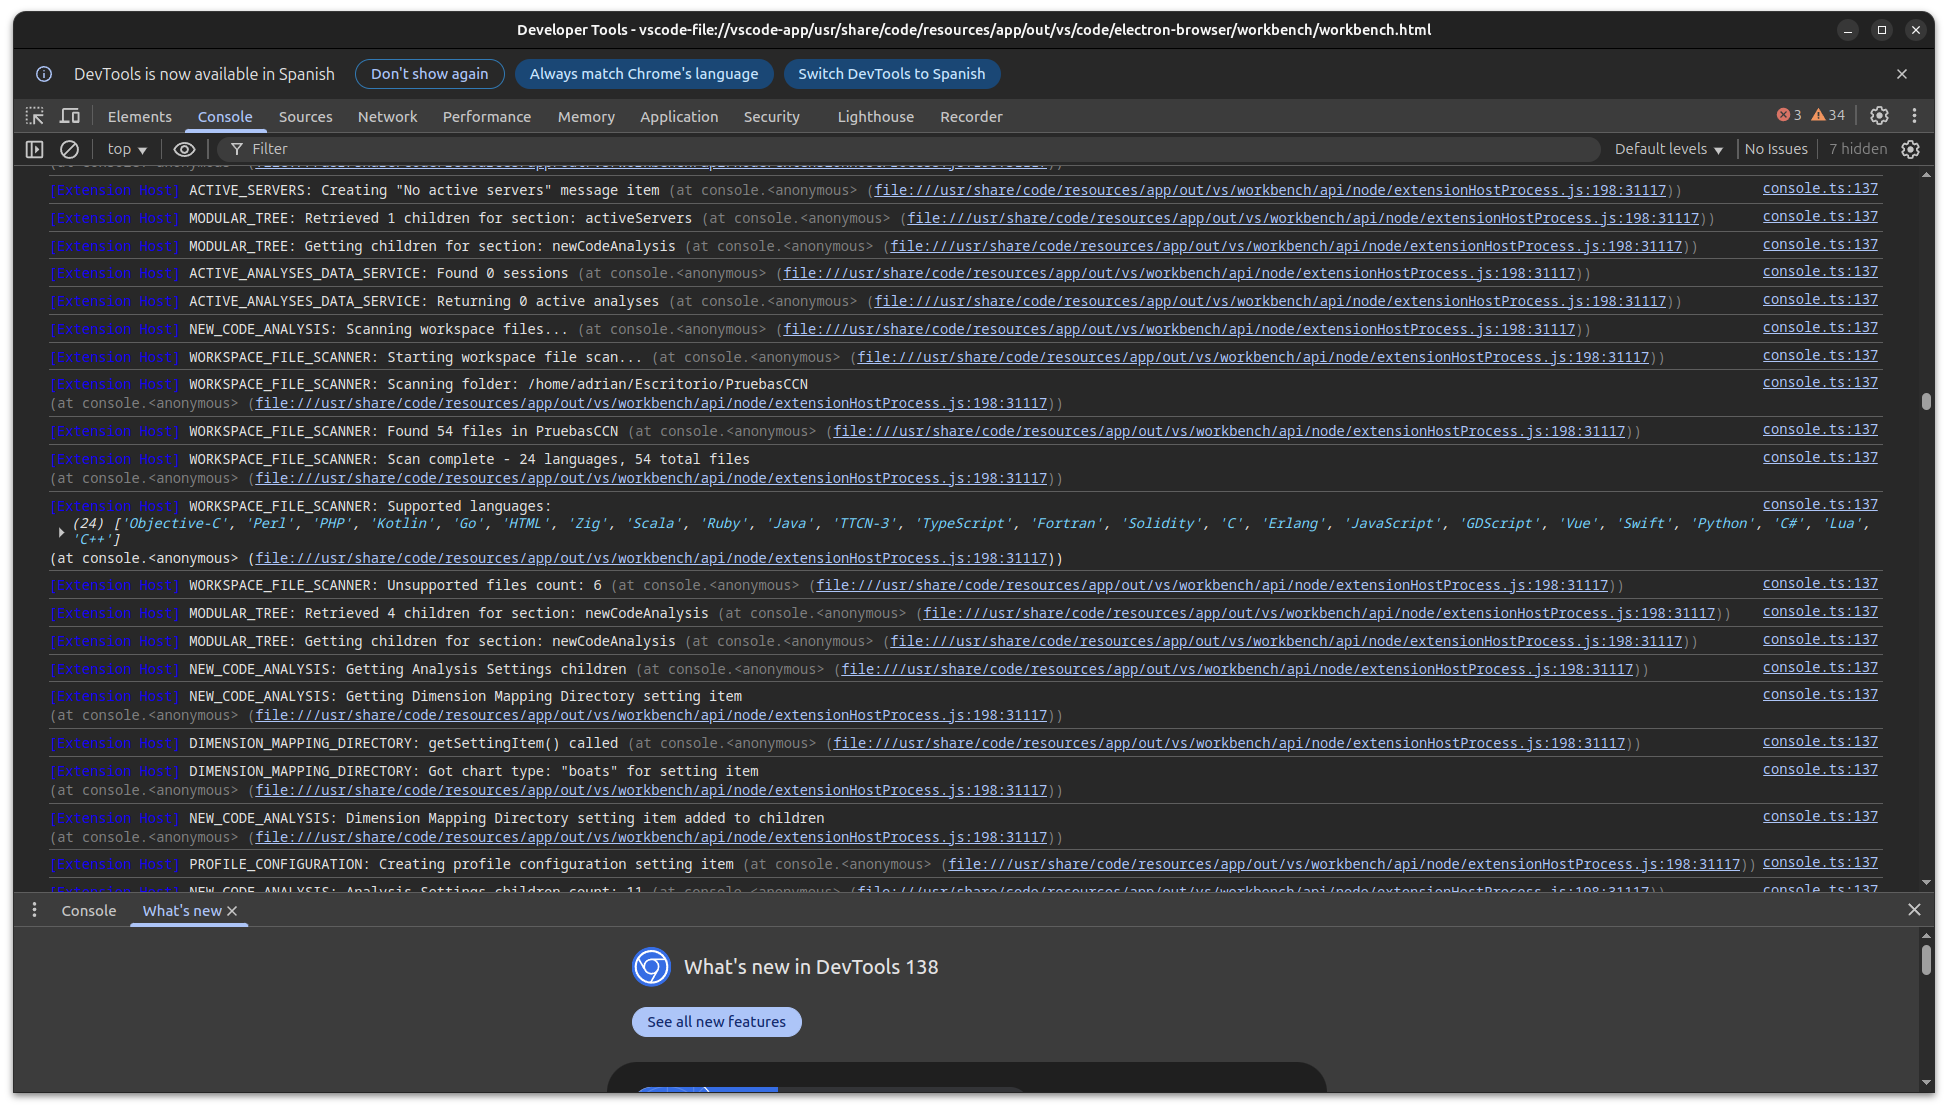
\includegraphics[width=0.9\textwidth]{img/developer-tools-logs.png}
\caption{Developer Tools de VS Code mostrando los console.logs del plugin durante la ejecución.}
\label{fig:developer-tools-logs}
\end{figure}

\section{Validación de la comunicación en tiempo real}
\label{sec:validacion-tiempo-real}

Para comprobar que la conexión SSE (Server-Sent Events) en los diferentes modos de análisis estaba funcionando correctamente, se utilizaron:

\begin{itemize}
  \item La consola de Developer Tools de VS Code
  \item La consola del navegador donde estaba abierto el análisis (de cualquier tipo)
\end{itemize}

Estas herramientas permitieron verificar que los cambios y el envío de datos mediante SSE se realizaban correctamente, confirmando que la conexión bidireccional estaba establecida y funcionando.

% TODO: Añadir imagen de la consola del navegador recibiendo actualizaciones SSE
% Nombre sugerido: img/sse-updates-browser.png

\begin{figure}[H]
\centering
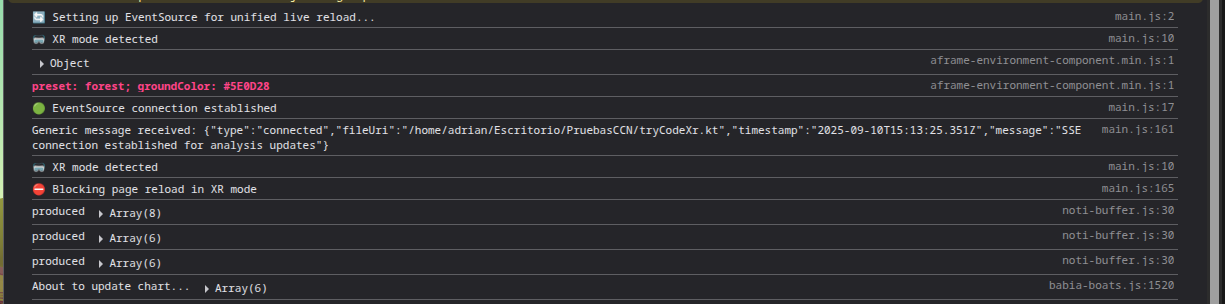
\includegraphics[width=0.9\textwidth]{img/sse-updates-browser.png}
\caption{Consola del navegador mostrando la recepción de una actualización SSE.}
\label{fig:sse-updates-browser}
\end{figure}

\section{Pruebas en entornos de realidad virtual}
\label{sec:pruebas-vr}

La comprobación del funcionamiento de las experiencias XR se realizó gracias al uso de las gafas de realidad virtual Meta Oculus Quest 3 proporcionadas por la universidad. Estas pruebas permitieron:

\begin{itemize}
  \item Probar, observar y confirmar que todo en cuanto a experiencias de realidad virtual estaba funcionando correctamente
  \item Validar la usabilidad de la interfaz en un entorno inmersivo real
  \item Verificar la correcta actualización de la visualización en tiempo real
\end{itemize}

El procedimiento para conectarse al servidor desde las gafas es sencillo: el plugin informa de la IP interna con la que se ha lanzado el servidor, y en el navegador de las gafas, estando en la misma red WiFi, se introduce esa dirección IP y puerto para disfrutar de la experiencia VR/AR.

% TODO: Añadir imagen mostrando cómo el plugin informa de la IP en la red
% Nombre sugerido: img/ip-connection-info.png

\begin{figure}[H]
\centering
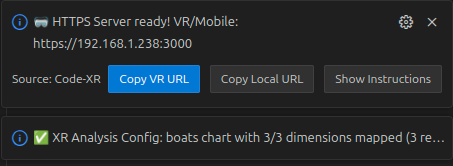
\includegraphics[width=0.9\textwidth]{img/ip-connection-info.png}
\caption{Información proporcionada por el plugin sobre la dirección IP para la conexión desde dispositivos externos.}
\label{fig:ip-connection-info}
\end{figure}


%%%%%%%%%%%%%%%%%%%%%%%%%%%%%%%%%%%%%%%%%%%%%%%%%%%%%%%%%%%%%%%%%%%%%%%%%%%%%%%%
%%%%%%%%%%%%%%%%%%%%%%%%%%%%%%%%%%%%%%%%%%%%%%%%%%%%%%%%%%%%%%%%%%%%%%%%%%%%%%%%
% RESULTADOS %
%%%%%%%%%%%%%%%%%%%%%%%%%%%%%%%%%%%%%%%%%%%%%%%%%%%%%%%%%%%%%%%%%%%%%%%%%%%%%%%%

\cleardoublepage
\chapter{Resultados}
\label{chap:resultados}

\section{Code-XR}
\label{sec:codexr-resultados}

El inicio de este TFG empezó con la intención de mostrar las métricas de análisis de ficheros únicos, es decir, solo desarrollar el análisis de fichero en formato XR. Sin embargo, el alcance del proyecto fue ampliándose progresivamente: no solo se desarrolló el modo LivePanel para análisis de ficheros, sino que también se tuvo la ambición de lograr representar el árbol DOM en experiencia XR con actualizaciones en vivo y, además, se dio el salto cualitativo de añadir análisis de directorios completos.

En todo este proceso se logró implementar las siguientes funcionalidades:

\begin{itemize}
  \item \textbf{Análisis de ficheros individuales}: Extracción de métricas como complejidad ciclomática, número de líneas y número de parámetros.
  
  \item \textbf{Visualización en modo LivePanel}: Representación bidimensional integrada en VS Code.
  
  \item \textbf{Visualización en modo XR}: Experiencia inmersiva para explorar métricas de código en entornos de realidad virtual/aumentada.
  
  \item \textbf{Visualización del árbol DOM}: Representación tridimensional de la estructura DOM de archivos HTML.
  
  \item \textbf{Análisis de directorios completos}: Procesamiento recursivo de todos los archivos en un directorio.
  
  \item \textbf{Actualizaciones en tiempo real}: Sistema de Server-Sent Events (SSE) para mantener sincronizadas las visualizaciones con cambios en el código.
  
  \item \textbf{Sistema de configuración extensible}: Opciones para personalizar el comportamiento y la apariencia de las visualizaciones.
  
  \item \textbf{Creación de escenas A-Frame/BabiaXR}: Generación dinámica de escenas XR con metáforas visuales adaptadas a diferentes tipos de datos y métricas.
  
  \item \textbf{Integración completa con la API de VS Code}: Implementación de comandos, vistas personalizadas, webviews y extensión del sistema de tareas.
  
  \item \textbf{Gestión de entornos Python}: Detección y configuración automática de entornos virtuales Python para el análisis de código sin configuración manual.
  
  \item \textbf{Sistema de servidores multiproceso}: Arquitectura que permite mantener múltiples servidores de análisis simultáneos sin bloquear la interfaz de usuario.
  
  \item \textbf{Compatibilidad multiplataforma}: Funcionamiento en Windows, macOS y Linux con adaptación automática a particularidades de cada sistema.
  
  \item \textbf{Manejo Marketplace VS Code}: Publicación y mantenimiento del plugin en el Marketplace oficial de Visual Studio Code.
  
  \item \textbf{Documentación y recursos públicos}: Creación de una página web con tutoriales, guías de instalación, ejemplos y recursos académicos.
  
\end{itemize}

El plugin además cuenta con la posibilidad de personalizar la experiencia del usuario y de disfrutar de la potencia del plugin de distintas formas adaptándose a las necesidades y preferencias específicas de cada desarrollador.

\section{Resultados en proyectos relevantes}
\label{sec:resultados-proyectos}

Para demostrar que Code-XR no es solo un concepto académico sino una herramienta con aplicación práctica real, se llevaron a cabo pruebas extensivas con tres proyectos de software reales:

\begin{table}[h]
\centering
\begin{tabular}{|l|c|l|}
\hline
\textbf{Proyecto} & \textbf{Archivos} & \textbf{Descripción} \\
\hline
BabiaXR \cite{moreno2022babiaxr} & 77 & Framework para visualización de datos en XR \\
\hline
Express.js \cite{expressjs2022web} & 142 & Framework web minimalista para Node.js \\
\hline
JetUML \cite{jetuml2022web} & 338 & Herramienta ligera para diagramas UML \\
\hline
\end{tabular}
\caption{Proyectos utilizados para validar Code-XR}
\label{tab:proyectos-validacion}
\end{table}

En todos estos proyectos se realizaron pruebas progresivas, desde el análisis de archivos individuales hasta el análisis completo de todos los archivos del proyecto, generando visualizaciones como la siguiente:

% TODO: Añadir foto de análisis de un proyecto completo
% Nombre sugerido: img/analisis-proyecto-completo.png

\begin{figure}[H]
\centering
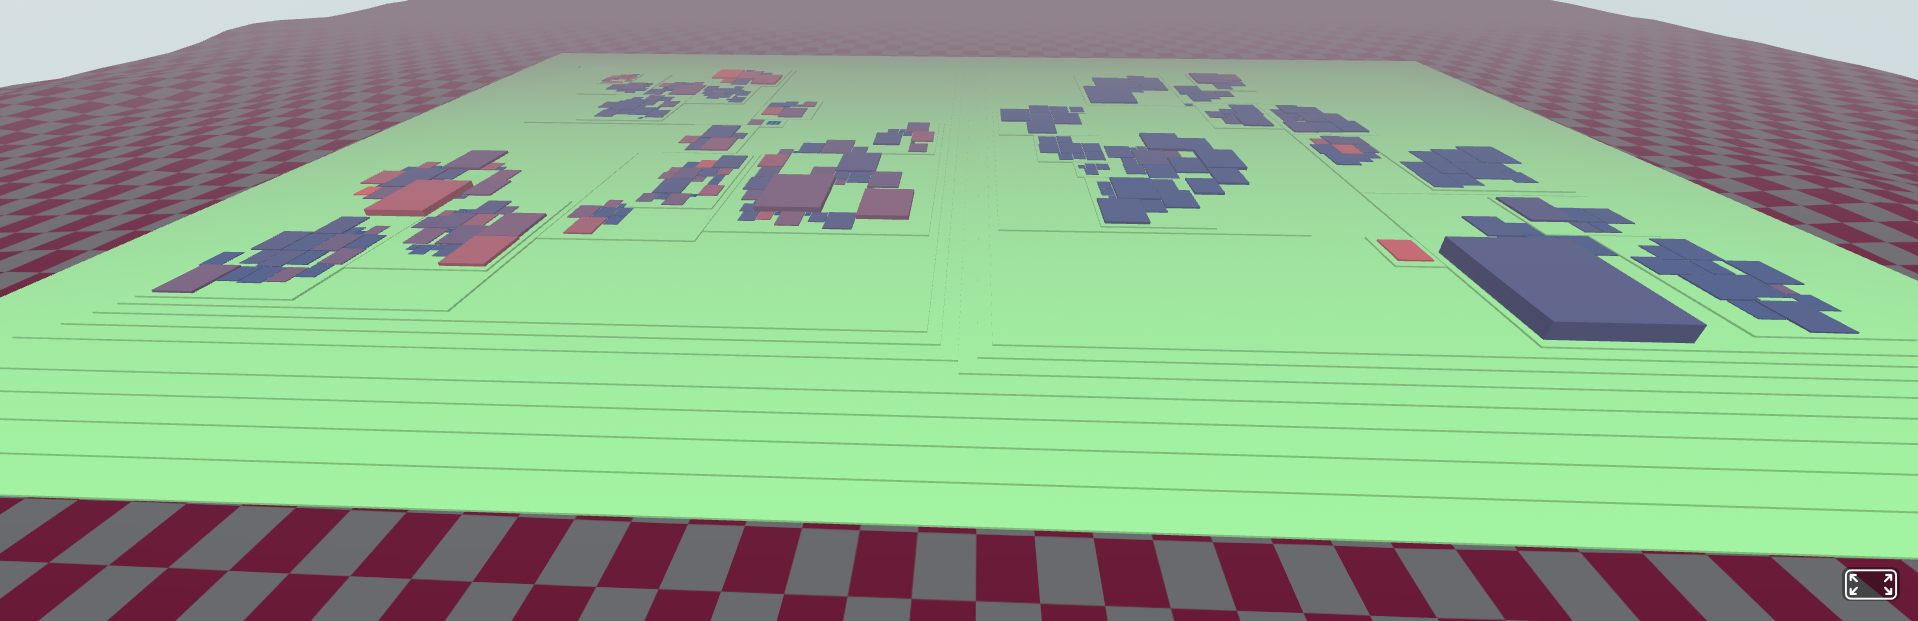
\includegraphics[width=0.9\textwidth]{img/analisis-proyecto-completo.png}
\caption{Visualización 3D de un análisis completo de proyecto con Code-XR}
\label{fig:analisis-proyecto-completo}
\end{figure}

\section{Disponibilidad del software}
\label{sec:disponibilidad-software}

Code-XR cuenta con una página web pública alojada en GitHub Pages (\url{https://amontesl.github.io/code-xr-docs/}), que sirve como punto central de acceso a toda la información relacionada con el proyecto. En esta página web se pueden encontrar:

\begin{itemize}
  \item \textbf{Galería de videos}: Colección de tutoriales y demostraciones que muestran el funcionamiento del plugin en diferentes escenarios.
  
  \item \textbf{Proyectos reales}: Sección dedicada a los tres proyectos mencionados anteriormente (BabiaXR, Express.js y JetUML) con videos específicos de cada uno y un dashboard interactivo para cada proyecto que permite previsualizar cómo se ve el análisis en XR, similar a la visualización mostrada en la Figura~\ref{fig:analisis-proyecto-completo}.
  
  \item \textbf{Guías de instalación}: Instrucciones detalladas para instalar Code-XR desde el Marketplace oficial de VS Code, mediante línea de comandos, o descargando directamente el archivo VSIX desde GitHub Releases.
  
  \item \textbf{Guía rápida de inicio}: Tutorial paso a paso para poner en marcha y realizar un primer análisis en menos de 10 minutos.
  
  \item \textbf{Recursos académicos}: En esta sección se pueden encontrar y descargar tanto este mismo documento PDF como la presentación del TFG y otros materiales relacionados con el proyecto.
\end{itemize}

\paragraph{Videos recomendados para visualizar}
Todos estos videos están disponibles en la galería de la página web. Se recomienda encarecidamente visualizarlos para contemplar todas las posibilidades de este plugin, ya que por motivos de espacio en esta memoria es imposible documentar con imágenes todos los escenarios posibles. Además, al visualizar los videos se puede llegar a ver y entender mejor el funcionamiento en tiempo real de Code-XR:

\begin{enumerate}
  \item \textbf{Interface UI}: \url{https://youtu.be/KRgLdLZJXHA}
  \item \textbf{File Analysis LivePanel Mode}: \url{https://youtu.be/n5ZcjlR4pPc}
  \item \textbf{File Analysis XR Mode}: \url{https://youtu.be/38jGwFGORvc}
  \item \textbf{Directory Analysis LivePanel Mode}: \url{https://youtu.be/sPWjcgV-gZQ}
  \item \textbf{Directory Analysis XR Mode}: \url{https://youtu.be/TnfS2SevtWU}
  \item \textbf{Análisis de un proyecto real (BabiaXR)}: \url{https://youtu.be/NluAHe3BQu8}
  \item \textbf{HTML DOM Tree Visualization}: \url{https://youtu.be/110b-AergdU}
  \item \textbf{Experiencia programar con Code-XR en AR}: \url{https://youtu.be/d7fojpP90Dk}
\end{enumerate}

El software es libre y de código abierto, disponible bajo licencia MIT en el repositorio oficial: \url{https://github.com/aMonteSl/CodeXR}\cite{code-xr}.

\section{VISSOFT/ICSME 2025}
\label{sec:vissoft-icsme}

El proyecto Code-XR fue aceptado y presentado el 7 de septiembre de 2025 en la conferencia internacional VISSOFT/ICSME 2025  (IEEE Working Conference on Software Visualization / International Conference on Software Maintenance and Evolution) \cite{vissoft2025} en la categoría de poster track.

La versión presentada (0.0.8) era ligeramente anterior a la versión actual (1.0.0) y contenía las funcionalidades de análisis de ficheros individuales y visualización del DOM, pero aún no incluía el análisis de directorios completos que se ha incorporado posteriormente.

El paper completo aceptado en la conferencia está disponible para su descarga desde la página web oficial de Code-XR en la sección de Recursos, o directamente a través del DOI permanente: \url{https://zenodo.org/records/16352142}.

\paragraph{Poster presentado en la conferencia}
El poster académico presentado durante la conferencia sintetiza visualmente las principales características y contribuciones de Code-XR, mostrando su arquitectura, funcionalidades clave y ejemplos de visualización en tiempo real. A continuación se presenta el poster completo tal como fue exhibido en el evento:

% TODO: Añadir imagen del poster presentado en VISSOFT/ICSME 2025
% Nombre sugerido: img/poster-vissoft-icsme-2025.png
\begin{figure}[H]
\centering
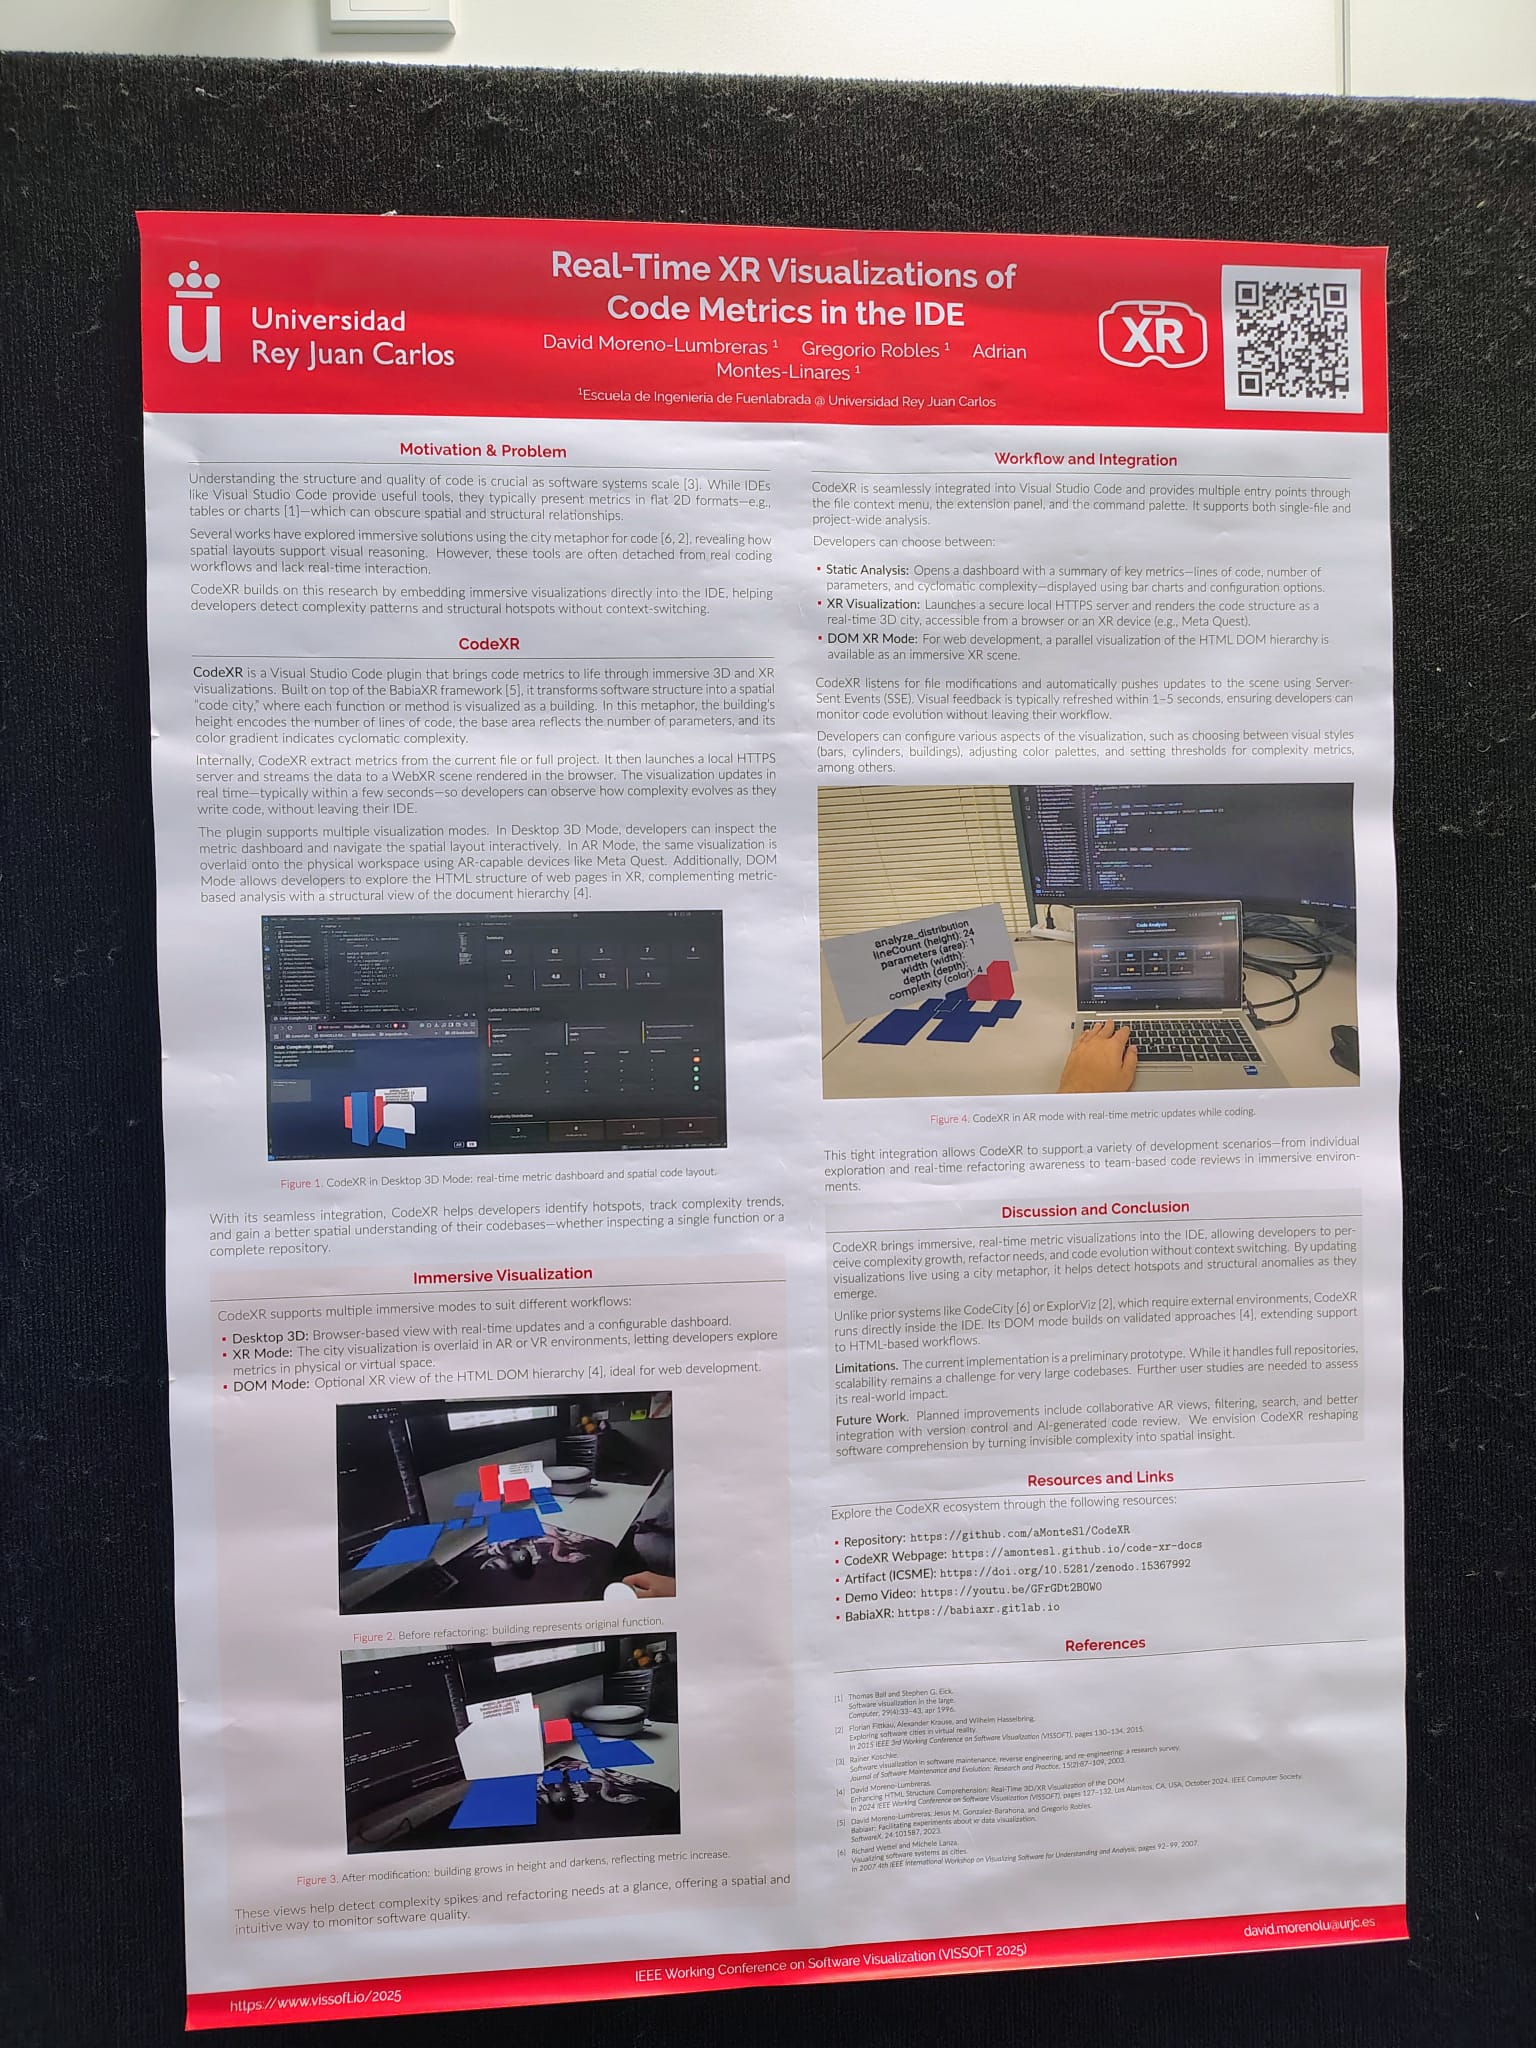
\includegraphics[width=0.45\textwidth]{img/poster-vissoft-icsme-2025.png}
\caption{Poster de Code-XR presentado en la conferencia internacional VISSOFT/ICSME 2025, mostrando la arquitectura del sistema, las principales funcionalidades y ejemplos de visualización en tiempo real.}
\label{fig:poster-vissoft-icsme}
\end{figure}

Esta aceptación en un foro académico internacional de prestigio confirma la relevancia y el valor de Code-XR como contribución al campo de la visualización de software, validando tanto su enfoque innovador como su implementación práctica.

\section{Difusión y adopción de Code-XR}
\label{sec:adopcion}

Además de su validación técnica, Code-XR ha sido publicado en el \textit{Visual Studio Code Marketplace}, lo que ha permitido evaluar de manera preliminar su grado de difusión y adopción entre la comunidad de desarrolladores. La Figura~\ref{fig:marketplace-stats} muestra las estadísticas de uso registradas en los últimos 90 días, que constituyen el rango máximo disponible en la plataforma oficial.

Durante este periodo se han alcanzado \textbf{143 nuevas adquisiciones (90 últimos días)}, acumulando un total de \textbf{271 instalaciones desde su publicación}. El gráfico de tendencias refleja una evolución sostenida con picos de actividad asociados a momentos de mayor visibilidad del proyecto (principalmente publicaciones de nuevas versiones). Cabe destacar que la tasa de conversión entre visualizaciones de la página de extensión y descargas es positiva, lo que evidencia interés real por parte de los usuarios que consultan el plugin.

Estos resultados, aunque preliminares, ponen de manifiesto que Code-XR no sólo constituye una contribución académica, sino también una herramienta con proyección práctica y potencial de crecimiento dentro de la comunidad de Visual Studio Code.

\begin{figure}[H]
\centering
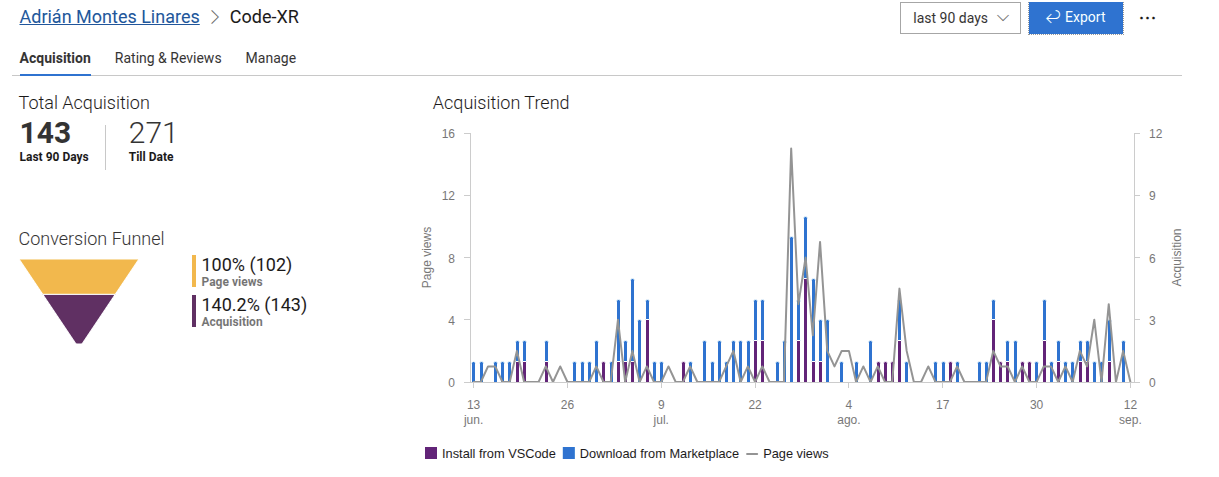
\includegraphics[width=0.95\textwidth]{img/marketplace-stats.png}
\caption{Estadísticas de adquisición de Code-XR en el \textit{Visual Studio Code Marketplace} (últimos 90 días).}
\label{fig:marketplace-stats}
\end{figure}

%%%%%%%%%%%%%%%%%%%%%%%%%%%%%%%%%%%%%%%%%%%%%%%%%%%%%%%%%%%%%%%%%%%%%%%%%%%%%%%%
%%%%%%%%%%%%%%%%%%%%%%%%%%%%%%%%%%%%%%%%%%%%%%%%%%%%%%%%%%%%%%%%%%%%%%%%%%%%%%%%
% CONCLUSIONES %
%%%%%%%%%%%%%%%%%%%%%%%%%%%%%%%%%%%%%%%%%%%%%%%%%%%%%%%%%%%%%%%%%%%%%%%%%%%%%%%%

\cleardoublepage
\chapter{Conclusiones}
\label{chap:conclusiones}


\section{Consecución de objetivos}
\label{sec:consecucion-objetivos}

Al finalizar este Trabajo Fin de Grado, se ha cumplido satisfactoriamente el objetivo principal y las contribuciones específicas planteadas para Code-XR:

\begin{itemize}
  \item \textbf{Visualización inmersiva en tiempo real}: Sistema completo implementado que permite visualizar métricas de código en tiempo real desde VS Code, capturando y procesando cambios automáticamente sin intervención manual.
  
  \item \textbf{Tecnologías web XR accesibles}: Integración exitosa de A-Frame y BabiaXR para experiencias XR accesibles desde cualquier navegador, democratizando el acceso a visualizaciones tridimensionales sin software adicional.
  
  \item \textbf{Múltiples modos de visualización}: Desarrollo completo de tres modos (LivePanel, XR Mode, DOM Mode) optimizados para diferentes casos de uso, desde análisis integrados hasta experiencias inmersivas.
  
  \item \textbf{Arquitectura extensible}: Construcción de arquitectura modular eficiente con sistema de plugins, adaptadores y múltiples opciones de configuración personalizable.
  
  \item \textbf{Análisis de directorios completos}: Capacidad implementada para análisis recursivo de proyectos completos, visualizando estructuras de software a gran escala.
  
  \item \textbf{Sistema multiproceso}: Arquitectura que mantiene múltiples servidores simultáneos, facilitando comparaciones entre diferentes componentes del código.
  
  \item \textbf{Gestión automática Python}: Detección y configuración automática de entornos virtuales, eliminando configuración manual para análisis.
\end{itemize}

Los desafíos técnicos en tiempo real y optimización se resolvieron mediante análisis incremental, procesamiento por lotes y mecanismos de debounce. La aceptación en VISSOFT/ICSME 2025 valida la relevancia científica de Code-XR como contribución al campo de visualización de software mediante tecnologías XR.

\section{Aplicación de lo aprendido}
\label{sec:aplicacion}

La realización de este TFG ha permitido aplicar y consolidar conocimientos adquiridos durante el Grado, integrando múltiples asignaturas en el desarrollo de Code-XR:

\begin{enumerate}
  \item \textbf{Sistemas Telemáticos}: Conocimientos sobre estructura DOM y modelo cliente-servidor cruciales para desarrollar DOM Mode. El modelo Modelo-Vista-Controlador facilitó la arquitectura correcta, especialmente la separación entre motor de análisis y visualizaciones.
  
  \item \textbf{Aplicaciones Telemáticas}: Profundización en HTML y JavaScript imprescindible para implementar visualizaciones A-Frame/BabiaXR, desarrollando estructura visual tridimensional y lógica de interacción XR.
  
  \item \textbf{Robótica}: Introducción a Git, fundamental durante el desarrollo para mantener historial ordenado, facilitar experimentación y gestionar versiones publicadas eficientemente.
  
  \item \textbf{Seguridad en Redes}: Conceptos de nonce y hash aplicados especialmente en el sistema de detección de cambios mediante hash de contenido.
  
  \item \textbf{Sistemas Distribuidos}: Conocimientos básicos para manejar múltiples análisis paralelos, fundamental para la implementación multiproceso y coordinación entre componentes.
  
  \item \textbf{Sistemas Operativos}: Dominio de terminal Linux esencial para gestión del entorno de trabajo, configuración de servicios y ejecución eficiente de procesos de soporte.
\end{enumerate}

La integración de estos conocimientos fue esencial para superar retos técnicos como comunicación en tiempo real IDE-visualizaciones, gestión eficiente de recursos y procesos, y creación de experiencias interactivas tridimensionales. Este TFG sirvió como culminación práctica de la formación recibida, demostrando la capacidad de aplicar conocimientos teóricos a un proyecto real con impacto tangible.


\section{Lecciones aprendidas}
\label{sec:lecciones_aprendidas}

El desarrollo de Code-XR ha proporcionado aprendizajes técnicos y metodológicos valiosos:

\begin{enumerate}
\item \textbf{Integración de tecnologías heterogéneas}: La combinación de entornos diversos (VS Code API, Node.js, Python, A-Frame, BabiaXR) converge en soluciones innovadoras estableciendo interfaces de comunicación claras entre componentes.
  
  \item \textbf{Diseño arquitectónico inicial}: El diseño modular facilitó ampliaciones posteriores. La separación entre análisis, visualización y comunicación permitió añadir funcionalidades (análisis de directorios) sin reescribir código existente.
  
  \item \textbf{Retroalimentación temprana}: El desarrollo incremental con versiones funcionales desde etapas iniciales resultó fundamental para detectar problemas de rendimiento y usabilidad tempranamente. El enfoque "mostrar en lugar de explicar" facilitó la validación continua.
  
  \item \textbf{Optimización continua}: Las estrategias de optimización (análisis incremental, caché, procesamiento por lotes) deben incorporarse iterativamente identificando cuellos de botella. El sistema de watchers y debounce fue refinado repetidamente buscando equilibrio entre reactividad y eficiencia.
  
  \item \textbf{Documentación integral}: Mantener documentación actualizada resultó tan importante como el código, especialmente para plantillas y API de eventos. La documentación clara facilitó implementación de nuevas características y creación de materiales académicos.
  
  \item \textbf{Tecnologías web para XR}: El uso de tecnologías web estándar (A-Frame/WebXR) versus plataformas propietarias permitió experiencias XR accesibles desde cualquier navegador, confirmando la democratización de visualizaciones inmersivas sin hardware especializado.
  
  \item \textbf{Gestión de versiones}: El proceso Marketplace VS Code enseñó importancia del versionado semántico. Las múltiples versiones (0.0.1 a 1.0.0) permitieron iteración rápida y retroalimentación de usuarios reales.
  
  \item \textbf{Experiencia de usuario (UX)}: Desarrollar interfaces intuitivas resultó tan crítico como la funcionalidad técnica. Los usuarios valoran simplicidad y resultados inmediatos sin configuración compleja.
  
  \item \textbf{Comunicación y promoción (soft skills)}: La creación de contenido multimedia, documentación atractiva y presentación en VISSOFT/ICSME 2025 fueron habilidades esenciales. Comunicar ventajas técnicas accesiblemente para diferentes audiencias resultó fundamental para adopción.
  
  \item \textbf{Gestión del alcance}: Equilibrar ambición técnica con viabilidad práctica. La evolución gradual desde objetivos modestos (análisis individual) hacia funcionalidades complejas (análisis directorios, múltiples modos) mantuvo calidad evitando complejidad excesiva.
  
  \item \textbf{Validación real}: Las pruebas con proyectos reales (BabiaXR, Express.js, JetUML) identificaron limitaciones y casos no contemplados. Los prototipos académicos deben someterse a pruebas con datos reales para verificar utilidad y robustez.
\end{enumerate}

Estas lecciones contribuyeron al éxito del proyecto y constituyen conocimientos aplicables a futuros desarrollos en visualización de software y tecnologías XR. Las habilidades blandas desarrolladas durante promoción y difusión demostraron ser tan valiosas como las competencias técnicas para el éxito integral.


\section{Trabajos futuros}
\label{sec:trabajos_futuros}

Code-XR presenta numerosas direcciones de expansión futuras como base para otros TFGs o desarrollos avanzados:

\begin{enumerate}
  \item \textbf{Ampliación de métricas disponibles}: Incorporar métricas avanzadas como deuda técnica, cobertura de pruebas, acoplamiento entre componentes y cohesión de módulos para análisis más sofisticados sobre calidad y mantenibilidad del código.
  
  \item \textbf{Experiencias colaborativas multipersona}: Sistema multiusuario para visualizar y trabajar simultáneamente sobre análisis, facilitando sesiones de revisión en equipo con avatares representativos y herramientas para destacar y discutir aspectos específicos en tiempo real.

  \item \textbf{Proyección de interfaz VS Code en XR}: Captura y retransmisión de la ventana del editor dentro del entorno XR, permitiendo consultar y modificar código sin depender de monitores físicos, mejorando la integración fluida entre programación y visualización.

  \item \textbf{Integración con control de versiones}: Visualización temporal de la evolución del código mostrando cambios de métricas y estructura entre commits, proporcionando perspectiva histórica sobre calidad del software e identificación de problemas potenciales.
  
  \item \textbf{Análisis predictivo mediante IA}: Modelos de aprendizaje automático para predecir áreas propensas a errores o refactorización, entrenados con datos históricos para identificar patrones que precedan la introducción de defectos.
    
  \item \textbf{Interfaces gestuales avanzadas}: Controles gestuales sofisticados para manipular, filtrar y analizar código mediante gestos naturales, mejorando significativamente la experiencia en dispositivos VR como Meta Quest.
  \end{enumerate}

Estas propuestas ampliarían las capacidades de Code-XR abriendo nuevas posibilidades de investigación en visualización de software, experiencias inmersivas y herramientas de desarrollo colaborativo.


%%%%%%%%%%%%%%%%%%%%%%%%%%%%%%%%%%%%%%%%%%%%%%%%%%%%%%%%%%%%%%%%%%%%%%%%%%%%%%%%
%%%%%%%%%%%%%%%%%%%%%%%%%%%%%%%%%%%%%%%%%%%%%%%%%%%%%%%%%%%%%%%%%%%%%%%%%%%%%%%%
% APÉNDICE(S) %
%%%%%%%%%%%%%%%%%%%%%%%%%%%%%%%%%%%%%%%%%%%%%%%%%%%%%%%%%%%%%%%%%%%%%%%%%%%%%%%%

\cleardoublepage
\appendix
\chapter{Manual de usuario}
\label{app:manual}

El plugin es bastante sencillo de entender en cuanto a su manejo gracias a la interfaz gráfica. De todas formas, se dispone de un video tutorial en la página web oficial del plugin, el cual detalla qué hace cada sección.

Para aquellos que quieran ver directamente el tutorial, pueden acceder a través del siguiente enlace: \url{https://youtu.be/KRgLdLZJXHA}

%%%%%%%%%%%%%%%%%%%%%%%%%%%%%%%%%%%%%%%%%%%%%%%%%%%%%%%%%%%%%%%%%%%%%%%%%%%%%%%%
%%%%%%%%%%%%%%%%%%%%%%%%%%%%%%%%%%%%%%%%%%%%%%%%%%%%%%%%%%%%%%%%%%%%%%%%%%%%%%%%
% BIBLIOGRAFIA %
%%%%%%%%%%%%%%%%%%%%%%%%%%%%%%%%%%%%%%%%%%%%%%%%%%%%%%%%%%%%%%%%%%%%%%%%%%%%%%%%

\cleardoublepage

% Las siguientes dos instrucciones es todo lo que necesitas
% para incluir las citas en la memoria
\bibliographystyle{abbrv}
\bibliography{memoria}  % memoria.bib es el nombre del fichero que contiene
% las referencias bibliográficas. Abre ese fichero y mira el formato que tiene,
% que se conoce como BibTeX. Hay muchos sitios que exportan referencias en
% formato BibTeX. Prueba a buscar en http://scholar.google.com por referencias
% y verás que lo puedes hacer de manera sencilla.
% Más información: 
% http://texblog.org/2014/04/22/using-google-scholar-to-download-bibtex-citations/

\end{document}
